\documentclass{article}
\usepackage[utf8]{inputenc}
\usepackage{mathtools}
\usepackage{gensymb}
\usepackage{amstext}
\usepackage{amsmath}
\usepackage{graphicx}
\usepackage{textcomp}
\usepackage{float}
\usepackage{varioref}
\usepackage{fancyref}
\usepackage{caption}
\usepackage{subcaption}
\usepackage{comment}
\usepackage{hyperref}
\hypersetup{
    colorlinks=true,       % false: boxed links; true: colored links
    linkcolor=red,          % color of internal links (change box color with linkbordercolor)
    citecolor=green,        % color of links to bibliography
    filecolor=magenta,      % color of file links
    urlcolor=blue           % color of external links
}
\usepackage{epstopdf}
\usepackage[margin=1in, paperwidth=8.5in, paperheight=11in]{geometry}
\usepackage{gensymb}
\usepackage{listings}
\usepackage{xcolor}
\usepackage{listings}
\usepackage{pdfpages}
\usepackage{graphicx}
\usepackage{wrapfig}
\usepackage{lscape}
\usepackage{rotating}
\usepackage{epstopdf}
\usepackage{fancyhdr}
\usepackage{amssymb}
\usepackage{adjustbox}
\usepackage{lastpage}

\graphicspath{{images/}}

\title{Formula Hybrid: ESF Part 2}
\author{Lisa Hachmann}
\date{February 2016}

\begin{document}

\pagestyle{fancy}
\renewcommand{\headrulewidth}{0pt}
\lhead{}
\chead{}
\rhead{}
\lfoot{Page \thepage \hspace{1pt} of \pageref{LastPage}}
\cfoot{} % comment for default page numbering
\rfoot{
\includegraphics[width=2cm]{revo.png}}

\newpage

\begin{figure}[H]
    \centering
    
\includegraphics[width = 0.7 \textwidth]{FHlogo}
    % \label{fig:my_label}
\end{figure}

\vfill

\title{16 Formula Hybrid Electrical System Form (ESF)}

\section*{INTRODUCTION}
    The goal of the ESF is to ensure that vehicles are as safe as possible, and that they comply with the Formula-Hybrid completion rules. The ESF is divided seven main sections:

    \begin{enumerate}
        \item Overview
        \item Cables, Fusing \& Grounding \item Isolation \& Insulation
        \item Electric Tractive System
        \item Accumulator System
        \item Safety Controls and Indicators
        \item GLV System
    \end{enumerate}

    The Cables and Fusing, and Insulation and Isolation sections are at the beginning of the ESF as these are the areas where teams most often have trouble in complying with FH rules.\\

    A clear, concise ESF will help you to build a better car. It will also help you to pass tech testing as most common tech problems can be addressed before the car reaches the track.\\

        \textcolor{red}{\textbf{IMPORTANT INSTRUCTIONS AND REQUIREMENTS}}

    \begin{enumerate}
        \item Every part of this ESF must be filled with content. If a section is not relevant to your vehicle, mark it as “N/A” and describe briefly why not.
        \item Leave the written instructions in place and add your responses below them.
        \item All figures and tables must be included. An ESF with incomplete tables or figures will be rejected.
        \item The maximum length of a complete ESF is 100 pages.
        \item Note that many fields ask for information that was submitted in your ESF-1. This information must be reentered – in some cases will be different than what was entered in ESF-1, which is OK.
        \item When completed, this document must be converted to a pdf and submitted to: http://formula-hybrid.com/uploads/
    \end{enumerate}

    Please submit any questions, corrections and suggestions for improvement to: http://www.formula-hybrid.org/level2/support

    \newpage

    \textbf{REVIEW PROCESS}

        Once submitted, your ESF will be reviewed by at least two FH reviewers. One will be the designated primary reviewer for your team.\\

        Feedback on your ESF occurs through the Formula Hybrid upload system. You will receive emails via this system from your reviewers offering guidance and feedback. You will also submit revised versions of your ESF in this system. When you submit a revised ESF, please indicate the REVISION DATE AND LETTER (starting with Letter A) and which sections have been updated in the following table:

        \begin{table}[H]
            \centering
            \begin{tabular}{|l|l|}
            \hline
            REVISION DATE &  \\ \hline
            REVISION (A, B, C, etc...) &  \\ \hline
            \multicolumn{1}{|c|}{Section} & \multicolumn{1}{c|}{Revised (Yes/No)} \\ \hline
            1- Overview &  \\ \hline
            2- Cables and Fusing &  Yes \\ \hline
            3- Insulation and Isolation &  \\ \hline
            4- Electric Tractive System &  \\ \hline
            5- Accumulator System &  \\ \hline
            6- GLV System &  \\ \hline
            7- Safety Controls and Indicators &  \\ \hline
            8- Appendices/Datasheets &  \\ \hline
            \end{tabular}
        \end{table}

\begin{titlepage}
    \centering
    \vfill

    
\includegraphics[width=10cm]{revo.png}

    {\bfseries\Large
        REVO Electric Racing\\
        \vskip2cm
        ESF Part 2\\
    }
    \vfill
    \begin{figure}[H]
        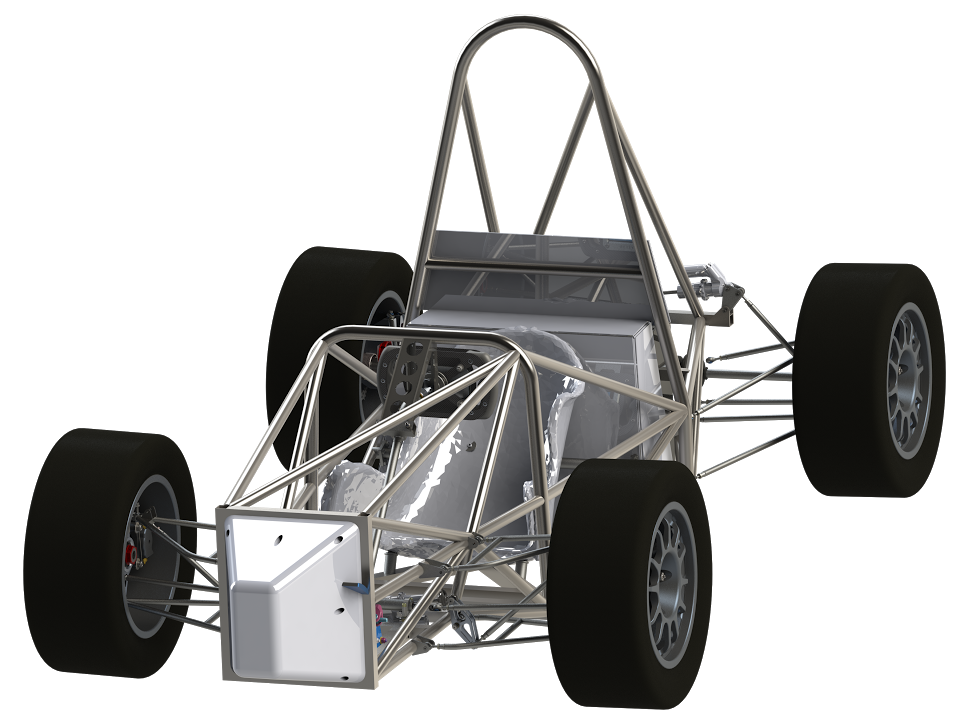
\includegraphics[width=0.4\textwidth]{carRender.png}
        \centering
    \end{figure}

    \vfill
    \begin{figure}[H]
        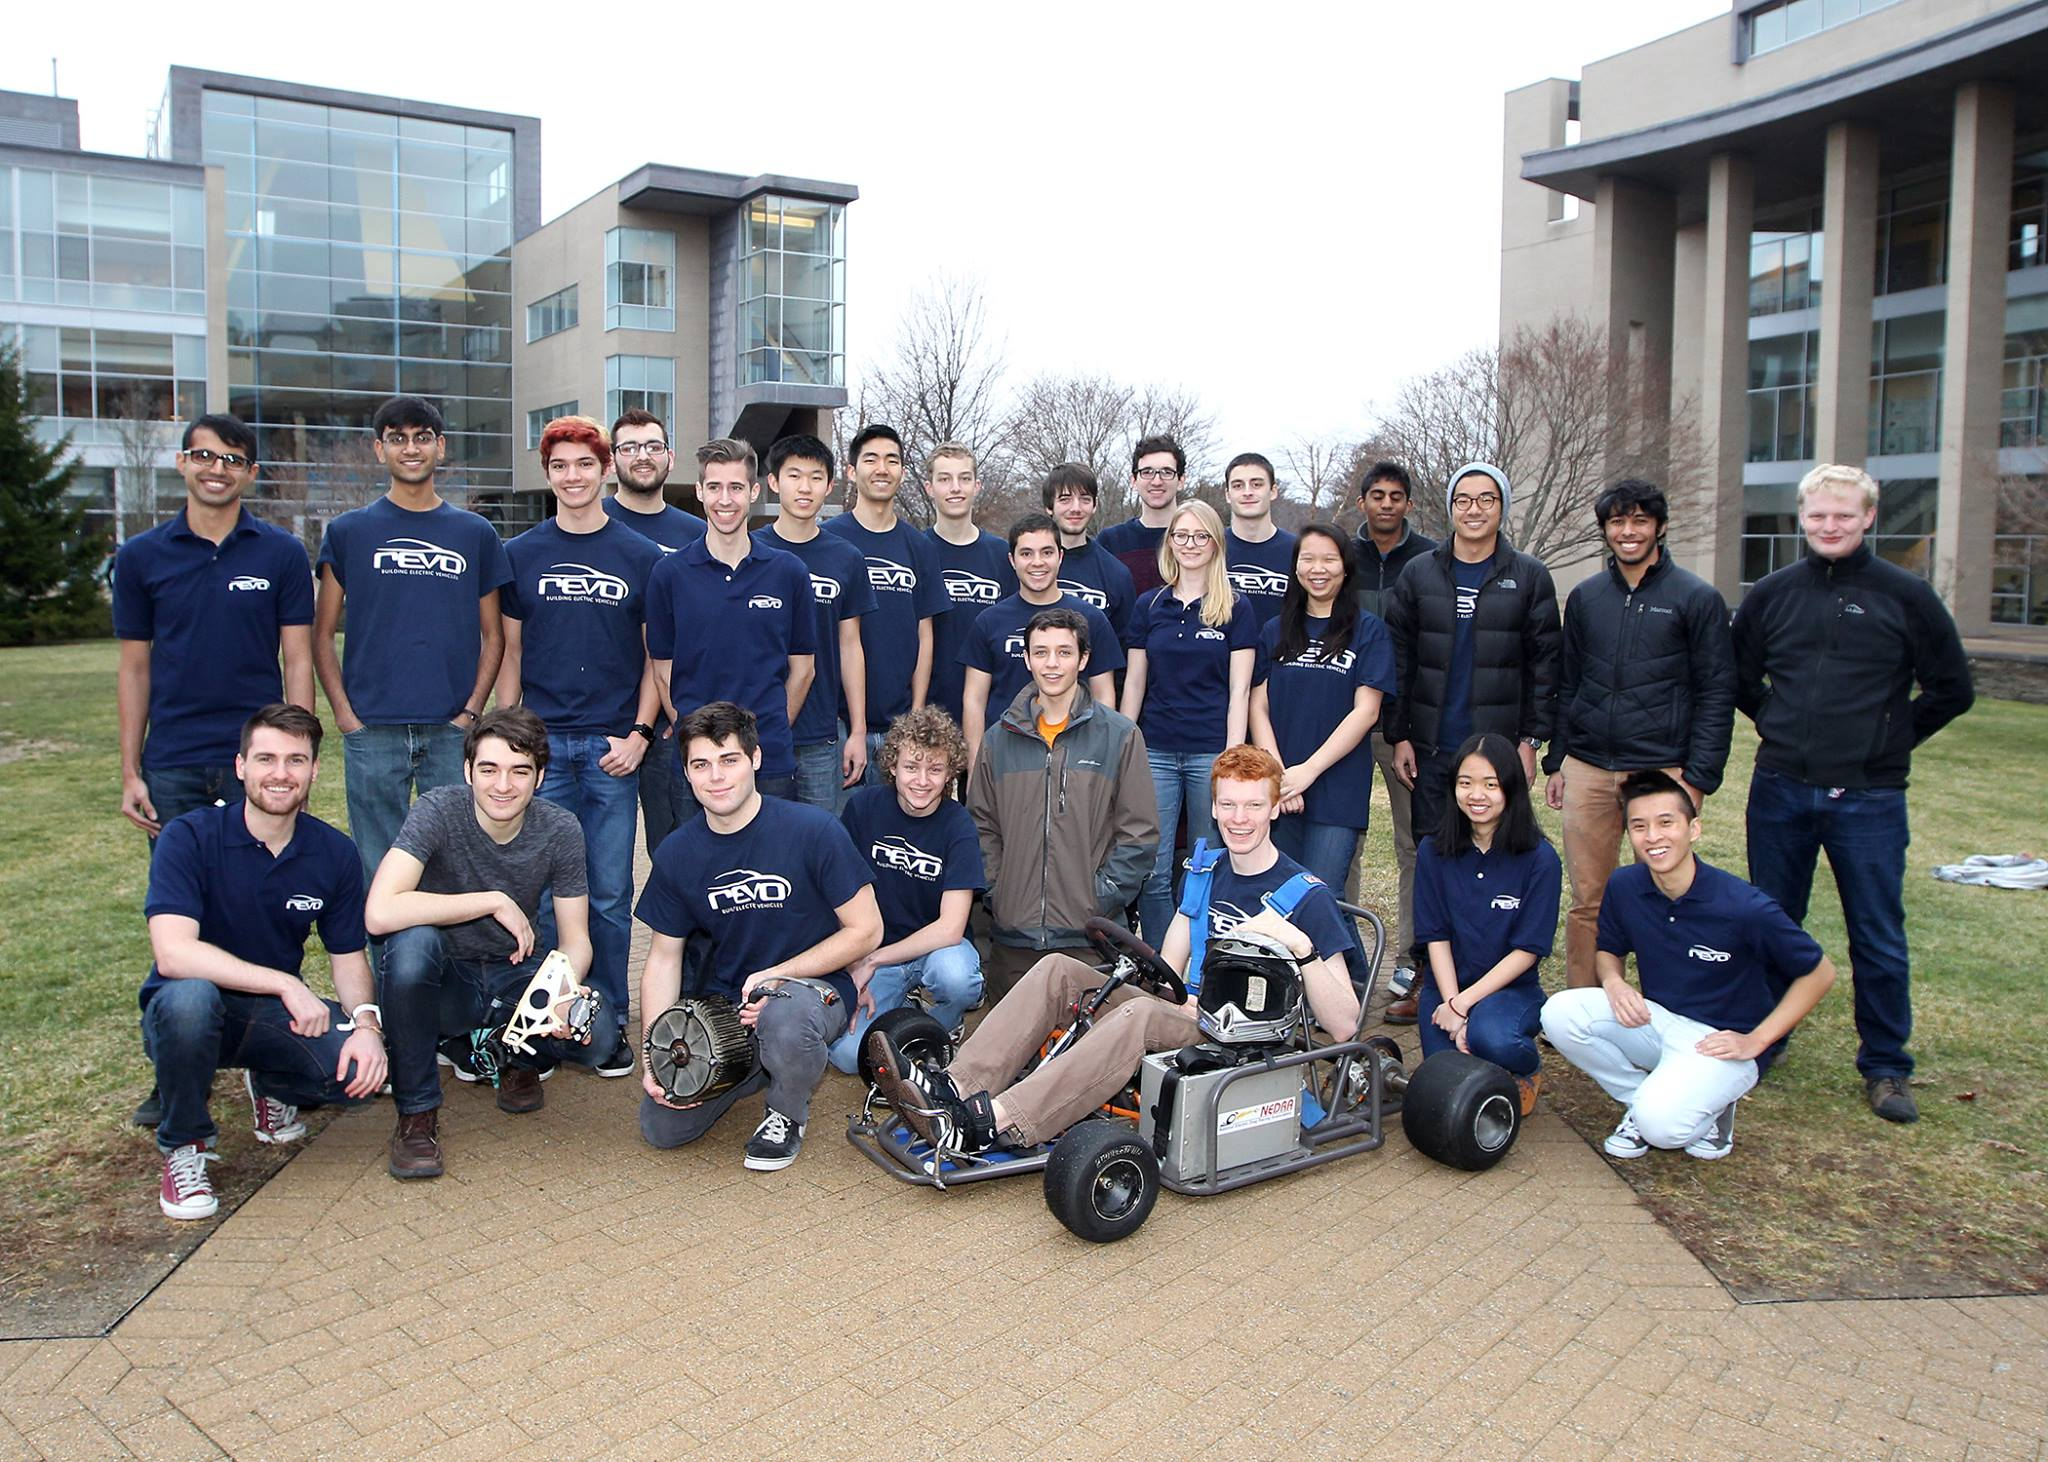
\includegraphics[width=0.4\textwidth]{teamphoto.jpg}
        \centering
    \end{figure}
    \vfill

    \begin{table}[H]
        \centering
        \label{teaminfo}
        \begin{tabular}{lr}
        University Name: & Olin College of Engineering \\ \hline
        Team Name: & REVO Electric Racing \\ \hline
        Car Number: & E212 \\ \hline
        \end{tabular}
    \end{table}

\textbf{\underline{Main Team Contact for ESF related questions:}}

    \begin{table}[H]
        \centering
        \label{overallresponsible}
        \begin{tabular}{lr}
        Name: & Lisa J. Hachmann \\ \hline
        email: & lisa.hachmann@students.olin.edu  \\ \hline
        \end{tabular}
    \end{table}
    \vfill

\end{titlepage}

\tableofcontents
\listoffigures


\setlength{\parindent}{0pt}

\newpage

\listoftables
\addcontentsline{toc}{section}{List of Tables}

\newpage

\section*{List of Abbreviations}
    \addcontentsline{toc}{section}{List of Abbreviations}
        \begin{itemize}
        \item AIR- Accumulator Isolation Relay
        \item AMS- Accumulator Management System
        \item GLV- Grounded Low-Voltage
        \item IMD- Insulation Monitoring Device
        \item SMD- Segment Maintenance Disconnect
        \item MSD- Manual Service Disconnect
        \item TS- Tractive System
        \item TSEL- Tractive System Energized Light
        \item TSMP- Tractive System Measurement Point
        \item TSV- Tractive System Voltage
        \item TSVP- Tractive System Voltage Present
        \item CONN- Main accumulator connector
        \item NDA- Non-Disclosure Agreement
        \end{itemize}

    %Add more as needed

\newpage

\section{Vehicle Overview}
    Person primarily responsible for this section:

    \begin{table}[H]
        \centering
        \label{responsible1}
        \begin{tabular}{lr}
        Name: & Lisa Hachmann \\ \hline
        e-mail: & Lisa.Hachmann@students.olin.edu \\ \hline
        \end{tabular}
    \end{table}

    Check the appropriate boxes:\\

    \par{Vehicle is:}
    \begin{itemize}
        \item \makebox[0pt][l]{$\square$}\raisebox{.15ex}{\hspace{0.1em}$\checkmark$} \hspace{0.2cm} New (built on an entirely new frame)
        \item \makebox[0pt][l]{$\square$}\raisebox{.15ex}{\hspace{0.1em}} \hspace{0.2cm} New, but built on a pre-existing frame (FSAE, FS, FH electric-only, etc.)
        \item \makebox[0pt][l]{$\square$}\raisebox{.15ex}{\hspace{0.1em}} \hspace{0.2cm} Updated from a previous year vehicle
    \end{itemize}

    \par{Architecture:}
    \begin{itemize}
        \item \makebox[0pt][l]{$\square$}\raisebox{.15ex}{\hspace{0.1em}} \hspace{0.2cm} Hybrid
        \item \makebox[0pt][l]{$\square$}\raisebox{.15ex}{\hspace{0.1em}} \hspace{0.2cm} Hybrid in Progress (HIP)
        \item \makebox[0pt][l]{$\square$}\raisebox{.15ex}{\hspace{0.1em}$\checkmark$} \hspace{0.2cm} Electric Only
    \end{itemize}

    \par{Drive:}
    \begin{itemize}
        \item \makebox[0pt][l]{$\square$}\raisebox{.15ex}{\hspace{0.1em}} \hspace{0.2cm} Front Wheel
        \item \makebox[0pt][l]{$\square$}\raisebox{.15ex}{\hspace{0.1em}$\checkmark$} \hspace{0.2cm} Rear Wheel
        \item \makebox[0pt][l]{$\square$}\raisebox{.15ex}{\hspace{0.1em}} \hspace{0.2cm} All-wheel
    \end{itemize}

    \par{Regenerative Braking:}
    \begin{itemize}
        \item \makebox[0pt][l]{$\square$}\raisebox{.15ex}{\hspace{0.1em}} \hspace{0.2cm} Front Wheels
        \item \makebox[0pt][l]{$\square$}\raisebox{.15ex}{\hspace{0.1em}$\checkmark$} \hspace{0.2cm} Rear Wheels
        \item \makebox[0pt][l]{$\square$}\raisebox{.15ex}{\hspace{0.1em}} \hspace{0.2cm} All-wheels
        \item \makebox[0pt][l]{$\square$}\raisebox{.15ex}{\hspace{0.1em}} \hspace{0.2cm} None
    \end{itemize}

\newpage

        \textit{Provide a brief, concise description of the vehicles main electrical systems including tractive system, accumulator, hybrid type (series or parallel) and method of mechanical coupling to wheels. Describe any innovative or unusual aspects of the design.}\\

        We have designed an all-electric car powered by 2 Zero Motorcycles Z-Force brushless DC motors coupled to Sevcon Gen 4 Size 4 motor controllers. The motors independently drive the rear wheels through two single speed chain reductions. Independent drive allows us to implement a virtual differential drive mode and eventually torque vectoring. The accumulator comprises 12 Nissan Leaf modules in series, which in total provides 96.4V and 65Ah of capacity. The car communicates across a CAN-Bus system, simplifying wiring substantially.\\

        \textit{Include the following figures:}

 \begin{sidewaysfigure}[p]
            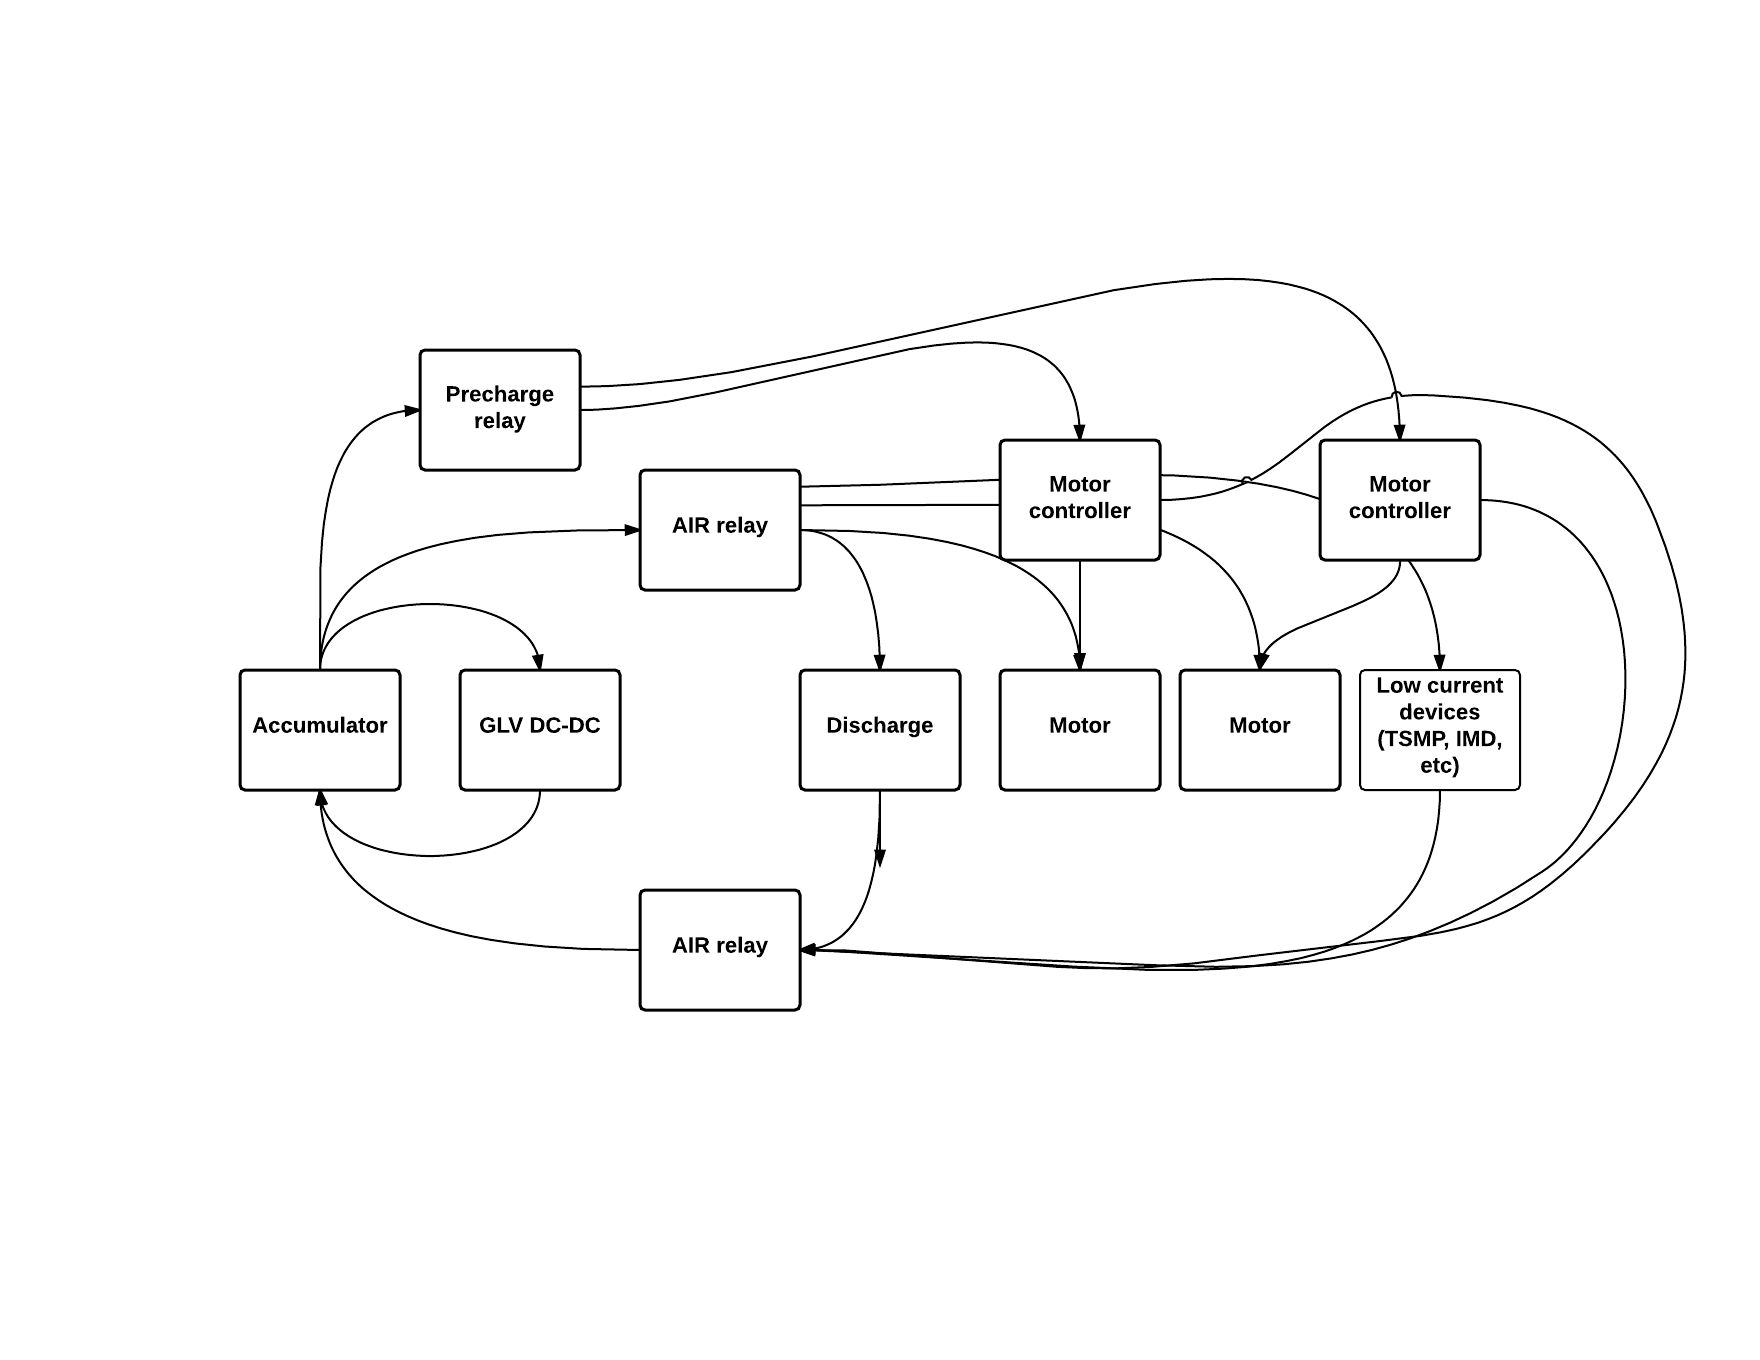
\includegraphics[width=\textheight]{TSBLOCK}
            \caption{Tractive System Block Diagram}
            \label{tractiveblock}
        \end{sidewaysfigure}

        \begin{itemize}
            \item \textit{Figure 1 – an electrical system block diagram showing all major parts associated with the tractive-system. (Not detailed wiring).}
            \item \textit{Figure 2 – Drawings or photographs showing the vehicle from the front, top, and side}
            \item \textit{Figure 3 – A wiring diagram superimposed on a top view of the vehicle showing the locations of all major TS components and the routing of TS wiring.}
            \item \textit{Figure 4 -- Include a complete TSV wiring schematic per FH Rule S4.4.1 showing connections between all TS components. This should include accumulator cells, AIRs, SMDs, motor controller, motor, pre-charge and discharge circuits, AMD, IMD, charging port and any other TS connections. \underline{\textcolor{red}{NOTE: Figure 4 is the most important diagram in the ESF}}}
        \end{itemize}

Please note that the figure numbers in our document do not correspond to the specified numbering above (Figure 2 comprises 3 figures: top, front, side view of the vehicle).

 \newpage


\newpage
\newpage
        \begin{figure}[H]
            \centering
            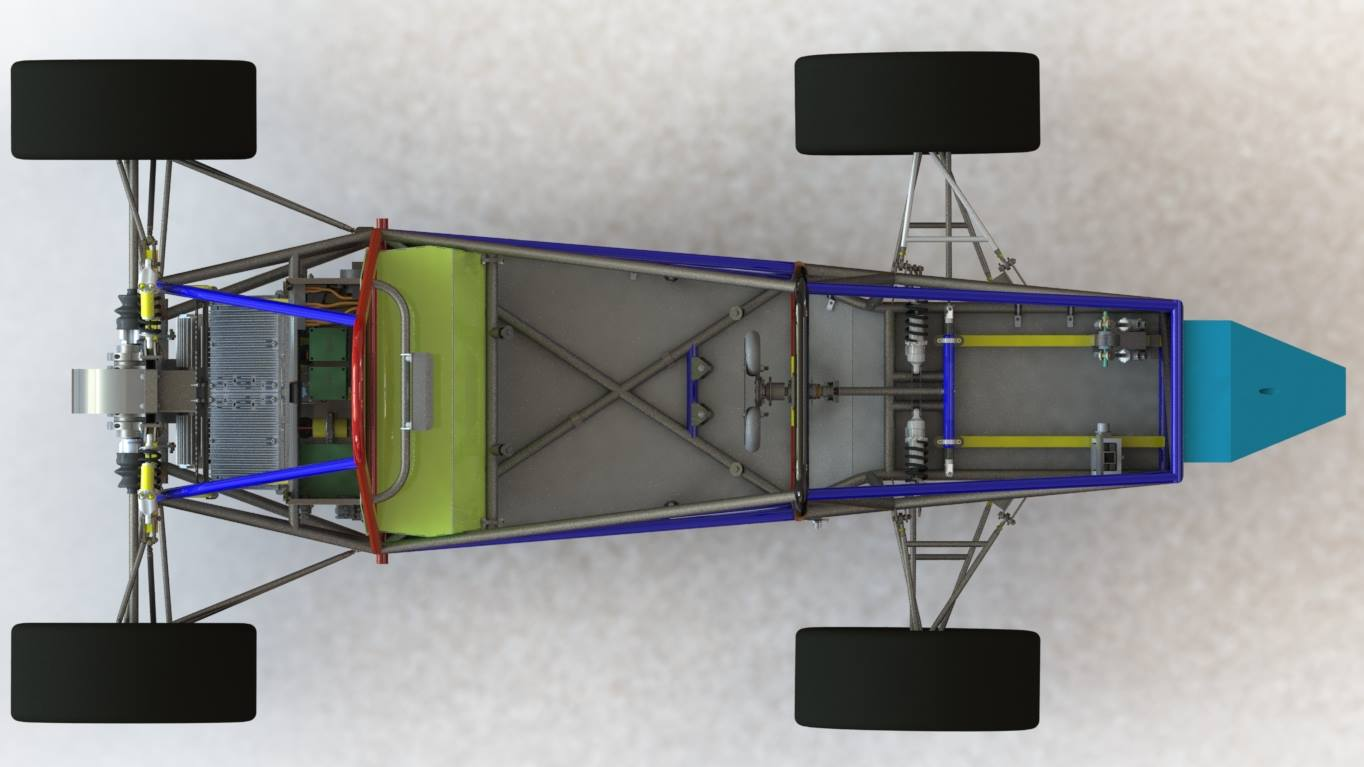
\includegraphics[width = 0.7 \textwidth]{cartopdown}
            \caption{Full Vehicle, Top View}
            \label{cartopdown}
        \end{figure}

        \begin{figure}[H]
            \centering
            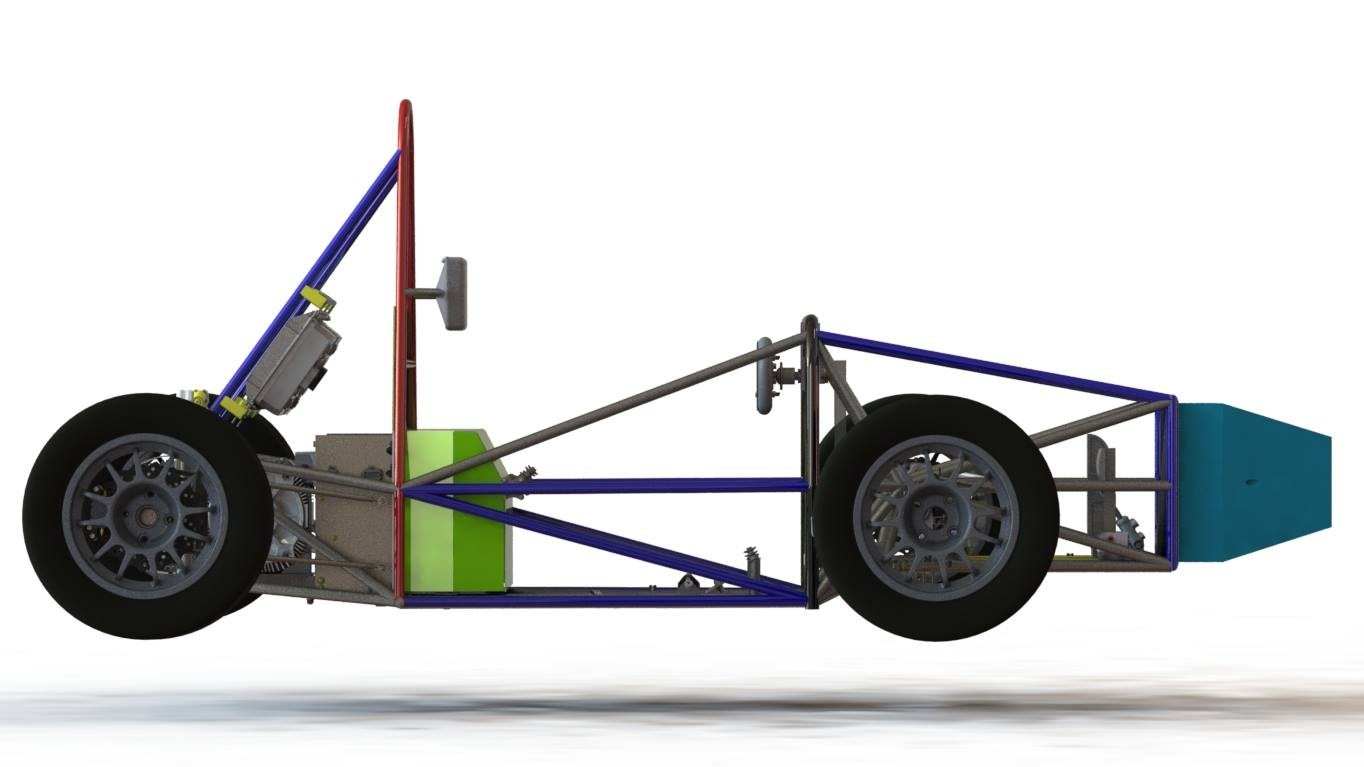
\includegraphics[width = 0.7 \textwidth]{carsideview}
            \caption{Full Vehicle, Side View}
            \label{carsideview}
        \end{figure}

        \begin{figure}[H]
            \centering
            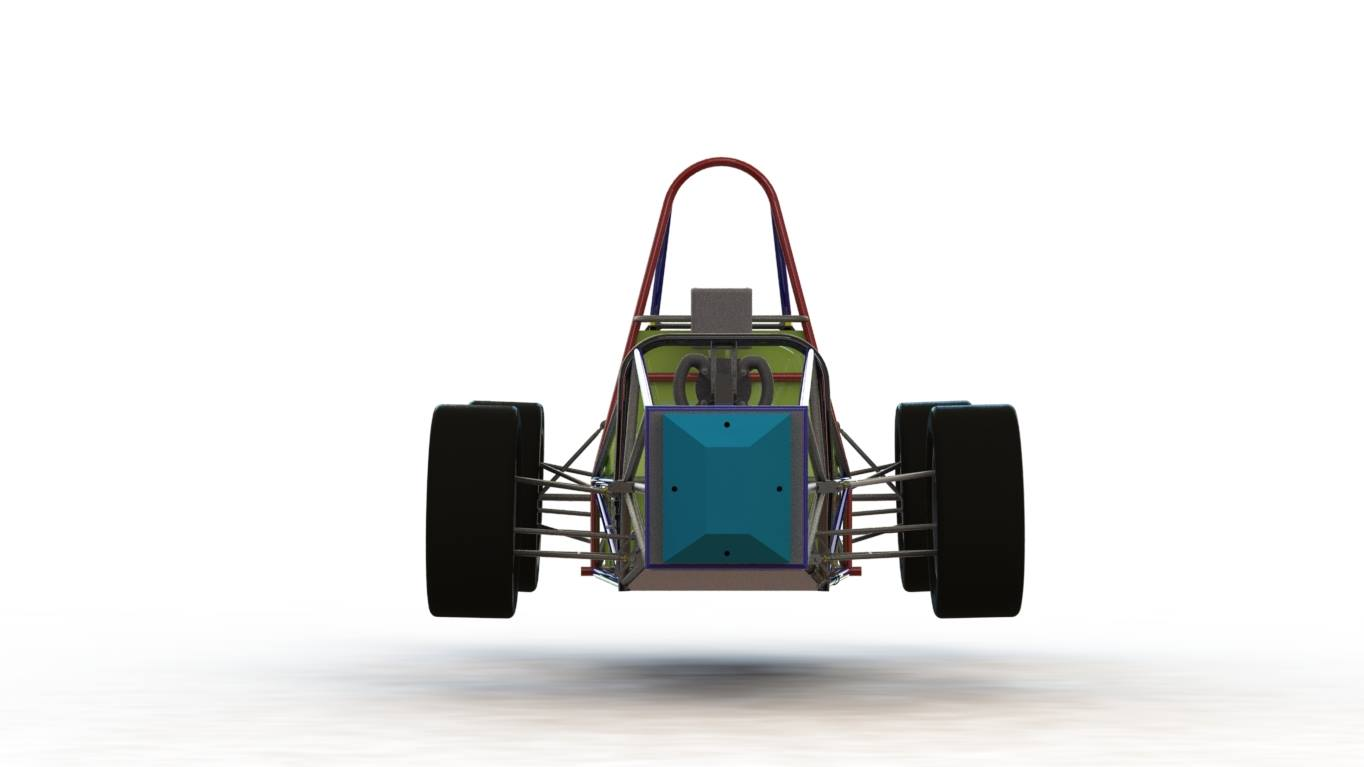
\includegraphics[width = 0.7 \textwidth]{carfront}
            \caption{Full Vehicle, Front View}
            \label{carfront}
        \end{figure}

                \begin{sidewaysfigure}[p]
            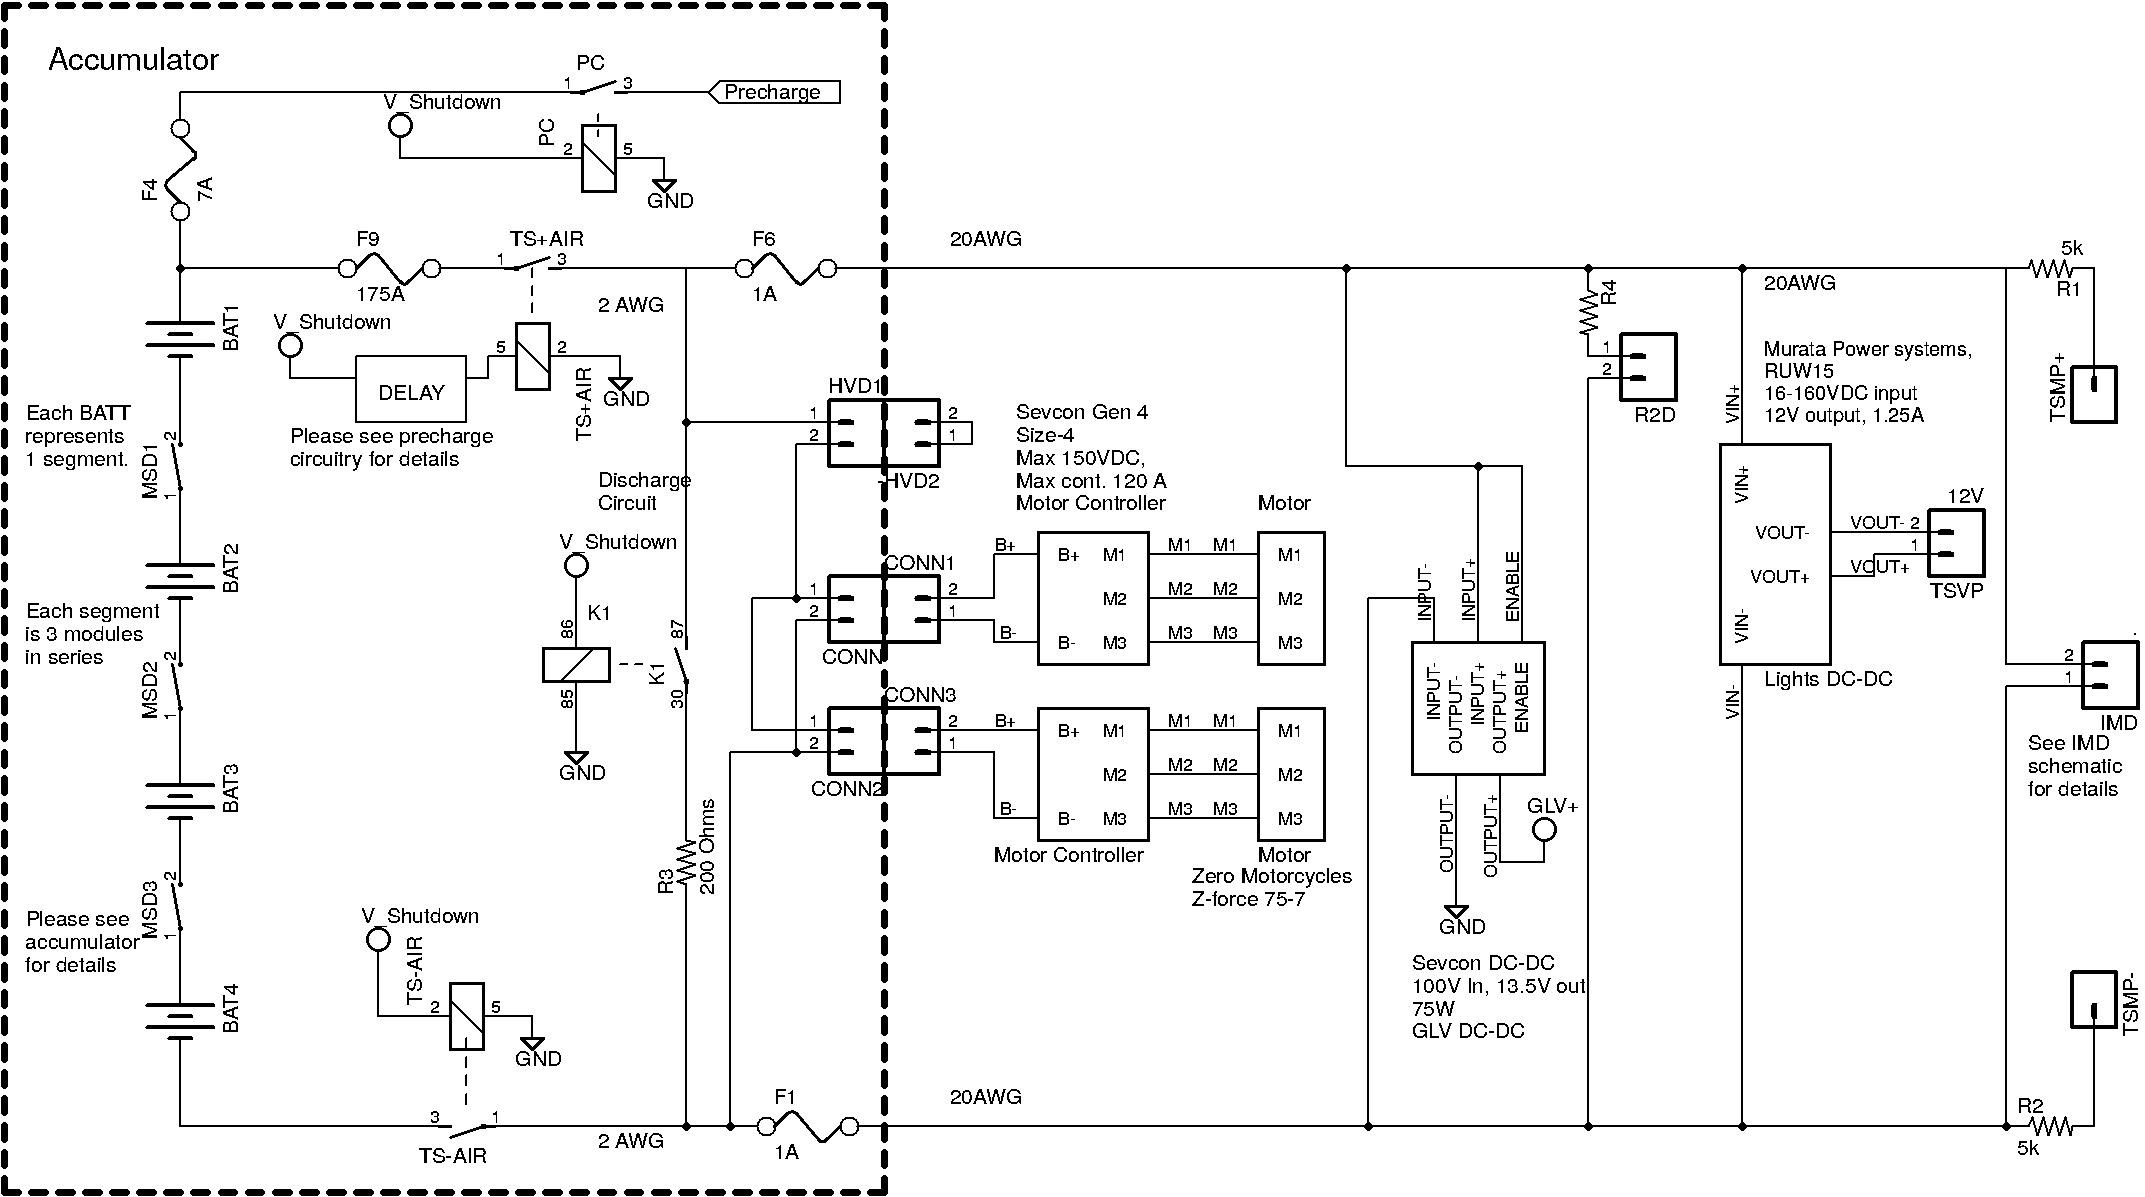
\includegraphics[width=\textheight]{tractiveblock}
            \caption{Tractive system schematic. For wiring of the AMS, please see figure \ref{amsschem}}
            \label{tractiveschem}
        \end{sidewaysfigure}
\newpage

\newpage


%should i include ams or just ams relays?

\textit{Fill in the following table:}

    \begin{table}[H]
        \centering
        \begin{adjustbox}{max width=\textwidth}
        \begin{tabular}{|l|l|}
        \hline
        Item & Data \\ \hline
        Nominal Tractive System Voltage (TSV) & 90 VDC \\ \hline
        Max. TSV (typically this is during charging) & 99.6 VDC \\ \hline
        Control System voltage (GLV) & 12 VDC \\ \hline
        Total Accumulator capacity (Wh) & NDA \\ \hline
        Accumulator Type & Li-ion \\ \hline
        Number of electric motors, total & 2 \\ \hline
        Are wheel motors used? & No \\ \hline
        \end{tabular}
        \end{adjustbox}
        \caption{General Electrical System Parameters}
        \label{generalsystemtable}
    \end{table}

\section{Cables, Fusing \& Grounding}

Person primarily responsible for this section:
    \begin{table}[H]
        \centering
        \label{responsible2}
        \begin{tabular}{lr}
        Name: & Lisa Hachmann \\ \hline
        e-mail: & Lisa.Hachmann@students.olin.edu \\ \hline
        \end{tabular}
    \end{table}

\subsection{Fusing and Overcurrent Protection}

\textit{List TS and GLV fuse (or circuit breaker) data, and where used}
%Fuse table- List TS and GLV fuse (or circuit breaker) data, and where used

    \begin{table}[H]
        \centering
        \begin{adjustbox}{max width=\textwidth}
        \begin{tabular}{|l|l|l|l|l|l|}
        \hline
        Mfg. & \begin{tabular}[c]{@{}l@{}}Fuse Part\\ Number\end{tabular} & \begin{tabular}[c]{@{}l@{}}Cont. \\ Rating (A)\end{tabular} & \begin{tabular}[c]{@{}l@{}}DC Voltage\\ Rating\end{tabular} & \begin{tabular}[c]{@{}l@{}}DC Interrupt\\ Rating (A)\end{tabular} & Where Used \\ \hline
        Bel Fuse & CIQ 3 & 3A & 63V & 63V DC@50A & \begin{tabular}[c]{@{}l@{}}Each input to AMS\\ voltage reading\end{tabular} \\ \hline
        Ferraz Shawmut & A15QS7-2 & 7A & 150V & 100,000 & \begin{tabular}[c]{@{}l@{}}Keyswitch pin \\ activating precharge\end{tabular} \\ \hline
        Bussman & LPJ-175SP & 175A & 300V & 20,000 & \begin{tabular}[c]{@{}l@{}}TS+ before \\ motor controllers\end{tabular} \\ \hline
        Littelfuse & F3169CT-ND & 1A & 125V & 300A@125VDC & \begin{tabular}[c]{@{}l@{}}TS+ low current \\ components, lights' DC-DC \\ converter, \\ GLV DC-DC converter\end{tabular} \\\hline
        Littelfuse & F3169CT-ND & 1A & 125V & 300A@125VDC & \begin{tabular}[c]{@{}l@{}}TS- low current \\ components, lights' DC-DC \\ converter, \\ GLV DC-DC converter\end{tabular} \\\hline
        Littelfuse & MINI2BP & 2A & 32 V & 1000A @ 32 VD & \begin{tabular}[c]{@{}l@{}}12V power, Shutdown circuit. \end{tabular} \\ \hline
        Littelfuse & MINI5BP & 5A & 32 V & 1000A @ 32 VD & \begin{tabular}[c]{@{}l@{}} GLV system \end{tabular} \\ \hline
        Bel Fuse & 0ZCK0050FF2E & 1A & 6V & PTC Resettable & 5V CAN circuit \\ \hline
        \end{tabular}
        \end{adjustbox}
        \caption{Fuse Table}
        \label{fusetable}
    \end{table}

\subsection{Component Fusing}

\textit{List major components (e.g., motor controller, dc-dc converter) and data sheet max fuse rating.  Ensure that the rating of the fuse used is less than the maximum value for the component.}


%Component Fuse Ratings table

\begin{table}[H]
\centering
\begin{adjustbox}{max width=\textwidth}
\begin{tabular}{|l|l|l|l|l|}
\hline
Component & Fuse Part Number & Max Fuse Rating & \begin{tabular}[c]{@{}l@{}}Installed \\ Fuse Rating\end{tabular} & Notes \\ \hline
Motor Controllers & LPJ175sp & 190 A (for 2AWG) & 175A & \begin{tabular}[c]{@{}l@{}}Fused before motor\\ controllers in parallel\end{tabular} \\ \hline
AMS inputs (x28) & CIQ 3 & 4A (for traces) & 3A & \begin{tabular}[c]{@{}l@{}}Each input fused\\ separately\end{tabular} \\ \hline
GLV System & MIN5BP & 7A (for 20AWG) & 5A &  \\ \hline
GLV 12V and Shutdown circuit & MIN2BP & 7A (for 20AWG, traces) & 2A &  \\ \hline
5V CAN circuit & 0ZCK0050FF2E & 1A & 1A &  \\ \hline
\begin{tabular}[c]{@{}l@{}}Lights DC-DC converter, \\ TSMPs and IMD\end{tabular} & F3169CT-ND & 1.25A (for dc-dc converter) & 1A & \begin{tabular}[c]{@{}l@{}}Protects all TS \\ low current\\ components\end{tabular} \\ \hline
\begin{tabular}[c]{@{}l@{}}Keyswitch input to Motor \\ Controller\end{tabular} & A15QS7-2 & \begin{tabular}[c]{@{}l@{}}7A (for motor\\ controller LV input)\end{tabular} & 7A &  \\ \hline
\end{tabular}
\end{adjustbox}
\caption{Component Fuse Ratings}
\label{componenttable}
\end{table}

\subsection{System Wire Tables}

\textit{List wires and cables used in the Tractive System and the GLV system - wires protected by a fuse of 1 A or less may be omitted.
Cable capacity is the value from FH Rules Appendix E (Wire Current Capacity). A revised version of Appendix E that includes metric wire sizes is available at the FH web site. Show available fault current and how calculated. Available fault current can be calculated from FaultCurrent = Vsource / (Rsource + Rwiring)}

%System Wire Table
\begin{table}[H]
\centering
\begin{adjustbox}{max width=\textwidth}
\begin{tabular}{|l|l|l|l|l|l|l|l|l|l|l|l|}
\hline
Mfg & \begin{tabular}[c]{@{}l@{}}Part\\ No\end{tabular} & \begin{tabular}[c]{@{}l@{}}Size \\ AWG\end{tabular} & \begin{tabular}[c]{@{}l@{}}Insulation\\ Type\end{tabular} & \begin{tabular}[c]{@{}l@{}}Voltage\\ Rating\end{tabular} & \begin{tabular}[c]{@{}l@{}}Temp. \\ Rating\end{tabular} & \begin{tabular}[c]{@{}l@{}}Cable\\ Capacity \\ (per FH)\end{tabular} & \begin{tabular}[c]{@{}l@{}}Fuse\\ Part \#\end{tabular} & \begin{tabular}[c]{@{}l@{}}Fuse \\ Cont. A\end{tabular} & \begin{tabular}[c]{@{}l@{}}Fuse Interrupting\\ Rating A\end{tabular} & \begin{tabular}[c]{@{}l@{}}Available\\ Fault Current\end{tabular} & \begin{tabular}[c]{@{}l@{}}Where used \& \\ how fault current\\ is calculated\end{tabular} \\ \hline
Prestolite & \begin{tabular}[c]{@{}l@{}}Not listed\\ UL style 3870\end{tabular} & 2 AWG (33.3 mm\textasciicircum 2) & \begin{tabular}[c]{@{}l@{}}EPDM \\ single layer\end{tabular} & 8 kVAC & 125 C & 190 A & LPJ-175SP & 175 & 20,000 & 41152 A & \begin{tabular}[c]{@{}l@{}}Motor Controllers\\ to Motors x 3, see description\end{tabular} \\ \hline
Delphi & Not listed & 35 mm\textasciicircum 2 & Dual insulated & 600 V & 150 C & $\>190$ A & \begin{tabular}[c]{@{}l@{}}Series\\ with above fuse\end{tabular} & \begin{tabular}[c]{@{}l@{}}See \\ above\end{tabular} & See above & 41152 A & \begin{tabular}[c]{@{}l@{}}Accumulator to\\ HVD, Accumulator\\ to Motor controllers x2\end{tabular} \\ \hline
Wiechang & Unknown & See below & XLPE & 600V & 150 C & Motor leads & Series with above fuse & See above & See above  & 41152 A & See description \\ \hline
CnC Tech & 3132-20-1-0500-001-1-TS & 20 AWG & Silicone Rubber & 300V & 150 C & 7 A & MIN2BP & 5A & 25 $A^{2}s$ & 25A & See description \\ \hline
\end{tabular}
\end{adjustbox}
\caption{System wire table}
\label{systemwiretable}
\end{table}

The motor leads are permanently attached by the manufacturer, and are OEM. The width of the motor lead with insulation (other measurements cannot be taken) is 0.45 inch, so we believe it to be of at least 2 AWG.

The fault current for the motor to motor controller wiring (Prestolite), is calculated as follows (using FH-supplied formula):

\begin{align}
    \text{Fault Current} = \dfrac{V_{source}}{R_{source} + R_{wiring}}\\
    \text{Fault Current} = \dfrac{100}{0.00149 \ohm + 0.00094 \ohm}\\
    \text{Fault Current} = 41152 A
\end{align}

The fault current for the accumulator to motor controller wiring (Delphi), is calculated as follows (using FH-supplied formula):

\begin{align}
    \text{Fault Current} = \dfrac{V_{source}}{R_{source} + R_{wiring}}\\
    \text{Fault Current} = \dfrac{100}{0.00149 \ohm + 0.00145 \ohm}\\
    \text{Fault Current} = 34013 A
\end{align}

The fault current for the GLV system is restricted by the DC-DC converter supplying power to the GLV system. The DC-DC converter can only output 25A, and will restrict any fault current to 25A.

\subsection{Grounding System}

\textit{Describe how you keep the resistances between accessible components below the required levels as defined in FH Rules EV4.3. If wire is used for ground bonding, state the AWG or mm2 of the wire}

The chassis is used as GLV ground. This ground is established at the side panel mount holding many of the shutdown components and the TSMP's. All mechanical systems in the vehicle, such as the accumulator, drivers seat, and pedal box, achieve low resistance to ground because they are either welded directly to the chassis, or fastened using uncoated, conductive metal fasteners. Electrical systems that are satellite to the main panel mount that need to establish a connection to ground for sense purposes are grounded to the chassis using ring terminals. Ring terminals can be included in the bolt stack up of mechanical systems to ensure a secure connection to ground that is positively retained with a lock nut. All wires used for ground bonding will be 20 AWG, which is the same wire gauge as the GLV system. During charging, there will be a green 16 AWG wire connecting the GLV system to earth ground.


\subsection{Conductive Panel Grounding}

\textit{If carbon fiber or coated conductive panels are used in your design, describe the fabrication methods used to ensure point to point resistances that comply with EV4.3.2. Describe results of measurements made per EV4.3.3.}

We are not using CFRP or conductive materials in our vehicle.

\section{Isolation and Insulation}
Person primarily responsible for this section:
    \begin{table}[H]
        \centering
        \label{responsible3}
        \begin{tabular}{lr}
        Name: & Lisa Hachmann \\ \hline
        e-mail: & Lisa.Hachmann@students.olin.edu \\ \hline
        \end{tabular}
    \end{table}

%%%%%%%%%%%%%%%%%%%%%%%%%%%%%%%%%%%%%SECTION 3 %%%%%%%%%%%%%%%%%%%%%%%%%%%%%%%%%%%%%%%%%%%%%%%%%%%%%%%%%%%%%%%%%%%%%%%%%%
    \subsection{Separation of Tractive System and Grounded Low Voltage System}

\textit{Describe how the TS and GLV systems are physically separated (EV4.1). Add CAD drawings or photographs of how TS and GLV are segregated in key areas of the electrical system.}

%figures of ts and glv separation

\textit{List all electrical circuit boards designed by team that contain TS and GLV voltage in the following table.}

%table of PCB spacings

% The second table should include any component, in your AMS or otherwise, that is connected
% to both the Tractive and the GLV system. You should add in the "Notes" column the general
% location of these parts. The spacing table allows us to reference the boards that have TS
% and GLV in close proximity, and the parts table allows us to reference the data sheets of
% the parts that span the gap the spacing creates.

\begin{table}[H]
\centering
\begin{adjustbox}{max width=\textwidth}
\begin{tabular}{|l|l|l|l|l|}
\hline
Device/PCB & TS Voltage Present & \begin{tabular}[c]{@{}l@{}}Minimum \\ Spacing mm\end{tabular} & \begin{tabular}[c]{@{}l@{}}Thru Air or\\ Over surface\end{tabular} & Notes \\ \hline
\begin{tabular}[c]{@{}l@{}}AIR Control Board \\ (Precharge, Discharge,\\ Lights, AMS relays, etc)\end{tabular} & 100 V & 6.4 & Over Surface &  \\ \hline
\begin{tabular}[c]{@{}l@{}}Accumulator Management\\  System (x4)\end{tabular} & 100V & 6.4 & Over surface & \begin{tabular}[c]{@{}l@{}}1 AMS per segment, \\ each segment nominally\\ 22.5V\end{tabular} \\ \hline
\begin{tabular}[c]{@{}l@{}}Side Panel CAN node \\ (Ready to drive sound, TSMP)\end{tabular} & 22.5V & 6.4mm  & Over Surface &  \\ \hline
Motor Controller Isolation & 100 V & 6.4 & Over surface &  \\ \hline
\end{tabular}
\end{adjustbox}
\caption{PCB Spacings}
\label{pcbspacingstable}
\end{table}

\textit{Add a figure (board layout drawing) for each team-designed PCB showing that spacings comply with EV4.1.8.}

%figures of each row

\begin{figure}[H]
    \centering
    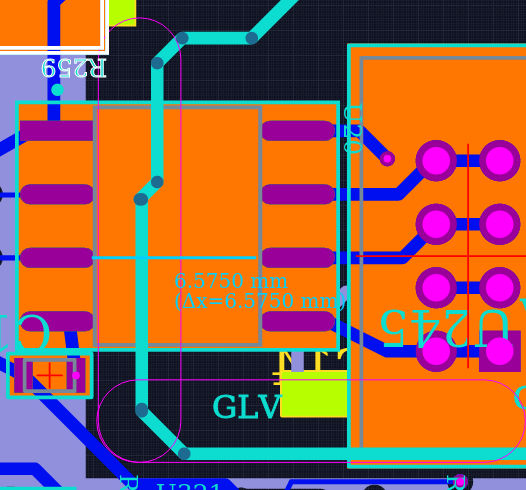
\includegraphics[width = 0.6 \textwidth]{bms_separation}
    \caption{Capture of the separation on each AMS board between TS and GLV power (6.57 mm)}
    \label{amsseparation}
\end{figure}

\begin{figure}[H]
    \centering
    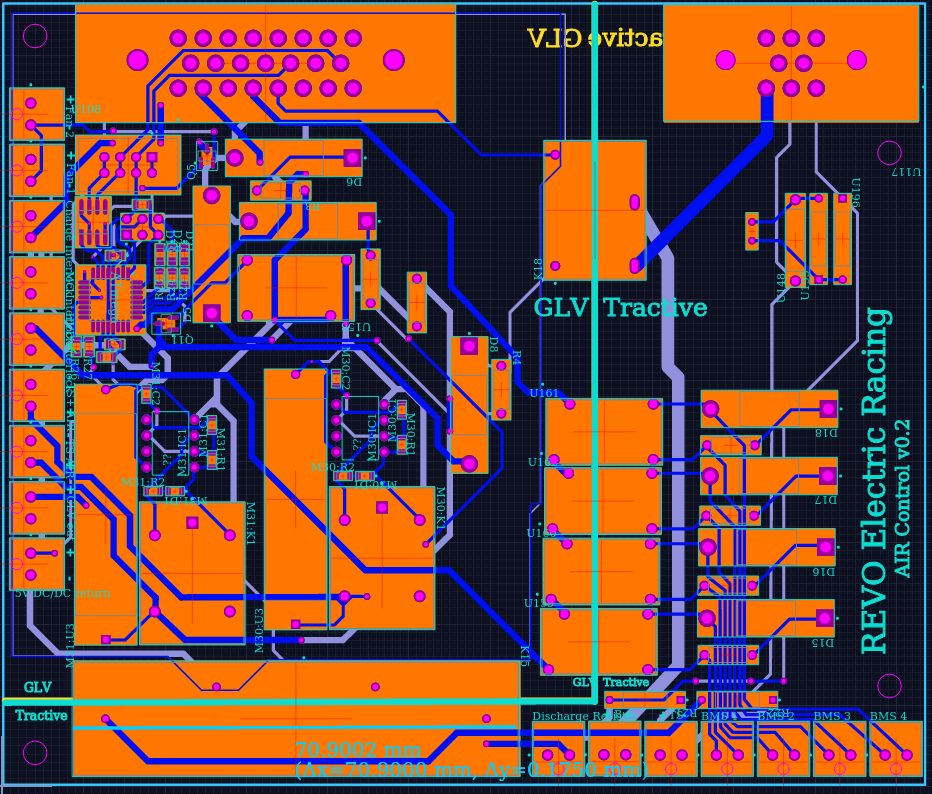
\includegraphics[width = 0.6 \textwidth]{aircntrlCAD}
    \caption{AIR control board, with the bright blue line denoting the separation between the TS and GLV voltage. The smallest separation is 8.5 mm (over surface)}
    \label{AIRcontrolspacing}
\end{figure}

\begin{figure}[H]
    \centering
    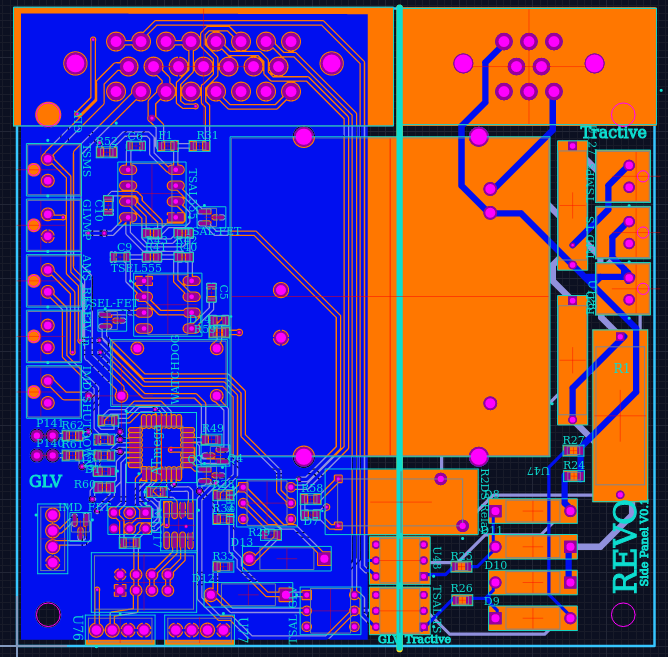
\includegraphics[width = 0.7 \textwidth]{sidepanelPCB}
    \caption{Side Panel board, with the bright blue line denoting the separation between the TS and GLV voltage. The smallest separation is 1/4 in (over surface)}
    \label{sidepanelspacing}
\end{figure}

\begin{figure}[H]
    \centering
    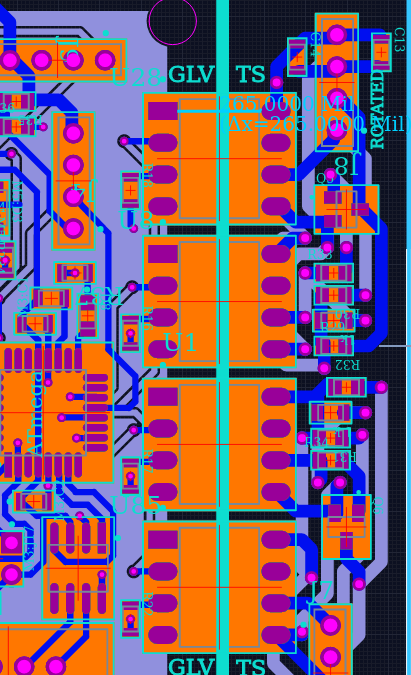
\includegraphics[width = 0.6 \textwidth]{MCCspacing}
    \caption{Motor Controller Isolation board, which has a bright blue line denoting the separation between the TS and GLV voltage. The spacing is 6.731 mm. consistently (over surface)}
    \label{MCCspacing}
\end{figure}

\textit{List all purchased components with both TS and GLV connections (at min motor controller and AMS).}

\begin{table}[H]
\centering
\begin{adjustbox}{max width=\textwidth}
\begin{tabular}{|l|l|l|l|}
\hline
Component & Isolation method & \begin{tabular}[c]{@{}l@{}}Link to Document\\ Describing Isolation\end{tabular} & Notes \\ \hline
Precharge relay & Galvanic (relay) & \href{http://www.mouser.com/ds/2/307/G5LE\_0813-267607.pdf}{Click here} &  \\ \hline
Discharge relay & Galvanic (relay) & \href{http://cotorelay.com/wp-content/uploads/2014/09/5500\_series\_reed\_relay\_datasheet.pdf}{Click Here} &  \\ \hline
GLV DC-DC converter & Not listed & \href{http://www.evdrives.com/product\_p/vr-sevcon-7213.htm}{Click Here} &  \\ \hline
Lights DC-DC converter & \begin{tabular}[c]{@{}l@{}}Not listed: Isolation\\ test at 5000V\end{tabular} & \href{http://www.mouser.com/ds/2/281/mdc\_ruw15-217876.pdf}{Click Here} &  \\ \hline
Ready to drive relay & Galvanic (relay) & \href{http://pdf1.alldatasheet.com/datasheet-pdf/view/451822/MACOM/SDT-S-124DMR000.html}{Click Here} &  \\ \hline
AMS relay x4 & Galvanic (relay) & \href{http://www.te.com/commerce/DocumentDelivery/DDEController?Action=srchrtrv\&DocNm=OJ\_OJE\_series\_relay\_data\_sheet\_E\&DocType=DS\&DocLang=English}{Click Here} &  \\ \hline
Photorelay mosfet & Galvanic (Photorelay) & \href{http://toshiba.semicon-storage.com/info/docget.jsp?did=17083\&amp;prodName=TLP592A}{Click Here} &  \\ \hline
Isolated CAN Tranceiver & Galvanic & \href{http://www.ti.com/lit/ds/symlink/iso1050.pdf}{Click Here} &  \\ \hline
BSPD Relay & None listed & \href{http://www.mouser.com/ProductDetail/TE-Connectivity/OJ-SH-105HM000/?qs=%2fha2pyFaduihBgI7ARjI70jHf%2f4%2fFPQxhir8DUrpU%252bkAVAYrW5DJOg%3d%3d}{Click Here} &  \\ \hline
\end{tabular}
\end{adjustbox}
\caption{Purchased Components - Isolation Data}
\label{purchased-isolationtable}
\end{table}

%Weirdly unnamed table, about component and isolation

\subsection{Isolation and Insulation}

\textit{Provide a list of containers that have TS and GLV wiring in them. If a barrier is used rather than spacing, identify barrier material used (reference Table 7- Insulating Materials).}

\begin{table}[ht]
\centering
% \caption{My caption}
% \label{my-label}
\begin{adjustbox}{max width=\textwidth}
\begin{tabular}{|l|r|l|l|l|l|}
\hline
Container Name & Segregation by Spacing (Y or N) & \begin{tabular}[c]{@{}l@{}}How\\   is spacing maintained?\end{tabular} & \begin{tabular}[c]{@{}l@{}}Actual\\   Measured Spacing mm\end{tabular} & Alt,– Barrier Material P/N & Notes \\ \hline
Accumulator Container & Y & Kevlar reinforced nylon cable clips and cable ties &  &  Mcmaster 8667K55 (Garolite) & Garolite is also used as the barrier between segments, TS fuse and, AIRs. Accumulator is in assembly so measured distance is unavailable. \\ \hline
TSMP Housing & Y & Kevlar reinforced nylon cable clips and cable ties &  &  & \begin{tabular}[c]{@{}l@{}}This part is also in assembly \\ eso the measured spacing is not\\ finalized yet. \end{tabular}    \\ \hline
\end{tabular}
\end{adjustbox}
\end{table}

\textit{List all insulating barrier materials used to meet the requirements of EV1.3 or EV4.1.5}
\begin{table}[ht]
\centering
% \caption{My caption}
% \label{my-label}
\begin{adjustbox}{max width=\textwidth}
\begin{tabular}{|l|l|l|l|l|}
\hline
Insulating Material / Part Number & UL Recognized ? & Rated Temperature ºC & Thickness mm & Notes \\ \hline
N/A & N/A & N/A & N/A & N/A \\ \hline
\end{tabular}
\end{adjustbox}
\end{table}

\subsection{Conduit}

\textit{List different types of conduit used in the design. Specify location and if manufacturer’s standard fittings are used. Note Virtual Accumulator Housing FH Rules EV3.3.1 requires METALLIC type LFMC.}

\textit{Describe how the conduit is anchored if standard fittings are not used.}

%table of Conduit Data
\begin{table}[H]
\centering
\begin{tabular}{|l|l|l|l|l|l|}
\hline
\begin{tabular}[c]{@{}l@{}}Conduit \\ Type\end{tabular} & MFR & Part Number & Diameter & \begin{tabular}[c]{@{}l@{}}Standard\\ fittings\end{tabular} & Location/Use \\ \hline
PVC Nylon PVC & N/A (McMaster) & 8465K23 & \begin{tabular}[c]{@{}l@{}}3/4" trade\\ size\end{tabular} & Y & \begin{tabular}[c]{@{}l@{}}Motor to Motor\\ controller (x2)\end{tabular} \\ \hline
\end{tabular}
\caption{Conduit Data}
\label{conduittable}
\end{table}

\textit{Is all conduit contained within the vehicle Surface Envelope per EV4.2.1? (Y or N).}

Yes, all conduit is contained within the vehicle surface envelope per EV4.2.1.

\textit{Does all conduit comply with EV4.5.10? (Y or N).}

Yes all conduit complies with EV4.5.10.

\subsection{Shielded Dual-Insulated Cable}

\textit{If shielded, dual-insulated cable per EV4.5.8 used in the vehicle, provide specifications and where used:}

%table of Shielded Dual Insulated Cable Data
\begin{table}[H]
\centering
\begin{tabular}{|l|l|l|l|l|}
\hline
MFR & \begin{tabular}[c]{@{}l@{}}Part \\ Number\end{tabular} & Cross section & \begin{tabular}[c]{@{}l@{}}Shielded \\ ground at\end{tabular} & Location/Use \\ \hline
Delphi & Unknown & 35 mm\textasciicircum 2 & Y & \begin{tabular}[c]{@{}l@{}}Accumulator to HVD, \\ Accumulator to Motor \\ controllers (x2)\end{tabular} \\ \hline
\end{tabular}
\caption{Shielded Dual Insulated Cable Data}
\label{shieldedwiretable}
\end{table}

The Delphi shielded cable is being provided by General Motors, and we are still trying to get the part number at this time.

\subsection{Firewall(s)}

\textit{Describe the concept, layer structure and the materials used for the firewalls. Describe how all firewall requirements in FH Rules T4.5.1 are satisfied. Show how the low resistance connection to chassis ground is achieved.}

\textbf{Description/Materials}

            The firewall is constructed of two layers. The layer facing the tractive system is 1.5 mm aluminum sheet metal, with a chamfered edge. The second layer facing the cockpit is 1/8 in. Flame-Retardant Multipurpose Garolite (G-10/FR4). The assembly is fastened together using sheet metal rivets. The chassis has welded sheet metal tabs that fasten to the firewall with bolts and positively retained nuts. Because the firewall is fastened to the chassis using conductive fasteners, it is connected to GLVS ground.\\

            All high voltage and high temperature systems are contained in the rear of the vehicle, so only one firewall will be used. There are GLV systems in the dashboard and pedal box. A small grommeted hole will be made in the firewall for GLV wiring only.

            %this is not the latest version of the firewall (exploded).

            \begin{figure}[H]
                \centering
                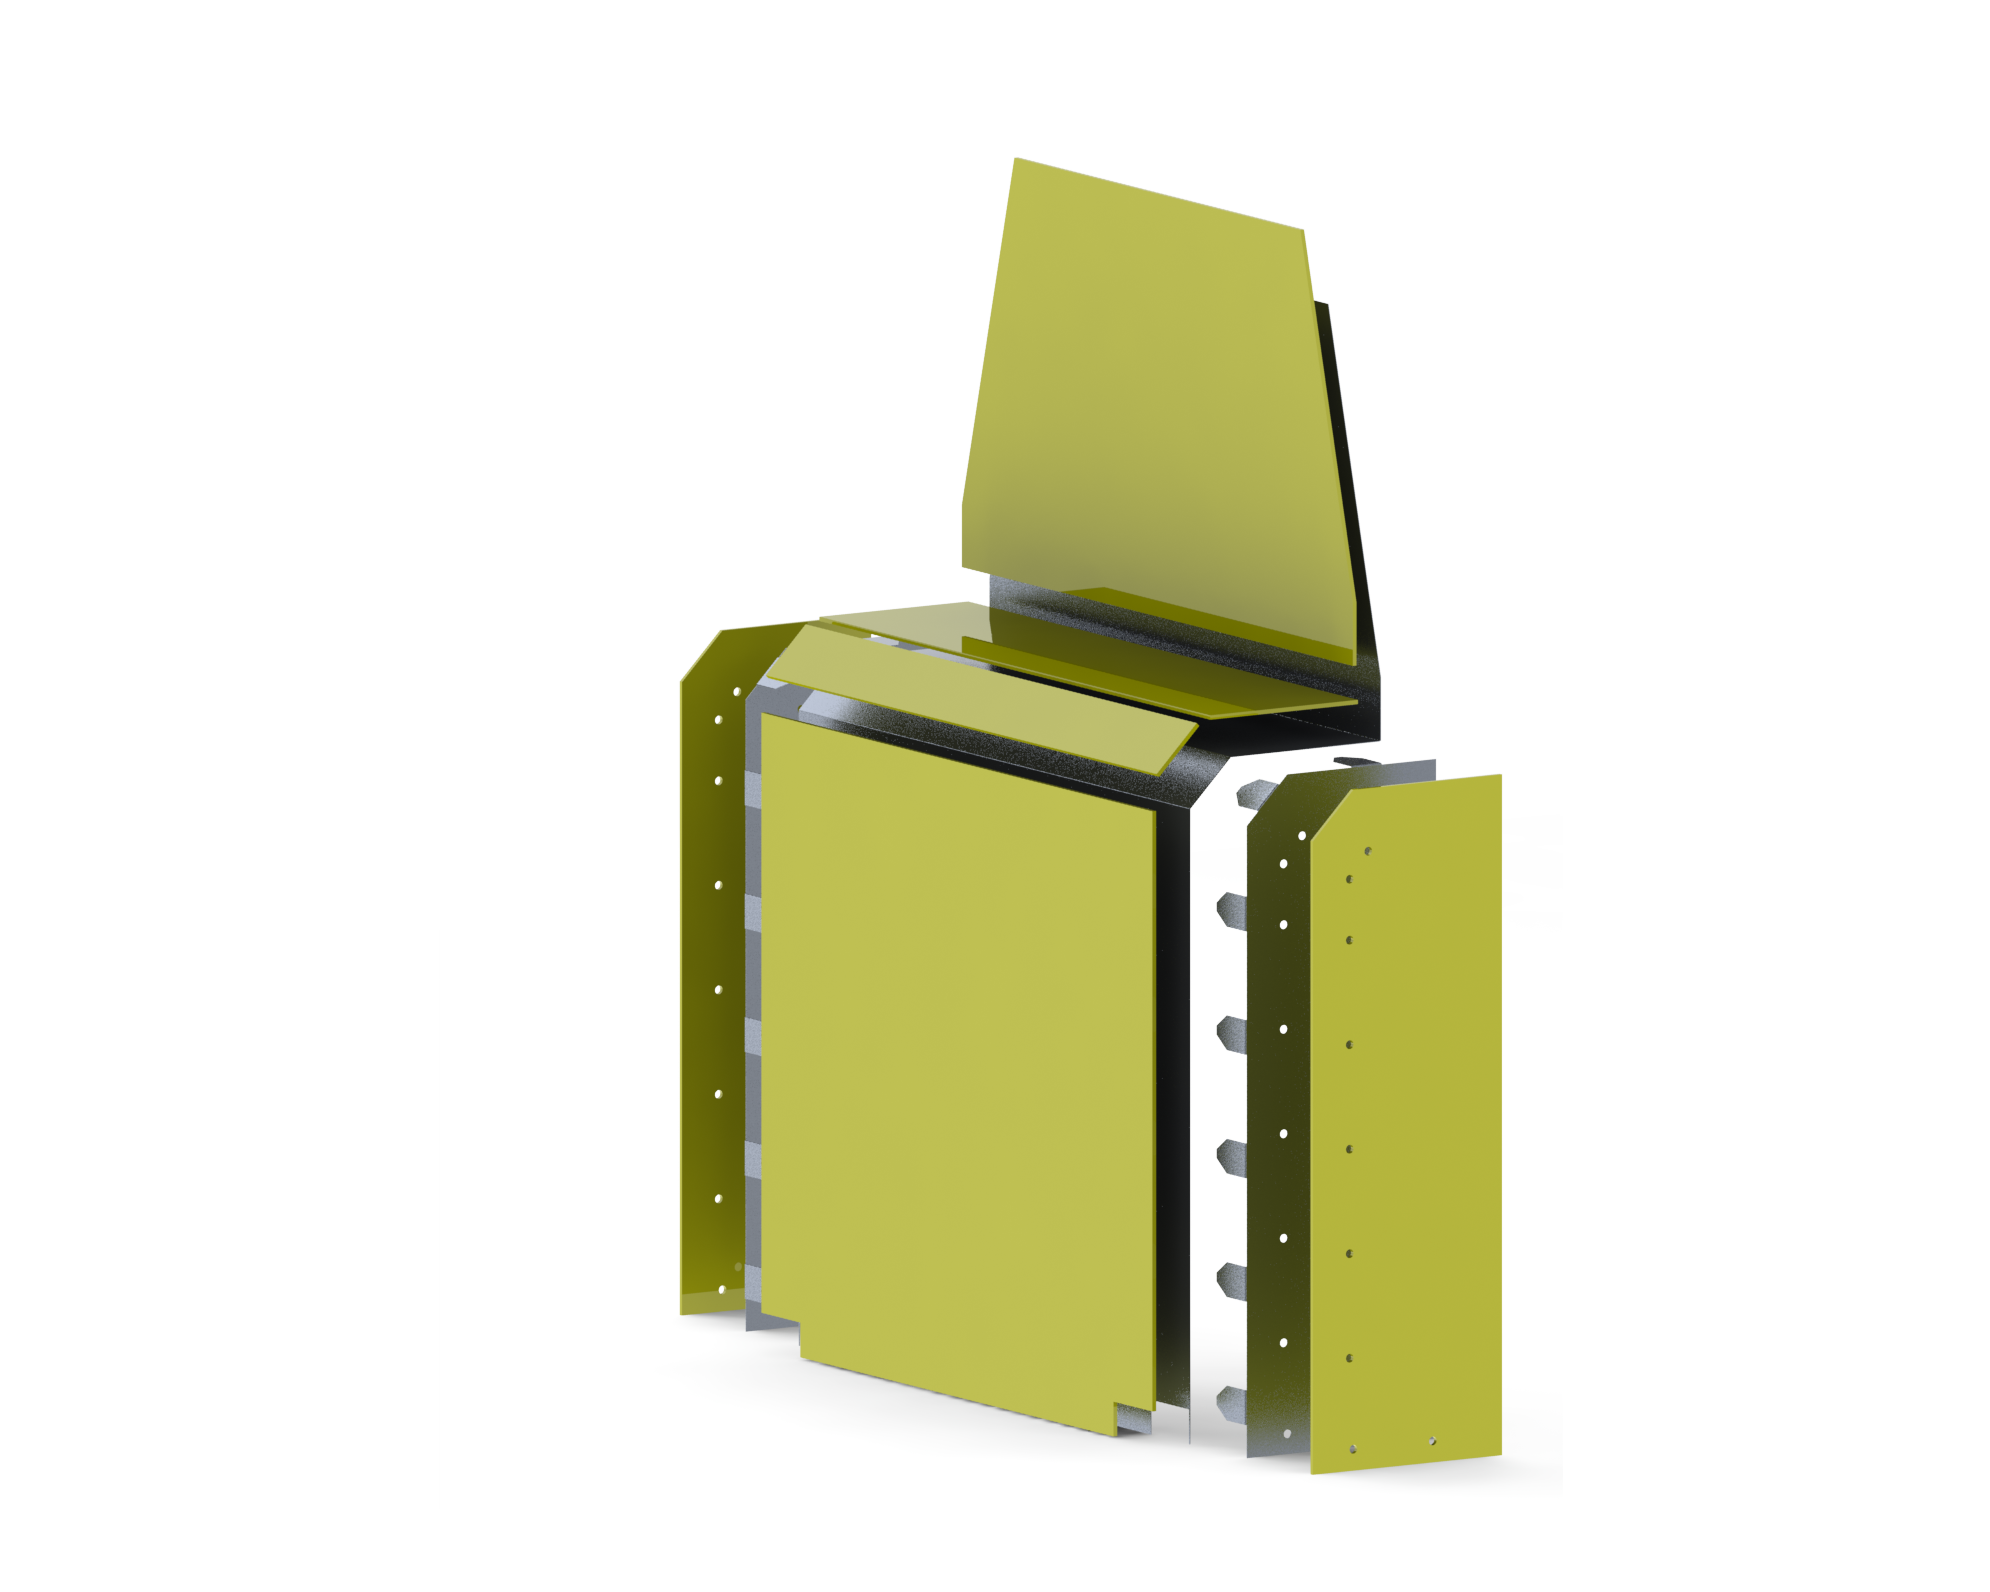
\includegraphics[width = 0.6 \textwidth]{ExplodedView}
                \caption{Exploded view of the firewall}
                \label{explodedfirewall}
            \end{figure}

\textbf{Position in Car}

\textit{Provide CAD-rendering or photographs showing the location of the firewall(s)}

            The firewall is located between the driver and the accumulator, to protect the driver from the TS. Figure \ref{firewallposition} shows the position with the driver seat. The top corner of the extruded part of the firewall is chamfered in order to protect the driver and will also be covered with padding.

            \begin{figure}[H]
                \centering
                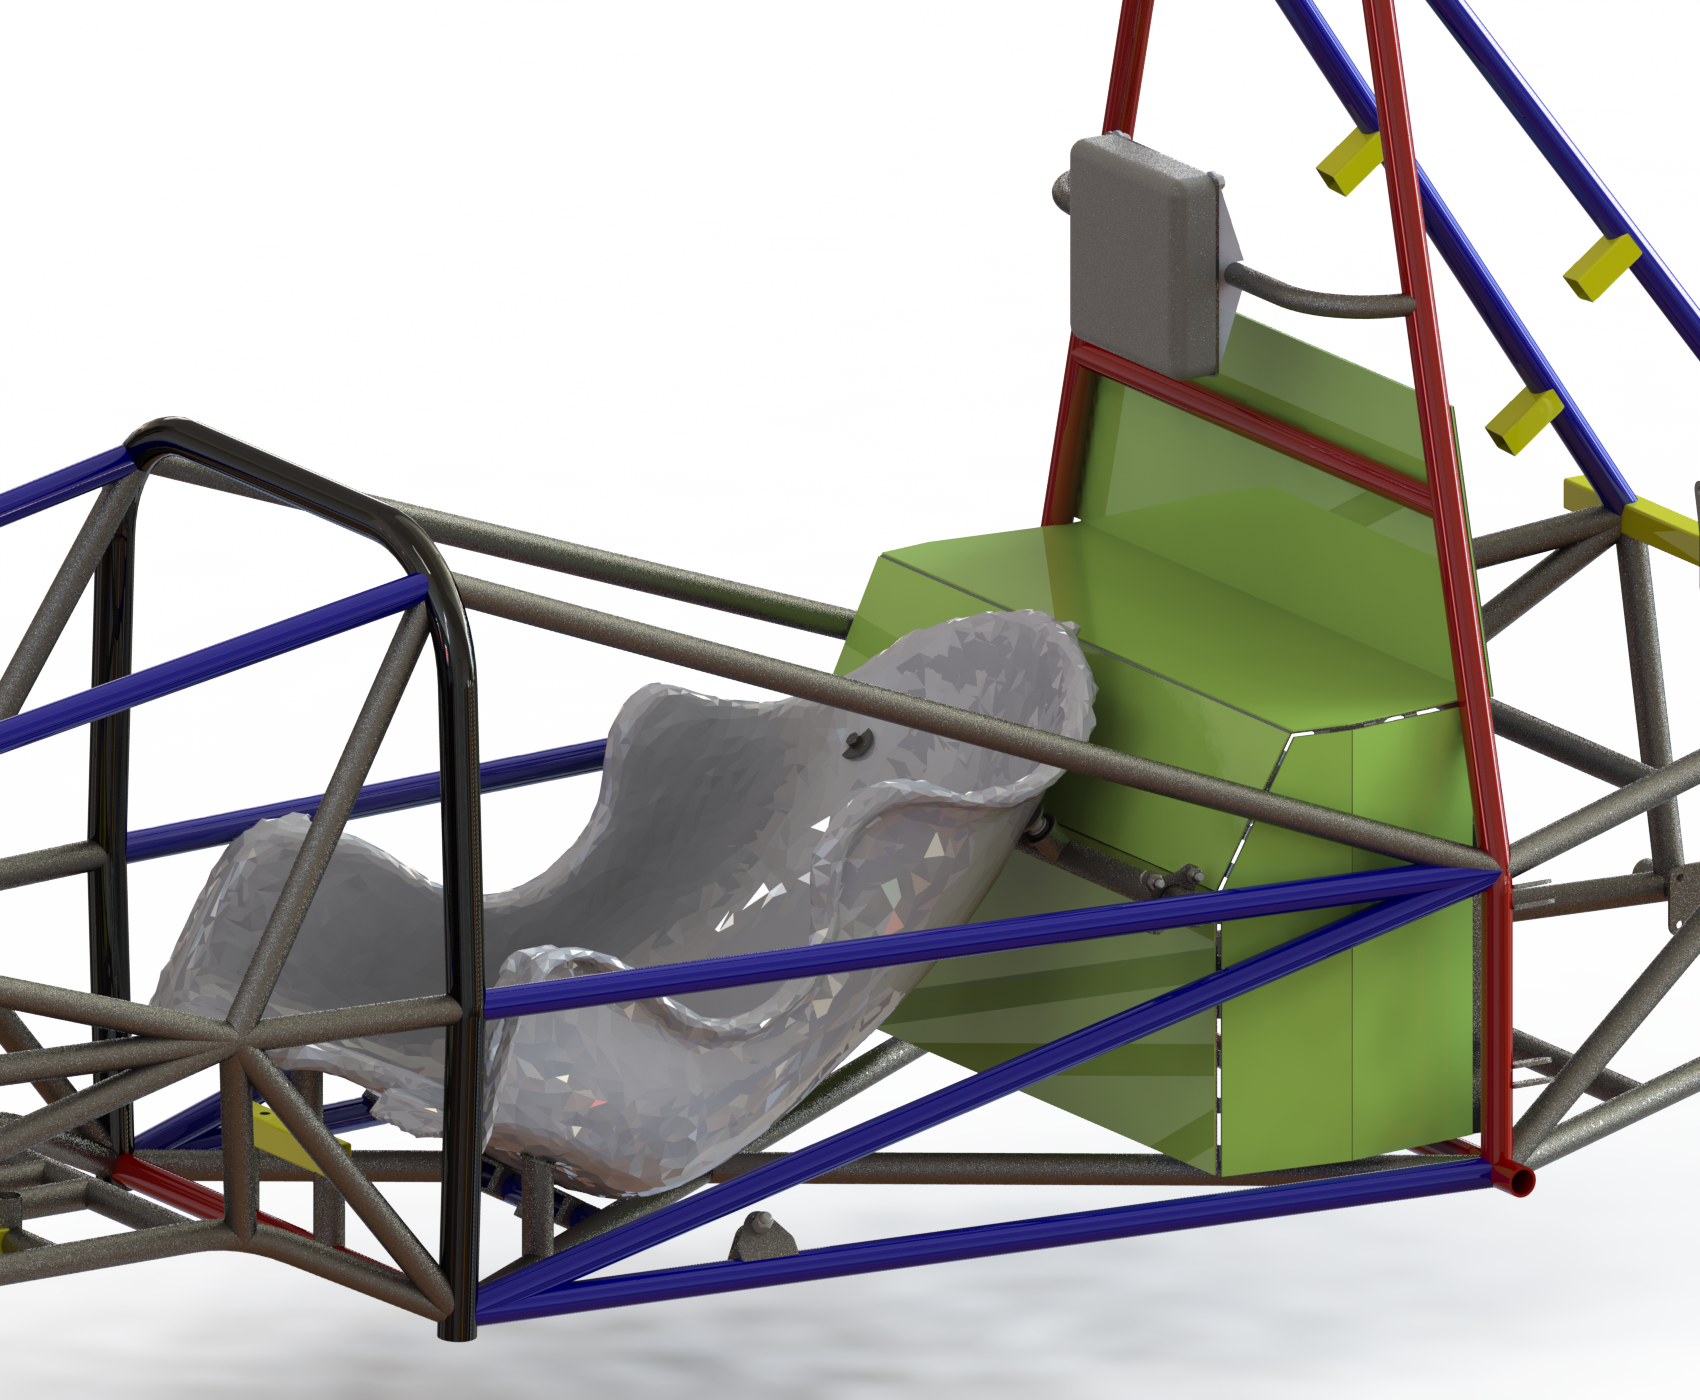
\includegraphics[width = 0.65 \textwidth]{FullCar2_13_16}
                \caption{CAD render of the firewall's position in the car}
                \label{firewallposition}
            \end{figure}

%%%%%%%%%%%%%%%%%%%%%%%%%%%%%%%%%%%%%%%%%%%%%%%%%%%%%%%%%%%%%%%%%%%%%%%%%%%%%%%%%%%SECTION 4%%%%%%%%%%%%%%%%%%%%%%%%%%%%%%%%%%%%%%%%%%%%%%%%%%%%%%%%%%%%%%%%%%%%%%%%%%%%%%%%%%
\section{Electric Tractive System}
Person primarily responsible for this section:
    \begin{table}[H]
        \centering
        \label{responsible4}
        \begin{tabular}{lr}
        Name: & Lisa Hachmann \\ \hline
        e-mail: & Lisa.Hachmann@students.olin.edu \\ \hline
        \end{tabular}
    \end{table}

    \subsection{Motor(s)} \label{mcurrent}

    \textit{Describe the motor(s) used and reason for this particular choice. Add additional tables if multiple motor types are used}

    The motors used are Zero Motorcycles Z-Force 75-5 BLDC motors, which are manufactured and used by Zero Motorcycles in their production units. We have an established sponsorship with Zero Motorcycles, which is the primary reason for our motor selection. The motors are paired to two Sevcon Gen 4 Size 4 motor controllers, which are also used in Zero's production units.

    \begin{table}[H]
        \centering
        \begin{tabular}{|l|l|}
            \hline
            Manufacturer and Model & \begin{tabular}[c]{@{}l@{}}Zero Motorcycles,\\  Model \# 30-0534\end{tabular} \\ \hline
            Motor type & DC Brushless \\ \hline
            Number of motors of this type used & 2 \\ \hline
            Nominal motor voltage (Vdc) & 104  Vdc \\ \hline
            Nominal/Peak motor current (A) & Nom: 250 / Peak: 420 \\ \hline
            Nominal/Peak motor power & Nom: 24.9  / Peak: 41.8\\ \hline
            Motor wiring - conductor size and type &  $\geq$ 2 $AWG$\\ \hline
        \end{tabular}
        \caption{Motor Data}
        \label{motortable}
    \end{table}

    The motor wiring (Weicheng) is permanently attached and grommetted to the motor casing. The wire gauge was measured to be 0.45 inches with single-layer XLPE insulation, so we believe the wire gauge to be greater to or equal to 2 AWG. 2AWG wire from Panduit with single-layer thermoplastic insulation is specified to have an outside diameter of 0.420 inches, less than the measured outside diameter of the motor leads.

    \textit{Provide calculations for currents and voltages. State how this relates to the choice of cables and connectors used.}

    The choice of cables and connectors were made in reverse from the motor's maximum current draw. With the maximum current draw for 10 seconds being 660A (at 100V) for both motors combined, we specified the smallest fuse rated for that amount of current draw: 175A continuous. For a 175A fuse, the smallest wire gauge specified from Appendix E of the rules is 2 AWG (rated up to 190A). All wire gauges and connectors specified for the motors and/or accumulator are equal to or greater than 2 AWG.

    \subsection{Motor Controller}

    \textit{Describe the motor controller(s) used and reason for this particular choice. Add additional tables if multiple motor controller types are used.}

    The motor controllers were chosen because they pair well with the chosen motors, and they can be controlled by either CAN or analog signals.

    % \begin{table}[H]
    \begin{table}[htbp]

    \centering
    \setlength\tabcolsep{2pt}
    \begin{tabular}{|l|l|}
        \hline
        Manufacturer and Model & Sevcon Size 4 Gen 4 \\ \hline [-3pt]
        Number of controllers of this type used & 2 \\ \hline
        Maximum Input voltage (Vdc) & 116 VDC \\ \hline
        Nominal Input current (A) & 350 A \\ \hline
        Max Input Fuse (A) per Mfr. & 355 A \\ \hline
        Output Voltage (Vdc) & Same as input voltage \\ \hline
        \begin{tabular}[c]{@{}l@{}}Isolation rating between GLV \\ (power supply or control inputs) and\\  TS connections\end{tabular} & None \\ \hline
        %\begin{tabular}[c]{@{}l@{}}Is the accelerator galvanically \\ isolated from the Tractive system per EV2.3\end{tabular} & No \\ \hline
        \begin{tabular}[c]{@{}l@{}}Is the accelerator galvanically \\ isolated from the Tractive system per EV2.3\end{tabular} & Yes \\ \hline
    \end{tabular}
    \caption{Motor Controller Data}
    \label{mctable}
    \end{table}

    \textit{If the answer to the last question is NO, how to you intend to comply with rule EV2.3 (an external isolator is acceptable)}


    %%%%% Our throttle is galvanically isolated from the TS. No need for clarification.

    %\textcolor{red}{We will have isolation on our accelerator (throttle pedal potentiometers) by isolated CAN transceivers. Although we currently do not control the motor controller through CAN messages, we have a node next to the motor controller that listens to the throttle's data and outputs the same (isolated) analog signal. The only use of the CAN system with the throttle information is logging the data for the team's use. The throttle information is not altered in any way. }

    \textit{Provide calculations for currents and voltages. State how this relates to the choice of cables and connectors used.}

    Please see section \ref{mcurrent}, as the same choices were made between motors and motor controllers.

    \subsection{Tractive System Measurement Points (TSMP)}

    \textit{The TSMP must comply with FH Rule EV4.4. Describe the TSMP housing and location. Describe TSMP electrical connection point.}

    The TSMP housing is a kevlar-reinforced nylon 3-D printed enclosure that is located in the rear right side of the car, behind the main hoop. This housing also contains most of the shutdown components. Electrically, it is connected to the TS+ and TS- power lines (past the AIR's, in a separate connector and wiring bundle), in parallel to the motors. The housing includes all low-current TS voltage components. Please see Figure \ref{tractiveschem} for the schematic in the larger context, as Figure \ref{tsmpschem} is a schematic focused on the TSMPs, with and without the multimeter.

    \begin{figure}
        \centering
        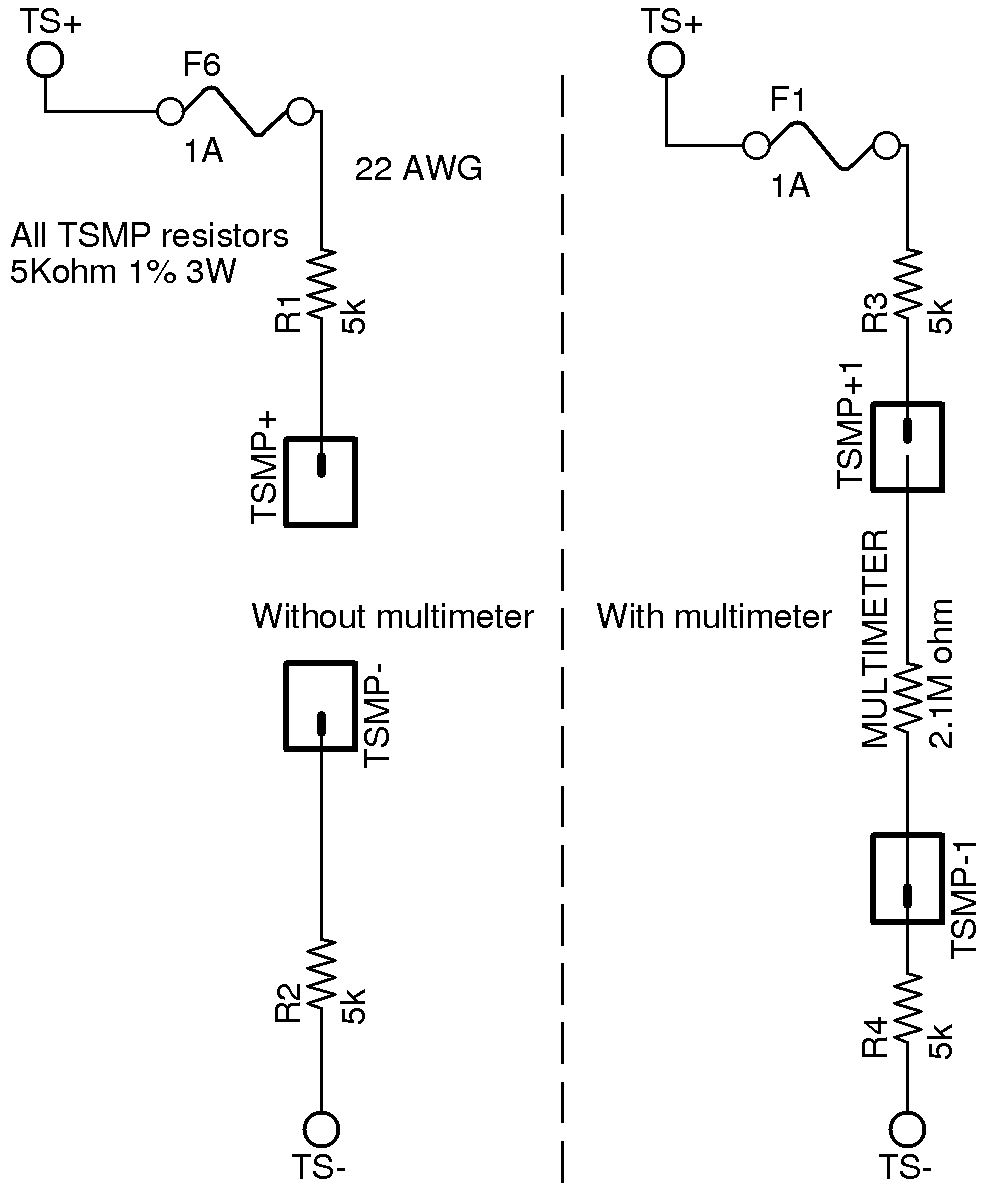
\includegraphics{TSMP}
        \caption{TSMP Schematic, with and without multimeter probes.}
        \label{tsmpschem}
    \end{figure}

    The TSMP resistors follow the following calculations:

                \begin{align}
                V = I * R \\
                100 V = I * 10,000 \ohm \\
                I = 0.01A
            \end{align}

            \begin{align}
                P = I * V \\
                P = 0.01 I * 100V V \\
                P = 1 W
            \end{align}

            Therefore, a 1W, 5k\ohm resistor will be placed before each TSMP banana jack. The resistor will be on a small, separate PCB or break out board that only contains the resistors to the TSMPs. This PCB does not have a finished design yet, but will be housed such that it is insulated from all adjacent conductive materials.\\

            Another worst case scenario that could occur at the measuring points is a short between the TS and GLV systems over the banana jacks, again by operator error. In this scenario, the IMD will open the shutdown circuit.
    \\
    The following figures show the housing for the TSMP's and shutdown components:

    \begin{figure}[H]
        \centering
        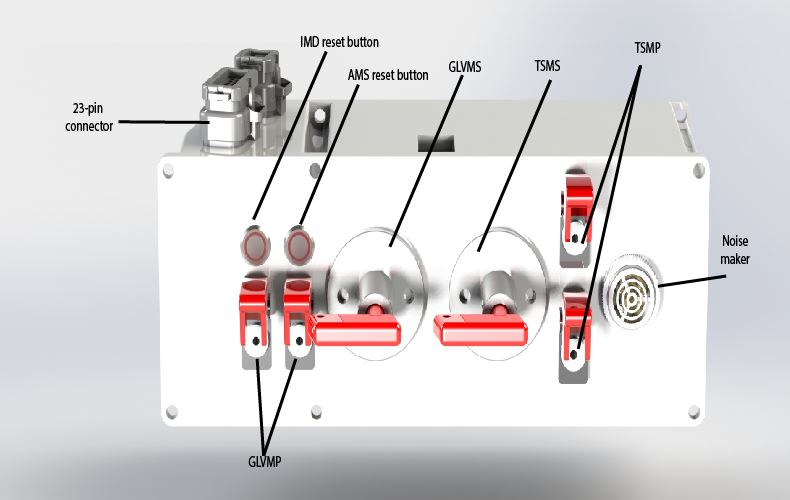
\includegraphics[width = 0.6 \textwidth]{CONTROLPANEL_1}
        \caption{TSMP Housing Vehicle Location}
        \label{tsmplocation}
    \end{figure}

    \begin{figure}[H]
        \centering
        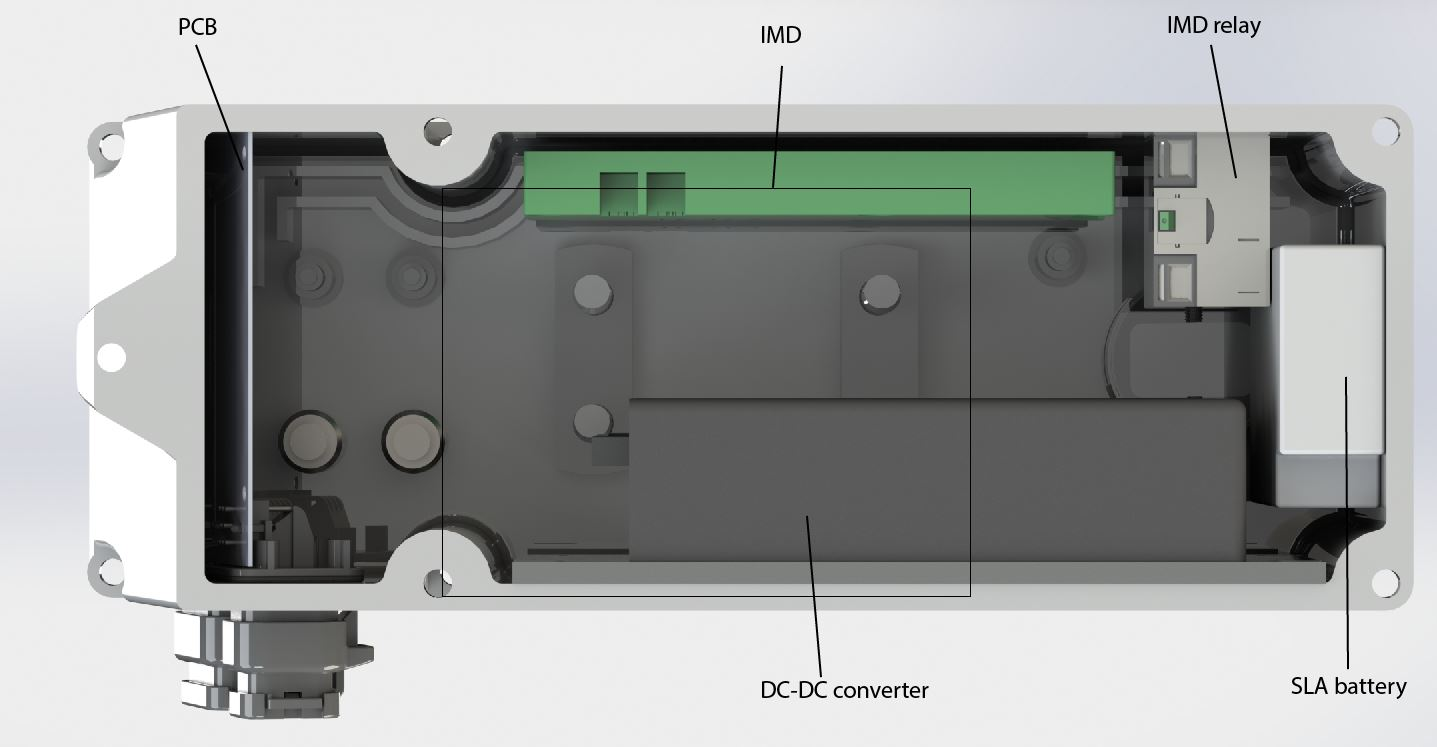
\includegraphics[width = 0.6 \textwidth]{CONTROLPANEL_2}
        \caption{Waterproof Enclosure for most of the shutdown circuit and the TSMPs}
        \label{tsmpbox}
    \end{figure}

    \begin{table}[H]
    \centering
    \begin{tabular}{|l|l|}
    \hline
    TSMP Output Protection Resistor Value & 5 k\ohm \\ \hline
    Resistor Voltage Rating & 122V \\ \hline
    Resistor Power Rating & 3W \\ \hline
    \end{tabular}
    \caption{TSMP Reistor Data}
    \label{tsmptable}
    \end{table}

    \subsection{Pre-Charge System}

    \textit{Describe your design for the pre-charge circuitry. Describe wiring, connectors and cables used.}
    \begin{itemize}
        \item Include a schematic of the pre-charge circuit
        \item Include a plot of calculated TS Voltage vs. time
        \item Include a plot of calculated TS Voltage vs. time
        \item Include a plot of resistor power vs time
    \end{itemize}

    %Include a schematic of the pre-charge circuit

    \begin{figure}[H]
        \centering
        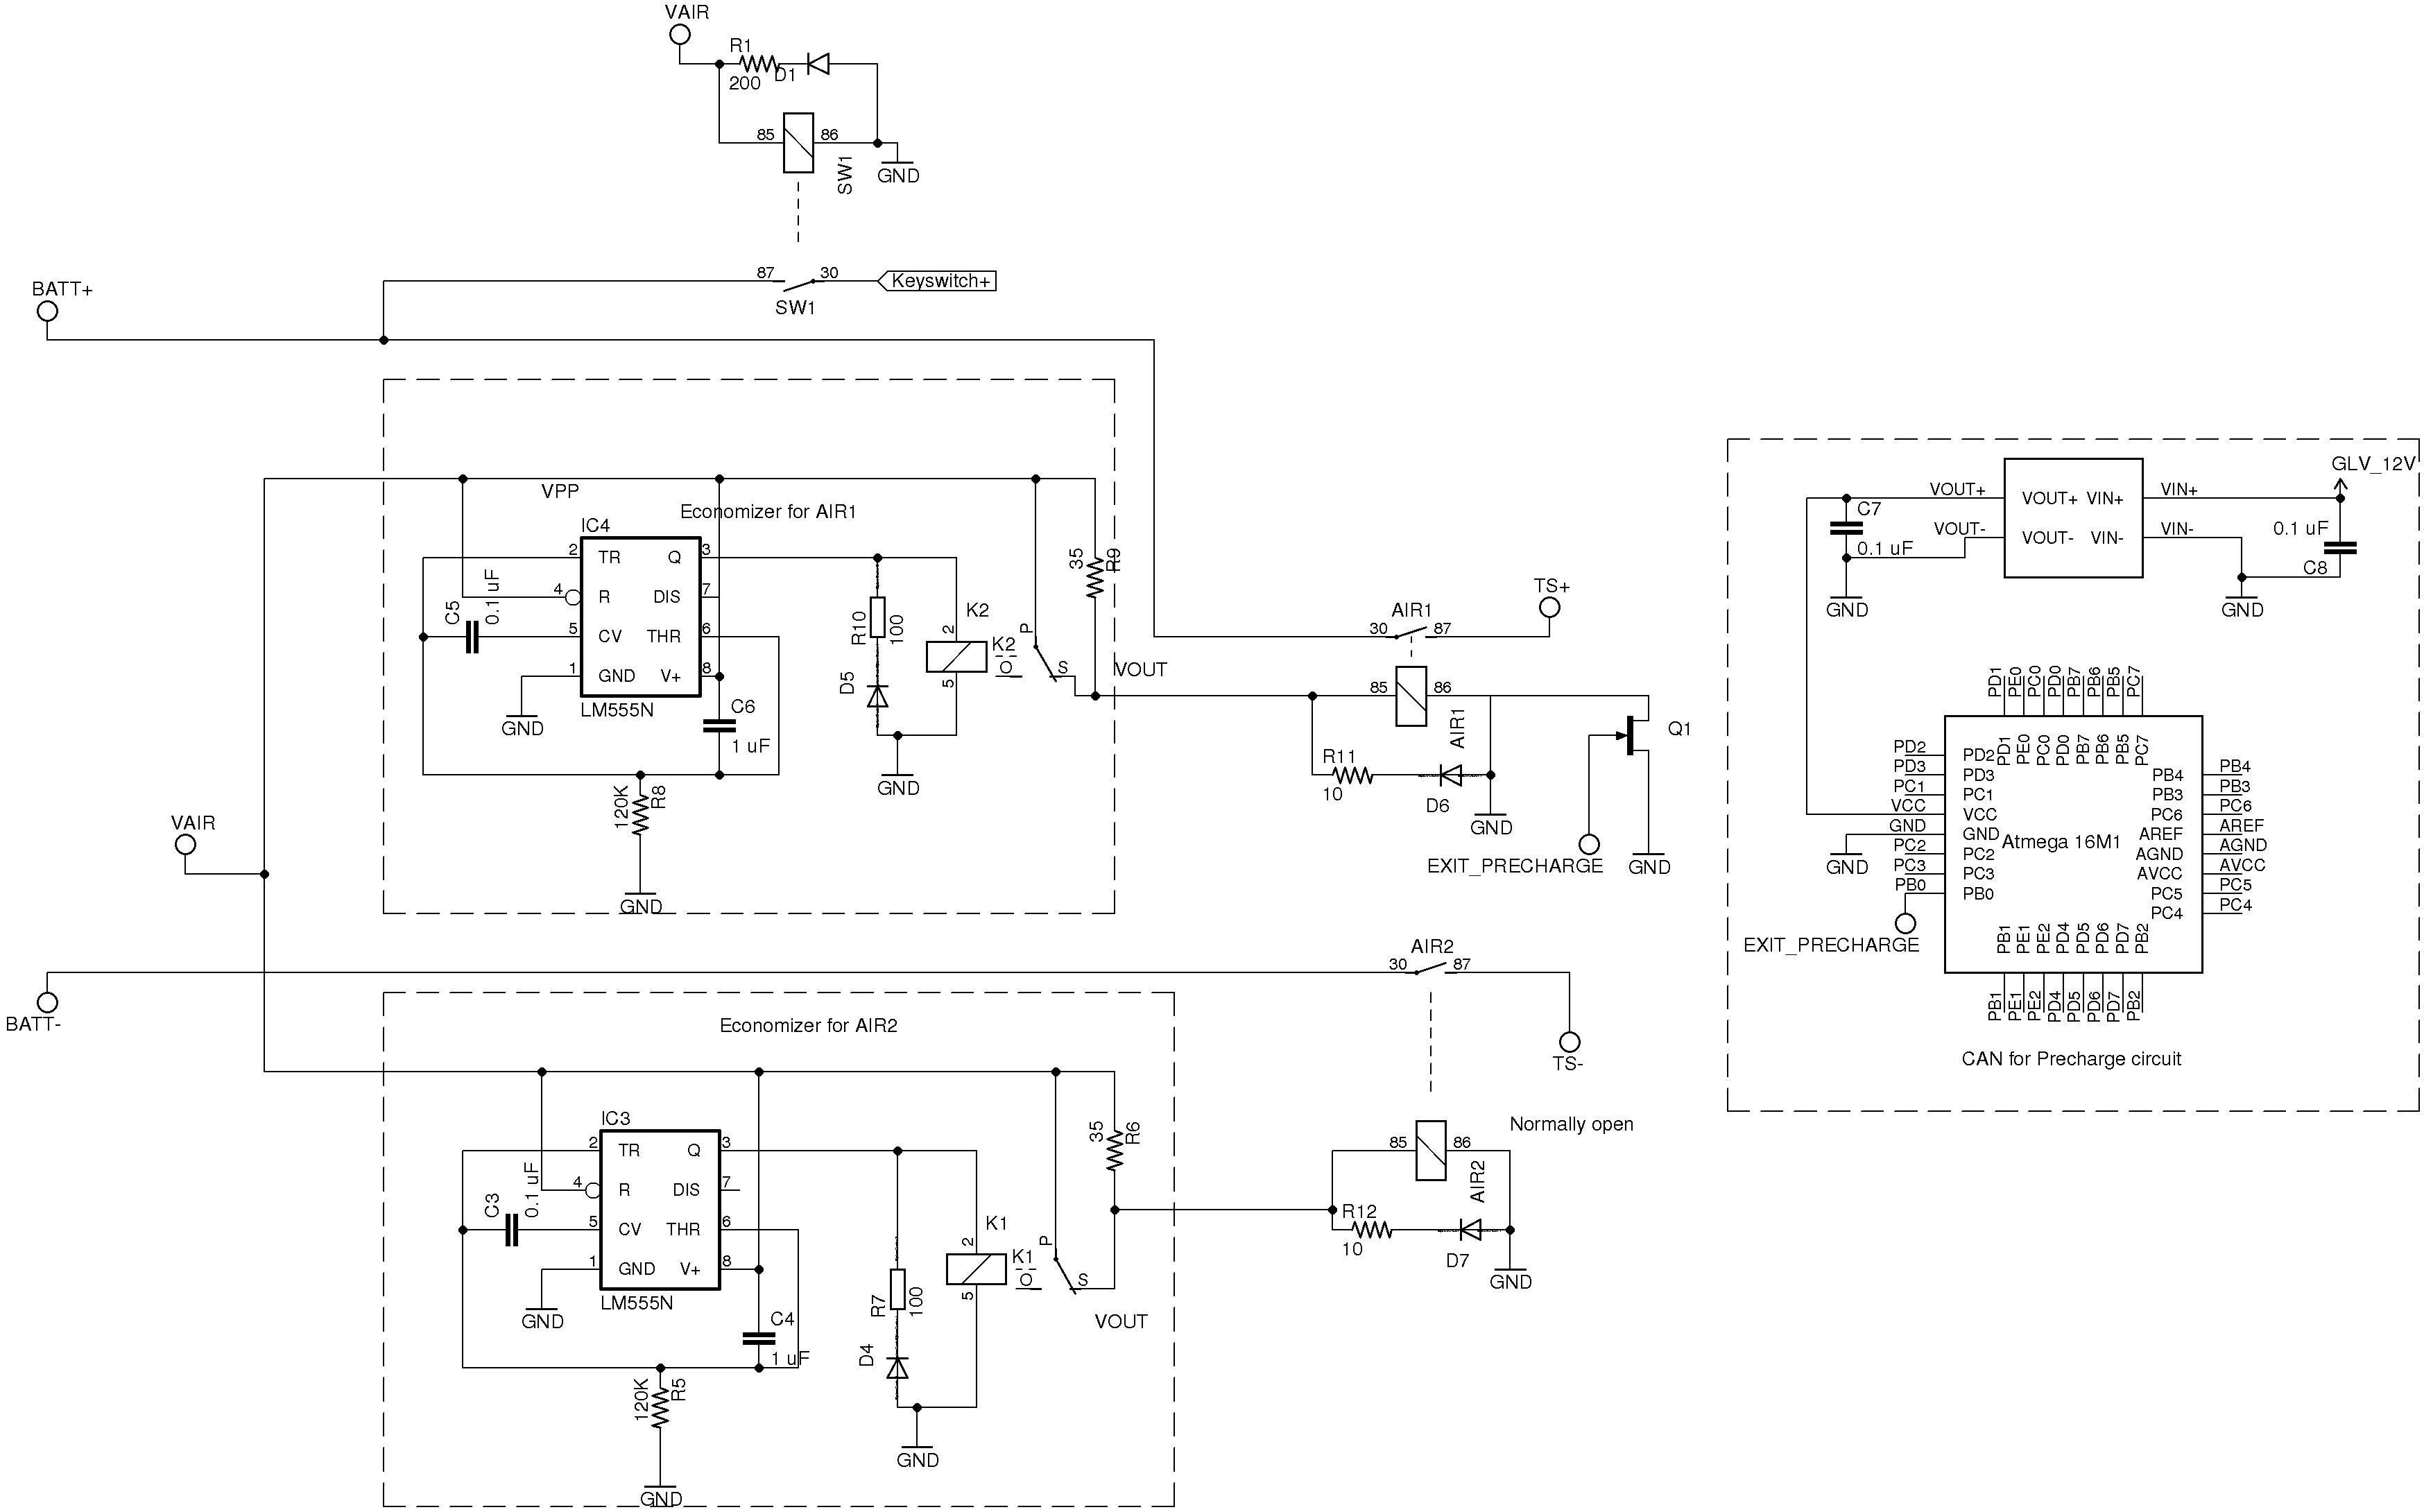
\includegraphics[width = 0.7 \textwidth]{precharge}
        \caption{Precharge System Schematic}
        \label{prechargeschem}
    \end{figure}

    %Describe connectors and cables used
    Ticket \#1209 stated compliance of the internal precharge system of the Sevcon motor controller instead of a separate precharge system consisting of a relay and resistor.

    Once the shutdown circuit is closed, it will immediately power the coils of the normally closed discharge relay, the normally open precharge relay, and the normally open TS- AIR. This opens the discharge relay, and closes the precharge relay and TS- AIR. Instead of connecting Batt+ to TS+ through a current limiting resistor, the precharge relay connects B+ to the key switch terminal on each of the Sevcon motor controllers. When powered by their key switch terminals, the motor controllers charge their internal capacitors up to around 50V for 0.5 seconds, then up to 90V (or another specified voltage) for 0.1 seconds before signaling though the CAN system that the precharge is complete. This CAN message causes a node in the battery to allow the shutdown circuit to close the TS+ AIR.

    In figure \ref{prechargemeasurements}, the voltage of a test setup of the pre-charge system internal to the motor controller was measured. Because there is no resistor other than the motor controller, the current and power could not be calculated and/or graphed. As discussed above, the function describing the pre-charge is stepwise.

        \begin{figure}[H]
        \centering
        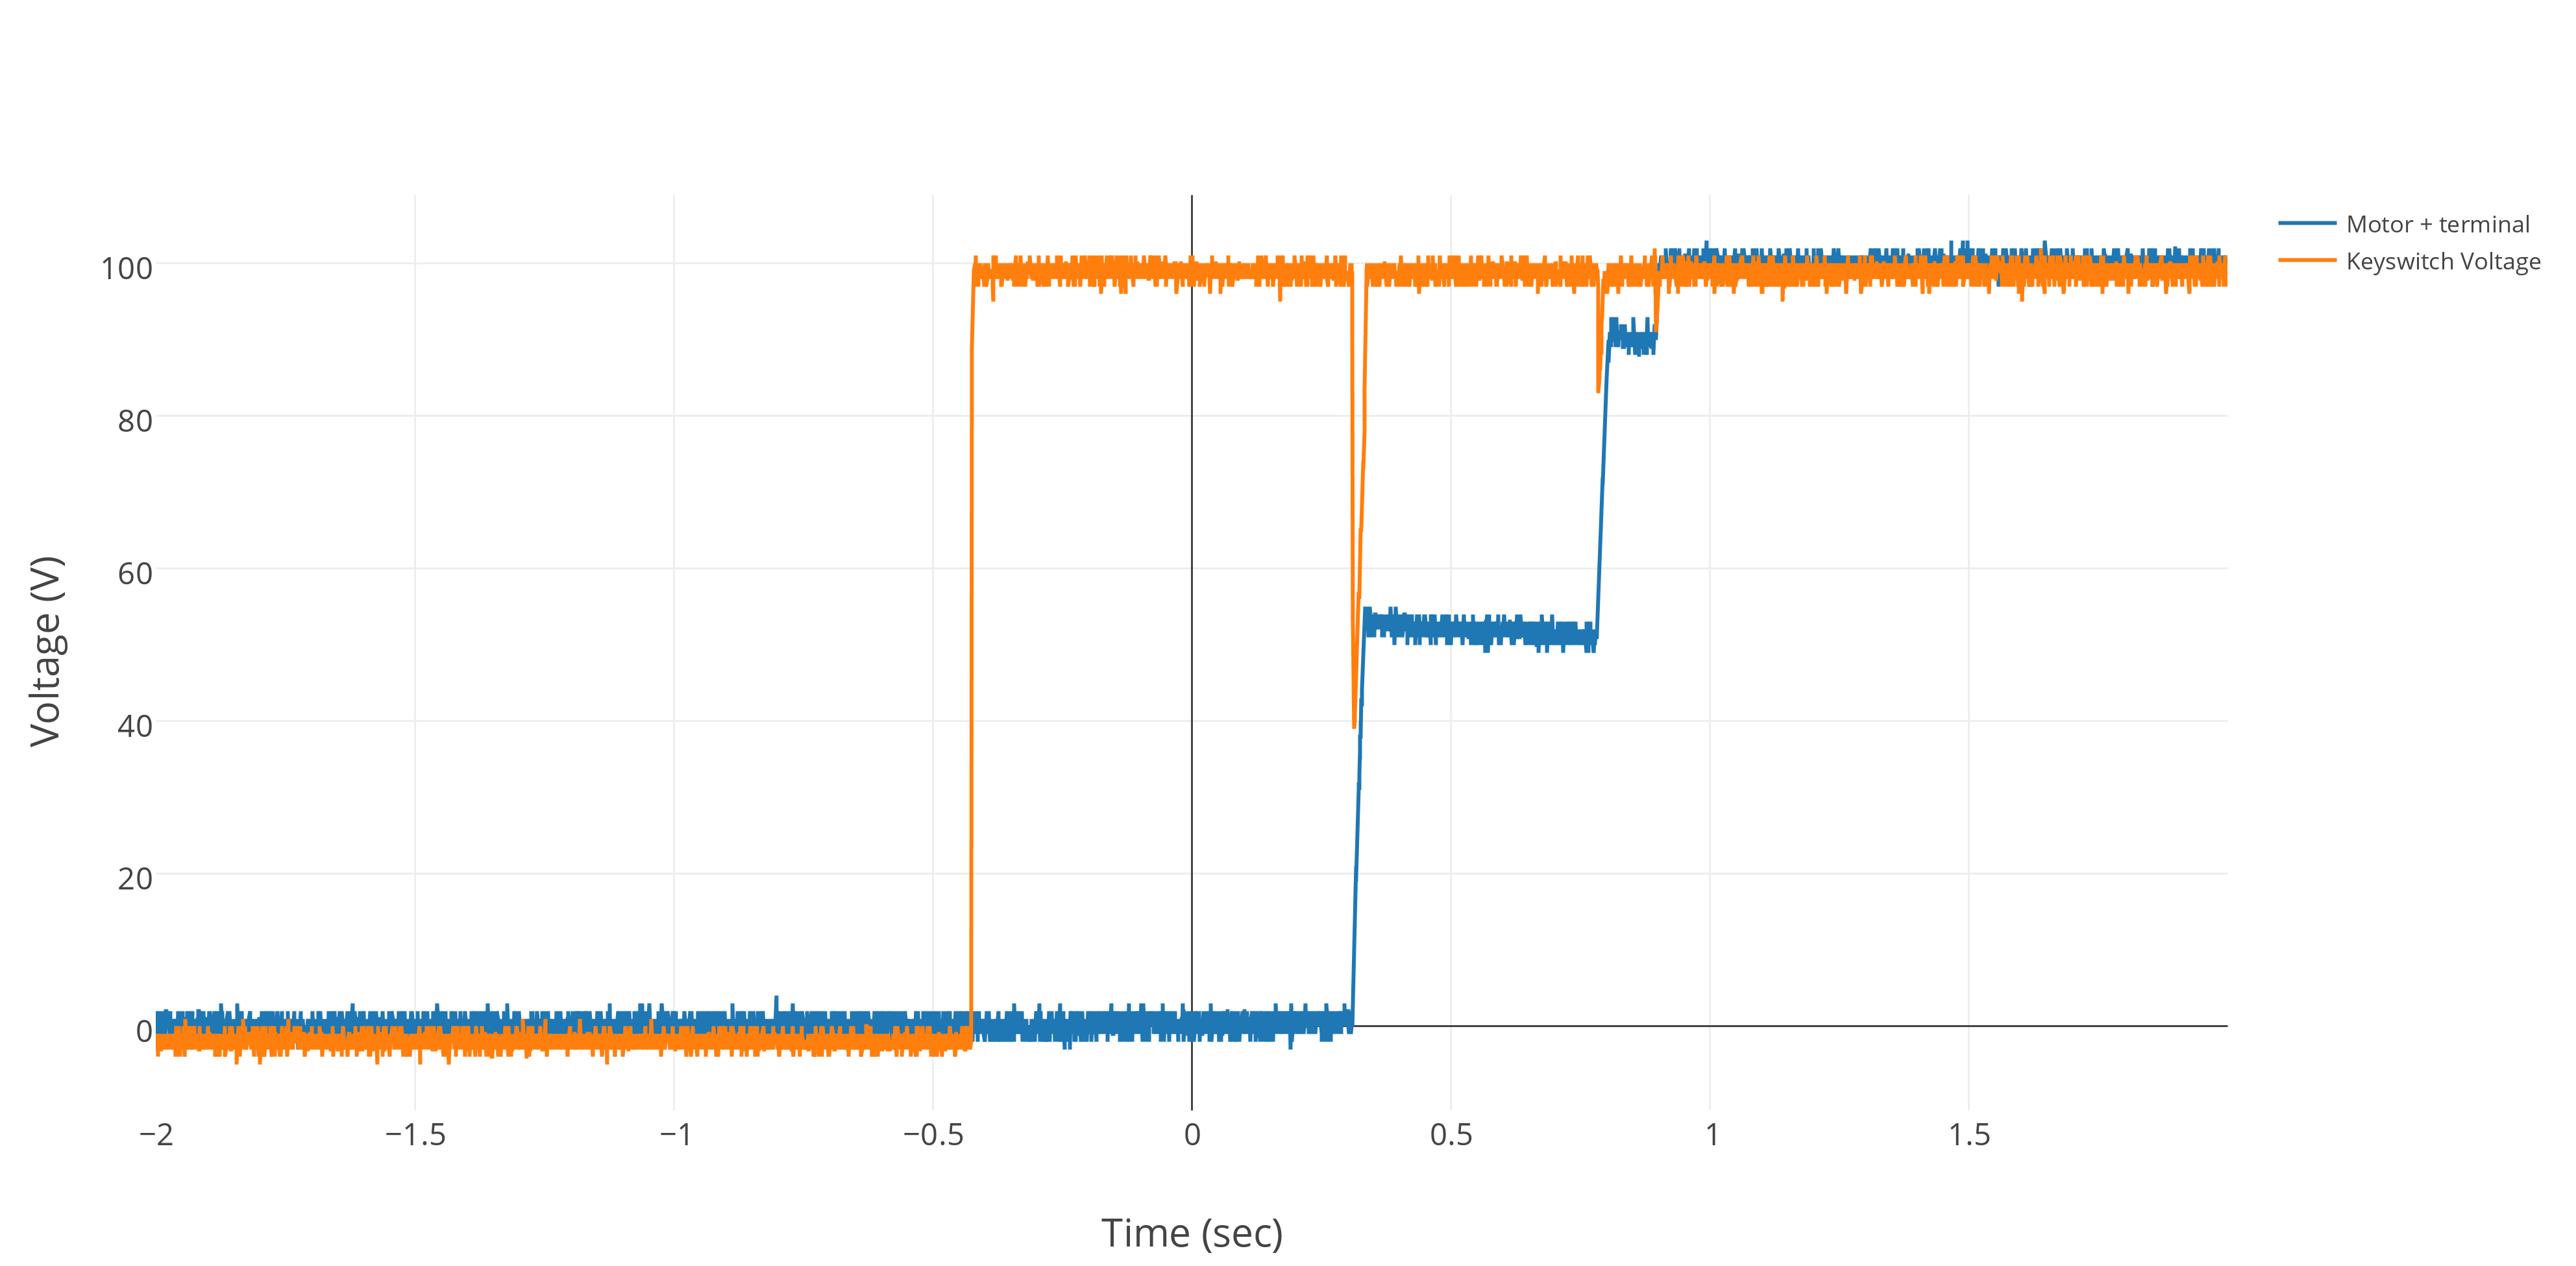
\includegraphics[width = 0.8 \textwidth]{PrechargeVoltage}
        \caption{Measured Precharge voltage for both the motor and the keyswitch activation}
        \label{prechargemeasurements}
    \end{figure}

    \textit{Provide the following information:}

    Because of our use of the motor controller's internal precharge functionality, the vehicle has no separate pre-charge resistor.

    \begin{table}[H]
    \centering
    \begin{tabular}{|l|l|}
    \hline
    Resistor type & N/A \\ \hline
    Resistance & N/A \ohm \\ \hline
    Continuous power rating & N/A W \\ \hline
    Overload power rating & N/A W for\_ sec \\ \hline
    Voltage rating & N/A V \\ \hline
    \end{tabular}
    \caption{Data for the pre-charge resistor}
    \label{prechargerestable}
    \end{table}

    %table of Data for the pre-charge relay

    \begin{table}[H]
    \centering
    \begin{tabular}{|l|l|}
    \hline
    Relay MFR \& Type: & Omron Electronics \\ \hline
    Contact Arrangement & SPST-NO \\ \hline
    Continuous DC contact current & 10A \\ \hline
    Contact voltage rating & 125VDC \\ \hline
    \end{tabular}
    \caption{Data of the pre-charge relay}
    \label{prechargerelaytable}
    \end{table}

    \subsection{Discharge System}

    %Include a schematic of the discharge circuit
    %Replace matlab figures with larger fonts...

    \textit{Describe your concept for the discharge circuitry. Describe wiring, connectors and cables used.}

    \begin{itemize}
        \item Include a schematic of the pre-charge circuit
        \item Include a plot of calculated TS Voltage vs. time
        \item Include a plot of calculated “Discharge current” vs. time
        \item Include a plot of resistor power vs time.
    \end{itemize}

\textit{Provide the following information:}

\begin{figure}[H]
    \centering
    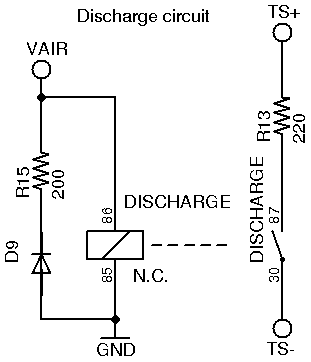
\includegraphics[width = 0.3 \textwidth]{discharge}
    \caption{Schematic of the discharge system}
    \label{dischargeschem}
\end{figure}

    \begin{figure}[H]
        \centering
        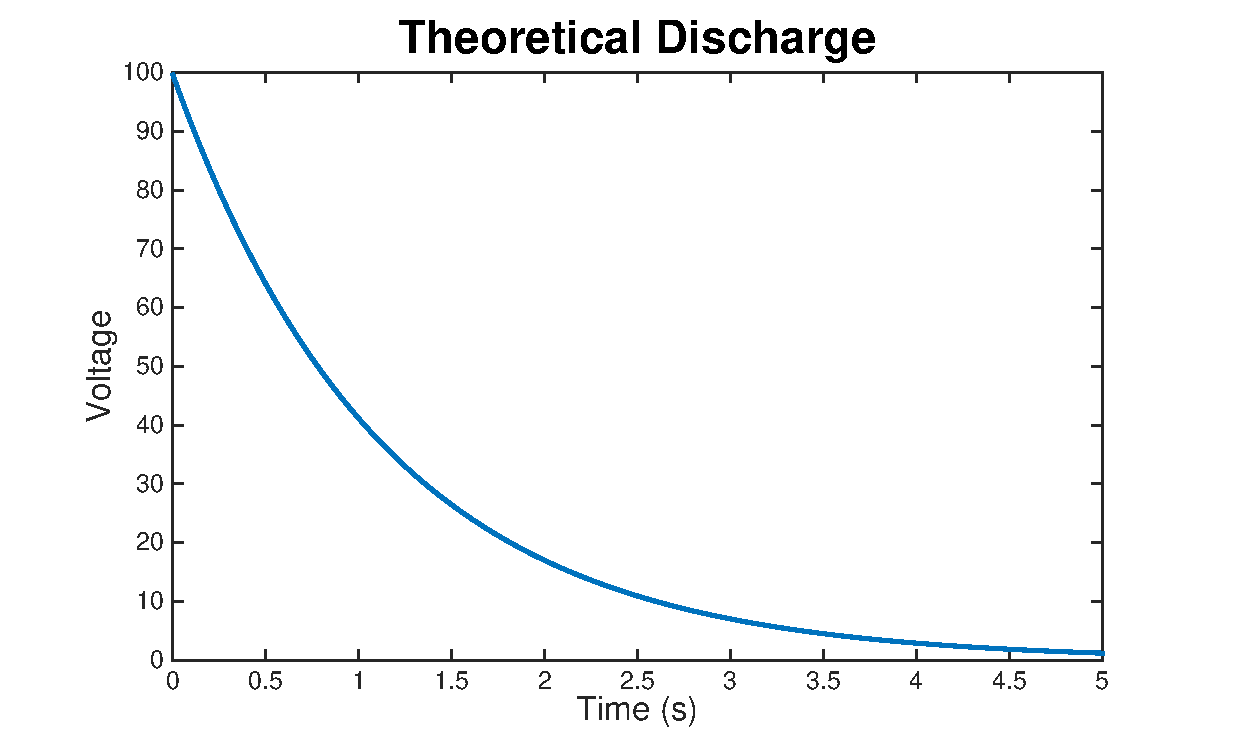
\includegraphics[width = 0.8 \textwidth]{dischargevoltage}
        \caption{Calculated discharge voltage vs. time}
        \label{voltagedischarge}
    \end{figure}

    \begin{figure}[H]
        \centering
        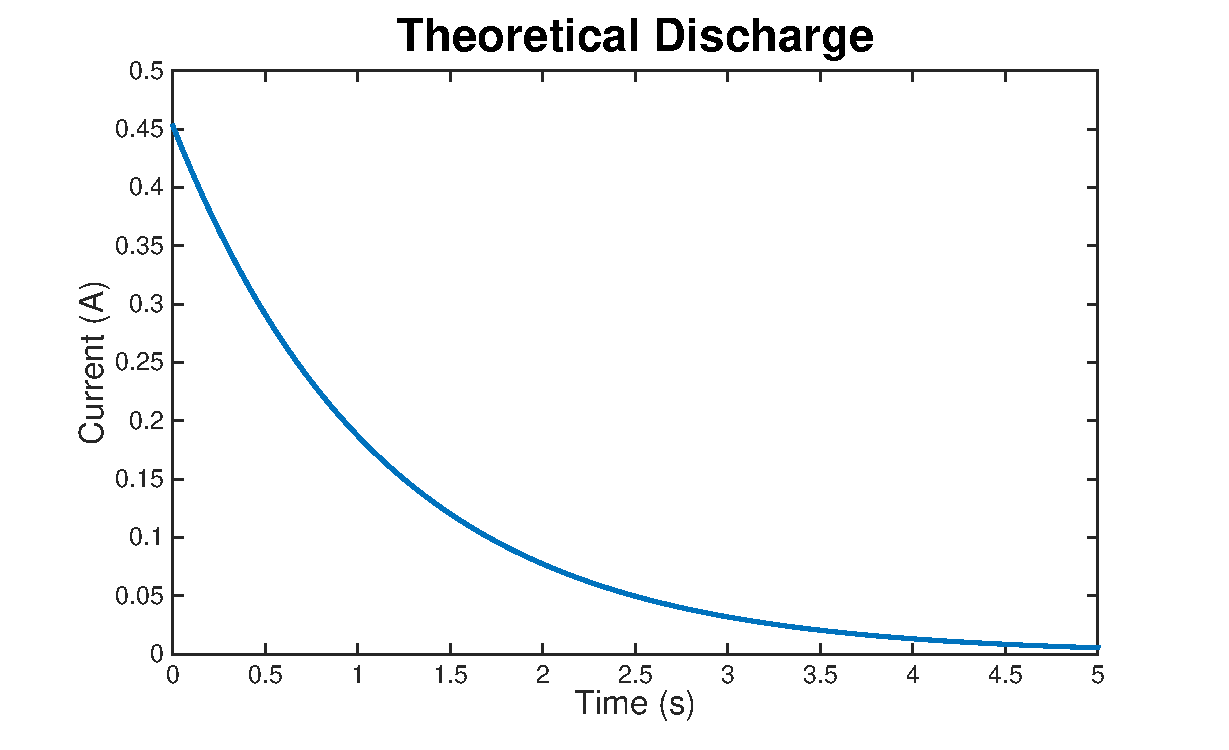
\includegraphics[width = 0.8 \textwidth]{dischargecurrent}
        \caption{Calculated discharge current vs. time}
        \label{currentdischarge}
    \end{figure}

    \begin{figure}[H]
        \centering
        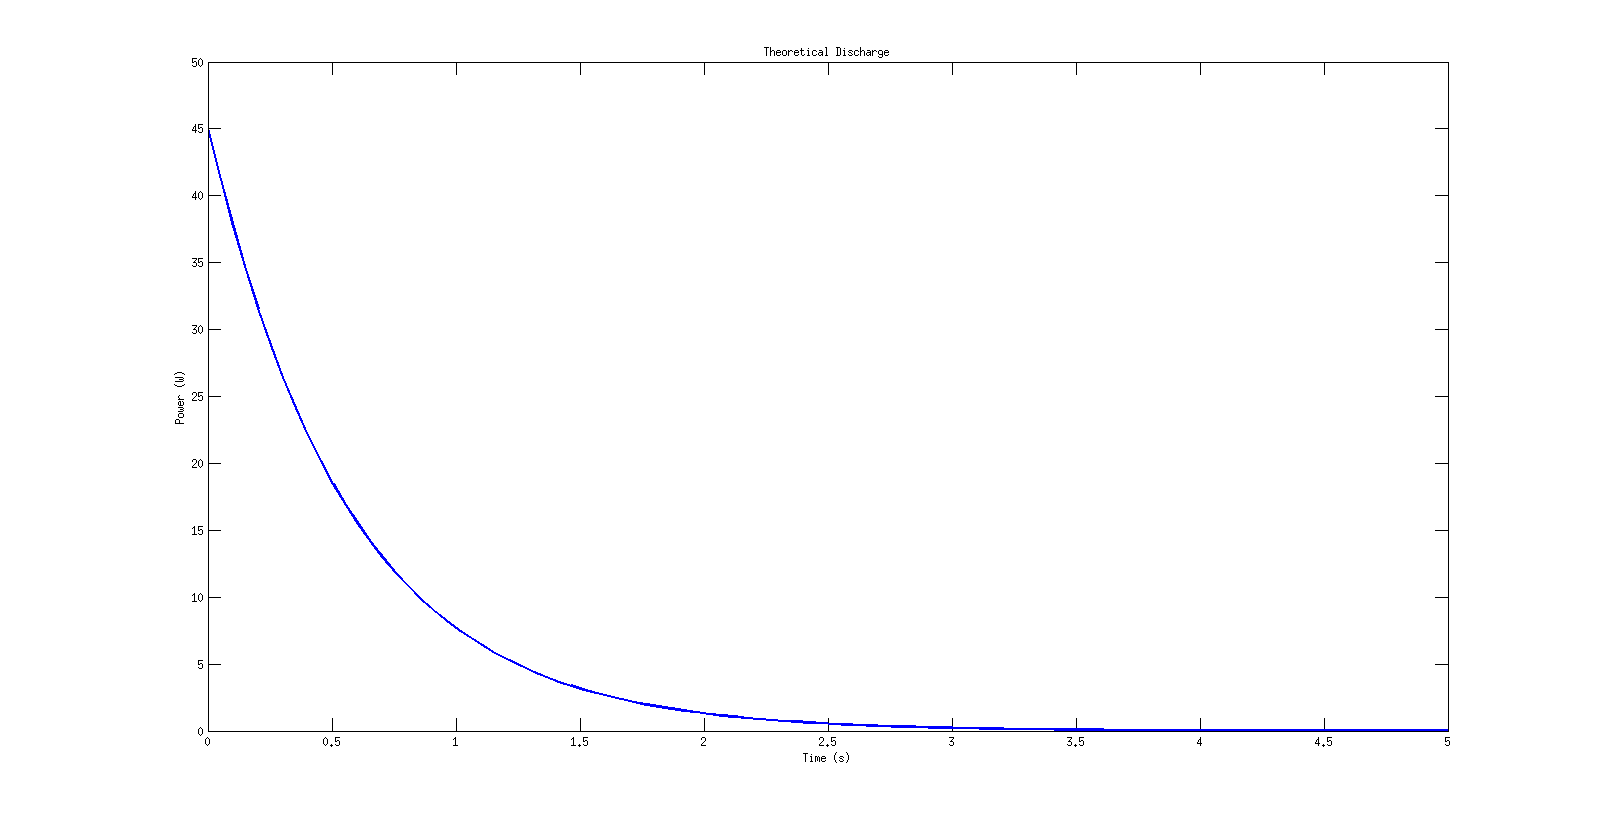
\includegraphics[width = 0.8 \textwidth]{powerdischarge}
        \caption{Calculated discharge power vs. time}
        \label{powerdischarge}
    \end{figure}

    %Table of Data of the discharge circuit.
    \begin{table}[H]
    \centering
    \begin{tabular}{|l|l|}
    \hline
    Resistor Type & \begin{tabular}[c]{@{}l@{}}Aluminium Housed Wirewound \\ Resistor\end{tabular} \\ \hline
    Resistance & 220 \ohm \\ \hline
    Continuous power rating & 50 W \\ \hline
    Overload power rating & Unknown \\ \hline
    Voltage rating & Only power rating listed \\ \hline
    Maximum expected current & 0.45 A \\ \hline
    Average current & 0.1 A \\ \hline
    \end{tabular}
    \caption{Data of the discharge circuit}
    \label{dischargetable}
    \end{table}

    The maximum discharge current and power is calculated as follows:

    \begin{align}
        V = I* R\\
        100 V = I * 220 \ohm \\
        I = 0.45 A \\
        P = I * V\\
        P = 0.45 * 100 \\
        P = 45 W
    \end{align}

    Therefore the 50W, 220\ohm  resistor will be able to handle the power of the discharge circuit continuously, but will only need to handle it for the start of discharge, which itself only lasts 5 seconds.

    \subsection{High Voltage Disconnect (HVD)}

    \textit{Describe your design for the HVD and how it is operated, wiring, and location. Describe how your design meets all requirements for EV4.7}

    \begin{figure}[H]
        \centering
        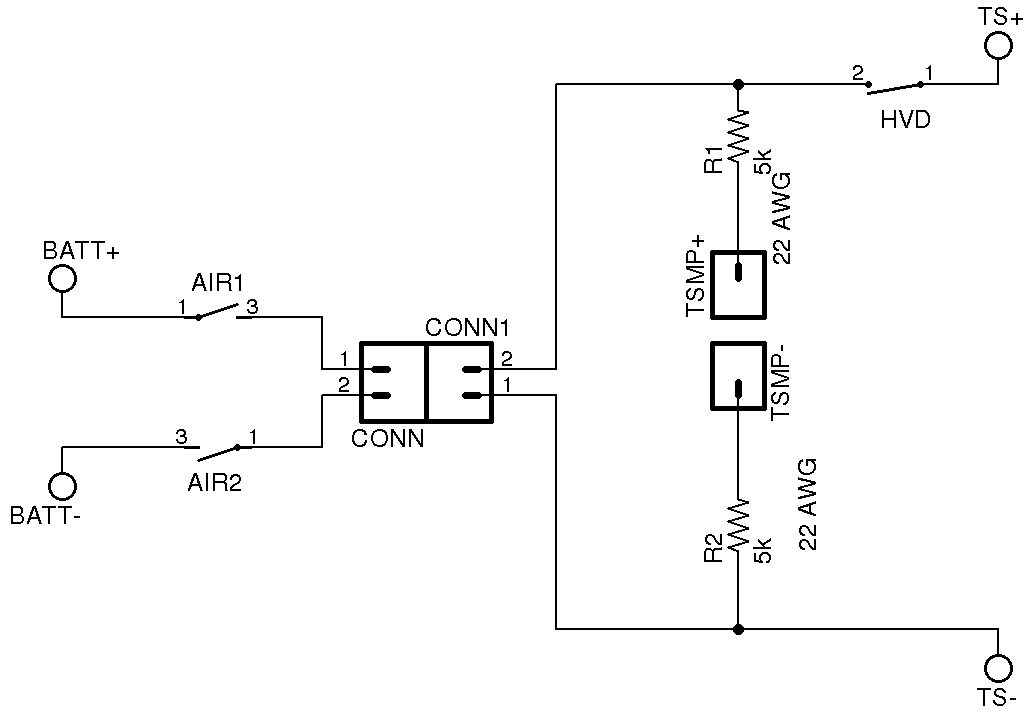
\includegraphics[width = 0.5 \textwidth]{HVD}
        \caption{Electrical connections of the HVD}
        \label{hvdschem}
    \end{figure}

    We will be using an Anderson Power Products SB Smart VEH-G12 HVD (P/N 115158G12 Vehicle Side andP/N 115158G11 Outboard Side) as our high voltage disconnect, provided by Zero Motorcycles.  The part we have in-hand also has a rubber grip on the outboard side of the HVD, which gives the user a better purchase on the HVD, as shown in Figure \ref{hvdpic}.

    \begin{figure}[H]
        \centering
        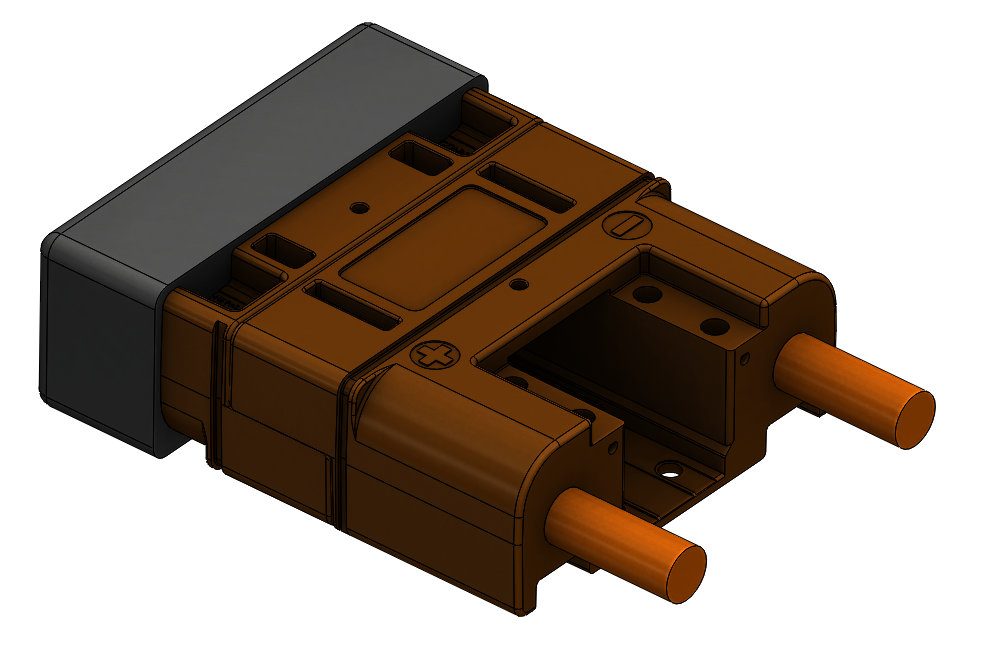
\includegraphics[width = 0.4 \textwidth]{anderson_hvd_interlock}
        \caption{Anderson Power Products SB Smart VEH-G12 HVD}
        \label{hvdpic}
    \end{figure}

    \subsection{Accelerator Actuator / Throttle Position Sensor}

    \textit{Describe the accelerator actuator and throttle position sensor(s) used, describe additional circuitry used to check or condition the signal going to the motor controller. Describe wiring, cables and connectors used. Provide schematics and a description of the method of operation of any team-built signal conditioning electronics. Explain how your design meets all of the requirements of FH Rules IC1.6 and EV2}

    %Throttle Position encoder data

    \begin{table}[H]
    \centering
    \begin{tabular}{|l|l|}
    \hline
    Actuator/Encoder MFR and model & Magni-Tec MHR5621 \\ \hline
    Encoder principle & \begin{tabular}[c]{@{}l@{}} Dual-Rotary \\ Potentiometer\end{tabular} \\ \hline
    Output & Analog \\ \hline
    \begin{tabular}[c]{@{}l@{}}Is motor controller \\ accelerator signal isolated \\ from TSV?\end{tabular} & No \\ \hline
    \begin{tabular}[c]{@{}l@{}}If no, how will you satisfy rule \\ EV2.3?\end{tabular} & Isolated tranceiver on CAN \\ \hline
    \end{tabular}
    \caption{Throttle Position Encoder Data}
    \label{throttletable}
    \end{table}

    The 2 throttle encoder outputs (2 electrically-separated potentiometers contained within MHR5621) will be sensed through a CAN node input pin. The CAN node will then log the information (no amplification in any way) and send it to the motor controller CAN node. That CAN node will output the same analog signal through an optoisolator to separate it from the GLV system and ground it to the TS system.

    \textnormal{There will be two electrically-separated potentiometers being sensed by a CAN node. There will be pull-down resistors on both inputs in order to detect wire-failure for the potentiometer's input. Software will detect whether the potentiometer inputs are within 10\% of each other, as well as checking that the potentiometer readings are within the limits of the system.}\\

    \textnormal{Once the throttle has been read and sanitized by the CAN node, it will be sent along the CAN line to the motor controller CAN node. This node can send isolated analog signals to both motor-controllers for torque control. This node will also take into account the steering-wheel sensor and may decrease the torque signal to one of the motors in order to allow for a virtual differential. It will never increase the torque signal.}\\

    \textnormal{This design meets all rules requirements because the system is galvanically isolated from the motor controller inputs and our system is able to detect all the plausible failure modes of the potentiometer.}


    \subsection{Accelerator / Throttle Position Encoder Error Check}

    \textit{Describe how the system reacts if an error (e.g. short circuit or open circuit or equivalent) is detected. Describe circuitry used to check or condition the signal going to the motor controller. Describe how failures (e.g. Implausibility, short circuit, open circuit etc.) are detected and how the system reacts if an error is detected. State how you comply with EV2.2}


    \textnormal{
    There are two main errors that need to be considered. Potentiometer input failure, as in a wire being disconnected or an invalid signal, and CAN system failure, as in invalid message objects are sent.
    }\\

    \textnormal{
    In the case of a short or open-circuit for potentiometer input failure, there will be a pull-down resistor which will pull the value read at the input pin to 0V (and in case of a short it will be pulled to 5V). Any reading not in the range of 1V-4V will be considered an error and will be dealt with in software. No throttle command will be sent in this case.
    }\\

    \textnormal{
    In the case of CAN message failure, the CAN node which is connected to the motor-controllers will not send any throttle command if no valid throttle message is read every 0.1 seconds.
    }

\section{Accumulator System}

        Person primarily responsible for this section:

            \begin{table}[H]
                \centering
                \label{responsible5}
                \begin{tabular}{lr}
                Name: & Lisa Hachmann \\ \hline
                e-mail: & Lisa.Hachmann@students.olin.edu \\ \hline
                \end{tabular}
            \end{table}

    \subsection{Accumulator Pack}

        \textit{Provide a narrative design of the accumulator system and complete the following table.}

        All cell information listed was recorded from actual measurements. Manufacturer data is under NDA and restricted until we receive permission to release this information to the Formula Hybrid team.

            \begin{table}[H]
                \centering
                \begin{tabular}{|l|l|}
                \hline
                Maximum Voltage (during charging) & NDA \\ \hline
                Nominal Voltage & 3.75 VDC (7.5VDC per module) \\ \hline
                Total number of cells & 48 \\ \hline
                Cell arrangement & \begin{tabular}[c]{@{}l@{}}2s2p in one module,\\ 12 modules in series\end{tabular} \\ \hline
                Are packs commercial or team constructed & Team \\ \hline
                Total Capacity (per FH Rules Appendix A) & Less than 5.4 kWh, NDA \\ \hline
                Maximum Segment Capacity & Less than 6 MJ, NDA \\ \hline
                Number of Accumulator Segments & 4 \\ \hline
                \end{tabular}
                \caption{Main accumulator parameters}
                \label{mainaccumtable}
            \end{table}

        \textit{Describe how pack capacity is calculated. Provide calculation at 2C (0.5 hour) rate? How is capacity derived from manufacturer’s data? If so, include discharge data or graph here. Include Peukert calculation if used (See FH Rules Appendix A). Show your segment energy calculations.}

        The segment energy is calculated as: Vnom x Cell AH (2C rate) x Number of Cells x 3.6 kJ (The 80\% factor is not applied for this calculation). Each segment is 1/4 of the total accumulator (3 modules). Module/Cell current at 2C discharge is under NDA, but is included in the cell manufacturer's datasheet.

            % \begin{align}
            %     \text{Seg Energy} &= V_{nom} * \text{Cell Ah (2C rate)} * \text{Number of Cells} *  %     3.6 \text{kJ}\\
            %     \text{Seg Energy} &= 7.5 * 65 * 3* 3.6 \\
            %     \text{Seg Energy} &= 5265 \text{kJ}\\
            %     \text{Seg Energy} &= 5.265 \text{MJ}
            % \end{align}

    \subsection{Cell Description}

        \textit{Describe the cell type used and the chemistry and complete the following table.}

        The cells used are Automotive Energy E5 lithium ion (pouch type) cells, and they were fabricated into modules by Nissan for their Nissan Leaf electric vehicle. Their datasheets are not included because of our team's NDA with Nissan. We are working to be able to share the necessary information, but the cell values are from our testing of the cells.
        %ticket number of approval

            \begin{table}[H]
                \centering
                \begin{adjustbox}{max width=\textwidth}
                \begin{tabular}{|l|l|}
                \hline
                Cell Manufacturer and Model & \begin{tabular}[c]{@{}l@{}}Automotive Energy Supply Corporation\\ Model E5\end{tabular} \\ \hline
                Cell type & Pouch type, Yes \\ \hline
                Are these pouch cells & Yes \\ \hline
                Cell nominal capacity at 2C (0.5 hour) rate & NDA \\ \hline
                Datasheet nominal capacity & NDA\\ \hline
                Maximum Voltage (during charging) & NDA \\ \hline
                Nominal Voltage (data sheet value) & 3.75 V (not datasheet value) \\ \hline
                Minimum Voltage (AMS setting) & NDA \\ \hline
                Maximum Cell Temperature (charging - AMS setting) & NDA  \\ \hline
                Maximum Cell Temperature (discharging - AMS setting) & NDA \\ \hline
                Cell Chemistry & \begin{tabular}[c]{@{}l@{}}Lithium Ion - Laminate type\\ Cathode/Anode Material: LiMn2O4 with LiNiO2/Graphite\end{tabular} \\ \hline
                \end{tabular}
                \end{adjustbox}
                \caption{Main cell specification}
                \label{cellspectable}
            \end{table}

        \textit{Show your calculations for 2C nominal AH capacity if the data sheet uses a different discharge rate. Refer to FH rules Appendix A}

        Calculations at 2C nominal Ah capacity were used to confirm compliance with FH rules, but cannot be shared at this time.

    \subsection{Cell Configuration}

            \begin{figure}[H]
                \centering
                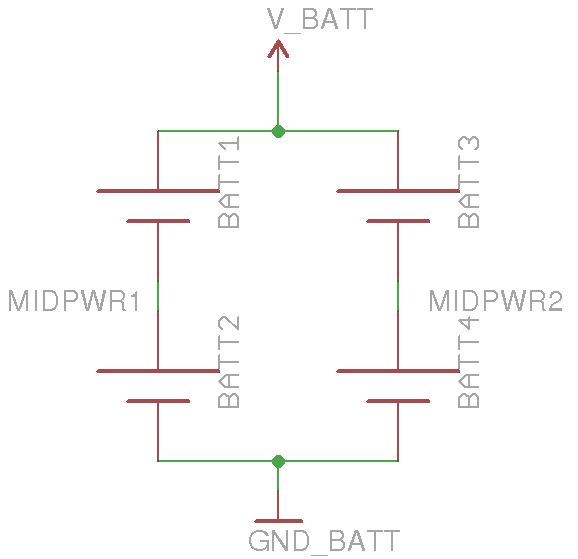
\includegraphics{moduleschem}
                \caption{Schematic of one module, which includes 4 cells in a 2s-2p configuration, with shutdown separators in the middle of the parallel strings of cells}
                \label{moduleschem}
            \end{figure}

        \textit{Describe cell configuration, show schematics, cover additional parts like internal cell fuses etc. Describe configuration: e.g., N cells in parallel then M packs in series, or N cells in series then M strings in series.}

        The full accumulator has 12 modules in series. Each module has 2 cells in series in 2 parallel strings, shown in Figure \ref{moduleschem}. Therefore, the full configuration is 12s(2s2p).

        \textit{Does the accumulator combine individual cells in parallel without cell fuses? \makebox[0pt][l]{$\square$}\raisebox{.15ex}{\hspace{0.1em}$\checkmark$} \hspace{0.2cm} Yes
        \makebox[0pt][l]{$\square$}\raisebox{.15ex}{\hspace{0.1em}} \hspace{0.2cm} No}

        The modules (which are all in series), each have a string of cells in parallel, as seen in Figure \ref{moduleschem}. However, in the middle of the string of cells there is a shutdown separator. The shutdown separator between the parallel cells acts as a fuse in over-current conditions. The terminal marked in white in Figure \ref{canopener} references the point between the two parallel cell strings. These modules are commercially sold in Nissan Leaf vehicles without issue, so we are referencing their safety to prove ours.
        %Need to include their certification in ESF.

    \subsection{Segment Maintenance Disconnect}

        %table of SMD data
        \textit{Describe segment maintenance disconnect (SMD) device, locations, ratings etc.}

            \begin{table}[H]
                \centering
                \begin{tabular}{|l|l|}
                \hline
                Is HVD used as SMD? & No \\ \hline
                Number of SMD devices & 3 \\ \hline
                SMD MFR and Model & \begin{tabular}[c]{@{}l@{}}SMD - Lear Corporation\\ Fuse inside: Bussman EV30-350\end{tabular} \\ \hline
                SMD Rated Voltage (if applicable) & 500V \\ \hline
                SMD Rated Current (if applicable) & 350A \\ \hline
                Segment Energy (6 MJ max) & 4.86 MJ \\ \hline
                \begin{tabular}[c]{@{}l@{}}Segment Energy Discharge Rate\\ (Ref FH Rules Appendix A)\end{tabular} & \textcolor{red}{2C} \\ \hline
                \end{tabular}
                \caption{SMD Data}
                \label{smdtable}
            \end{table}

\subsection{Lithium Ion Pouch Cells}

    \textit{The vehicle accumulator uses individual pouch cells. } \par                      \makebox[0pt][l]{$\square$}\raisebox{.15ex}{\hspace{0.1em}} \hspace{0.2cm} Yes
    \makebox[0pt][l]{$\square$}\raisebox{.15ex}{\hspace{0.1em}$\checkmark$} \hspace{0.2cm} No

    \textit{\textcolor{red}{Note that designing an accumulator system utilizing pouch cells is a substantial engineering undertaking which may be avoided by using prismatic or cylindrical cells.} If your team has designed your accumulator system using individual Lithium-Ion pouch cells, include drawings, photographs and calculations demonstrating compliance with all sections of rule EV3.9. If your system has been issued a variance to EV3.9 by the Formula Hybrid rules committee, include the required documentation from the cell manufacturer.}

    Our team has designed an accumulator using modules that include individual lithium-ion pouch cells. However, these modules are unmodified OEM units, used in the Nissan Leaf. We opened ticket \#1084 clarifying our accumulator plans and received permission to include the modules as they are without including a separate method of cell compression.

        \begin{figure}[H]
            \centering
            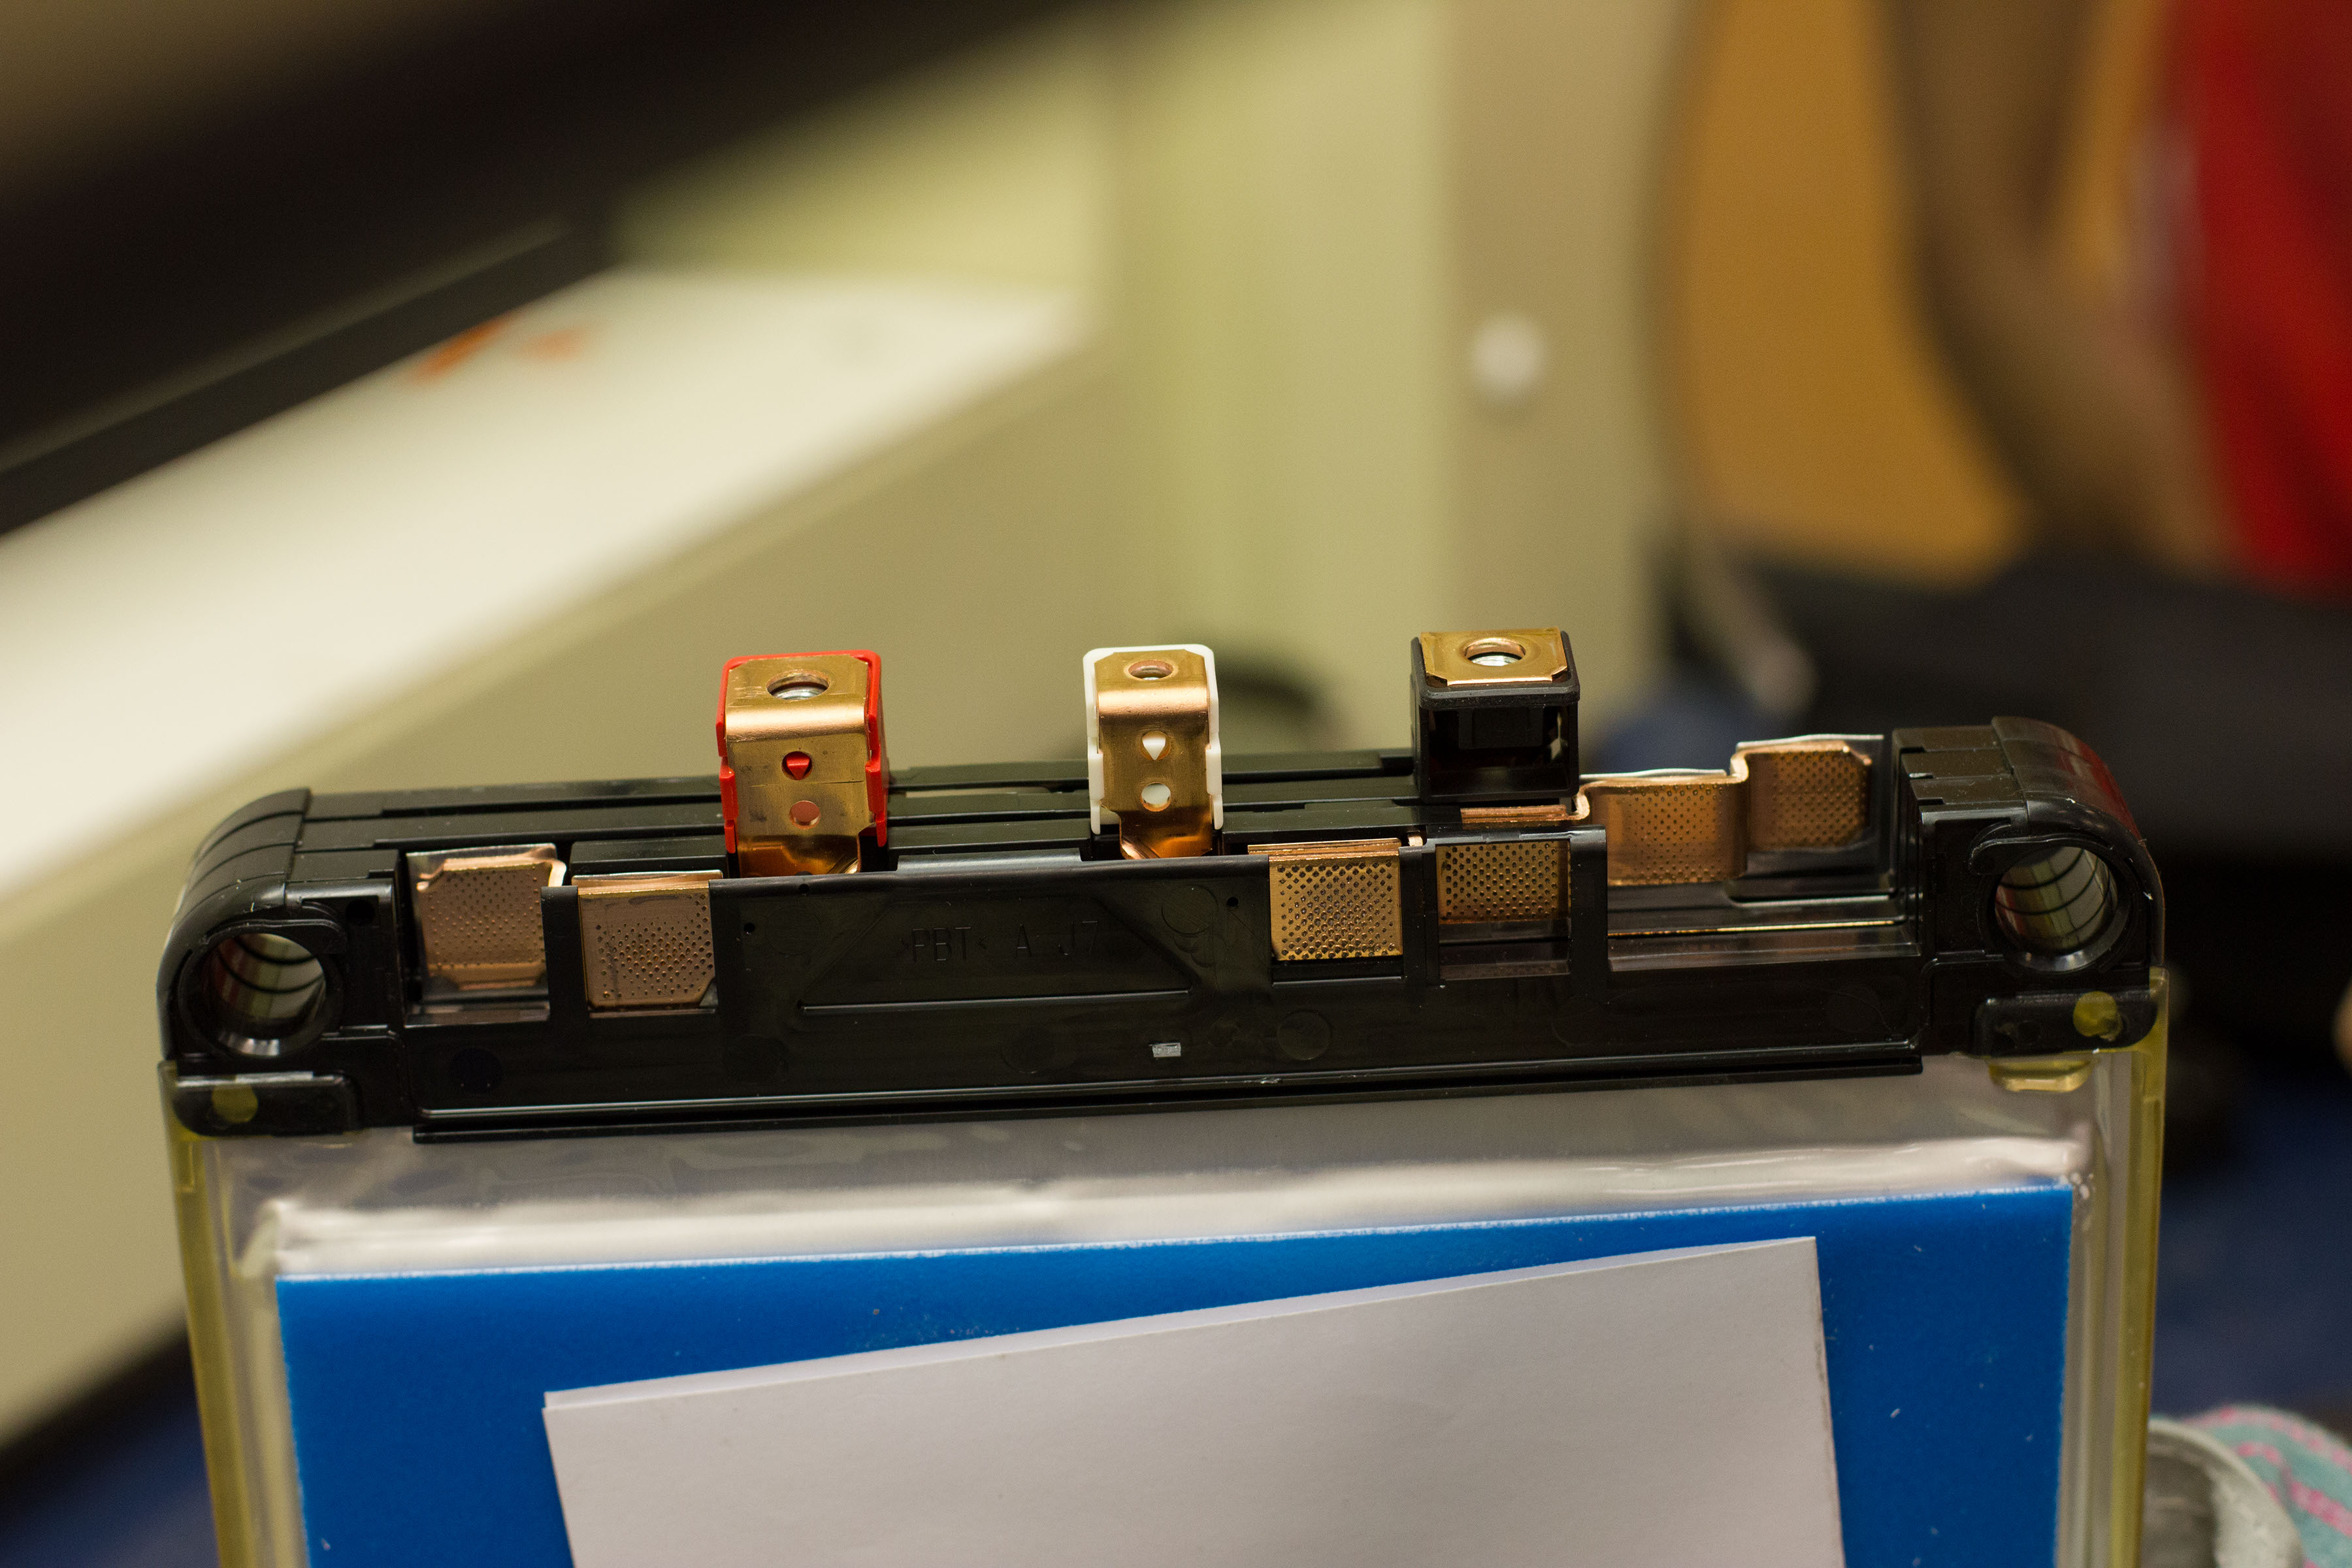
\includegraphics[width = 0.7 \textwidth]{OpenModule}
            \caption{Inside view of a module. }
            \label{canopener}
        \end{figure}


    %If your team has designed your accumulator system using individual Lithium-Ion pouch cells, include drawings, photographs and calculations demonstrating compliance with all sections of rule EV3.9.  If your system has been issued a variance to EV3.9 by the Formula Hybrid rules committee, include the required documentation from the cell manufacturer.

\subsection{Cell Temperature Monitoring} \label{celltopsection}

    \textit{Describe how the temperature of the cells is monitored, where the temperature sensors are placed, how many cells are monitored, etc. Show a map of the physical layout. Provide schematics for team-built electronics.}

    %Show a map of the physical layout. Provide schematics for team-built electronics.

        \begin{figure}[H]
            \centering
            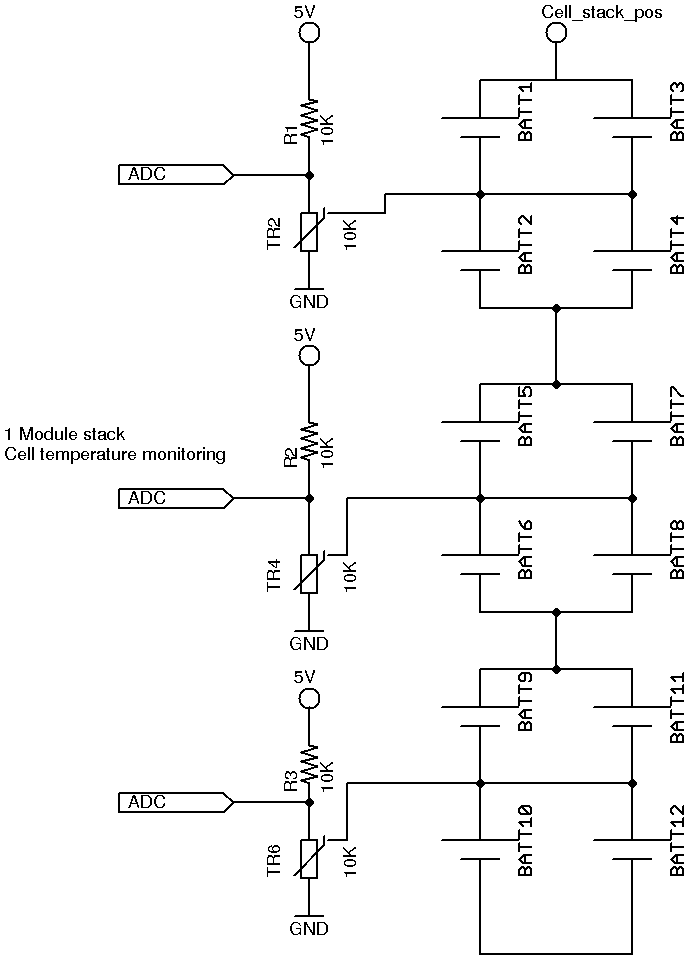
\includegraphics[width = 0.4 \textwidth]{celltemp}
            \caption{Schematic of the temperature monitoring in one segment (3 modules)}
            \label{celltemp}
        \end{figure}


     The temperature of the cells is monitored using 10K thermistors attached to the negative terminals. The middle pole of each module is considered the ground of two cells. Each module's midpoint is measured and one out of three module grounds is measured per accumulator segment. The thermistors are used to form four voltage dividers. When the temperature of the cells increases, the resistance decreases, resulting in less voltage drop across the thermistor. Four analog to digital converters attached to each of the voltage dividers is then used by the Atmega 16M1 used in the CAN system to determine whether the temperature is too high or low. If the temperature is out of range, the shutdown system activates. There is a pull up resistor that pushes the output voltage to 5V if the ADC is a past a certain threshold and 0V otherwise. Because we are monitoring the negative terminals of half of the cells in each module, we are monitoring 50\% of the total cells.

    %table of cell temperature monitoring

        \begin{table}[H]
            \centering
            \begin{tabular}{|l|l|}
            \hline
            Number of Cells with Temperature Monitoring &  24\\ \hline
            Total Number of Cells & 48 \\ \hline
            Percentage Monitored & 50\% \\ \hline
            Percentage Required by FH Rules & 30\% \\ \hline
            If sensor monitors multiple cells, state how many & 2: see Fig. \ref{celltemp} \\ \hline
            \end{tabular}
            \caption{Cell Temperature Monitoring}
            \label{celltempmonitoring}
        \end{table}

\subsection{Accumulator Isolation Relays}

    \textit{Describe the number of AIRs used and their locations. Also complete the following table.}

    The AIRs used are EV Kilovac 200 SPST relays from Tyco Electronics. The relays require the use of an economizer, which switches their current after 150 ms so they do not draw as much current. The economizer circuitry is shown in figure \ref{econschem} for reference. The positive pole AIR and negative pole AIR are located in the accumulator, separated from the cells by two sheets of 1/32" FR4/G10, sandwiching a 0.035" thick 403 stainless steel panel.


        %table of AIR data
        \begin{table}[H]
            \centering
            \begin{tabular}{|l|l|}
            \hline
            MFR \& Model & \begin{tabular}[c]{@{}l@{}}Tyco Electronics, \\ Kilovac EV200\end{tabular} \\ \hline
            Contact arrangement & 1 form x (SPST-NO-DM) \\ \hline
            Continuous DC current rating & 500A \\ \hline
            Overload DC current rating & NEED \\ \hline
            Max operation voltage & 900VDC \\ \hline
            Nominal coil voltage & 9 -36 VDC \\ \hline
            Normal Load switching & See figure \ref{airsdata} \\ \hline
            \end{tabular}
            \caption{AIR data}
            \label{airtable}
        \end{table}


        \begin{figure}[H]
            \centering
            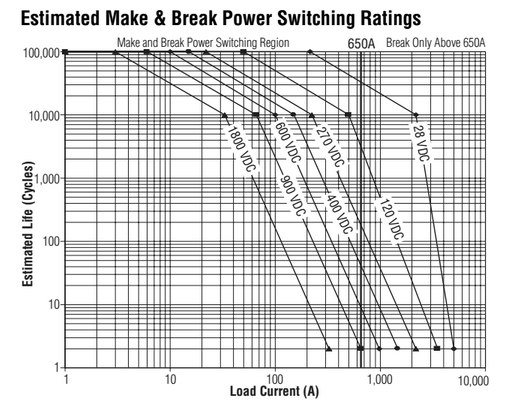
\includegraphics[width = 0.5 \textwidth]{airs}
            \caption{Switching specification for the AIR relay datasheet}
            \label{airsdata}
        \end{figure}

        \begin{figure}[H]
            \centering
            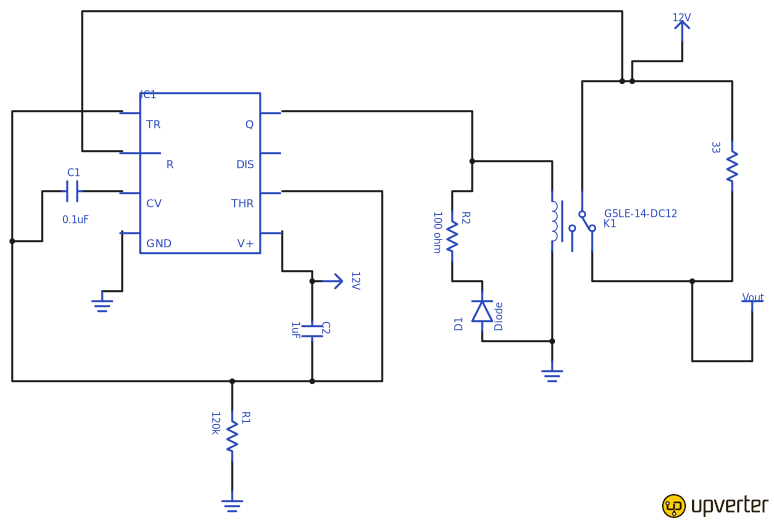
\includegraphics[width = 0.7 \textwidth]{Econcircuit}
            \caption{Circuitry used with the AIRs to enable them to have a lower current draw}
            \label{econschem}
        \end{figure}

\subsection{Accumulator Management System}

    \textit{Describe the AMS and how it was chosen. Describe generally how it meets the requirements of EV3.7}

        %table of AMS data
        \begin{table}[H]
            \centering
            \begin{tabular}{|l|l|}
            \hline
            AMS MFR and Model & Team-made \\ \hline
            Number of AMSs & 4 \\ \hline
            Upper cell voltage trip & NDA \\ \hline
            Lower cell voltage trip & NDA \\ \hline
            Temperature trip & NDA \\ \hline
            \end{tabular}
            \caption{AMS Data}
            \label{amstable}
        \end{table}

        \textit{\begin{itemize}
            \item Describe other relevant AMS operation parameters.
            \item Describe how many cells are monitored by each AMS board, the configuration of the cells, the configuration of the boards and how AMS communications wiring is protected and isolated.
            \item Describe how the AMS opens the AIRs if an error is detected
            \item Indicate in the AMS system the location of the isolation between TS and GLV
        \end{itemize}}

        \begin{figure}[H]
            \centering
            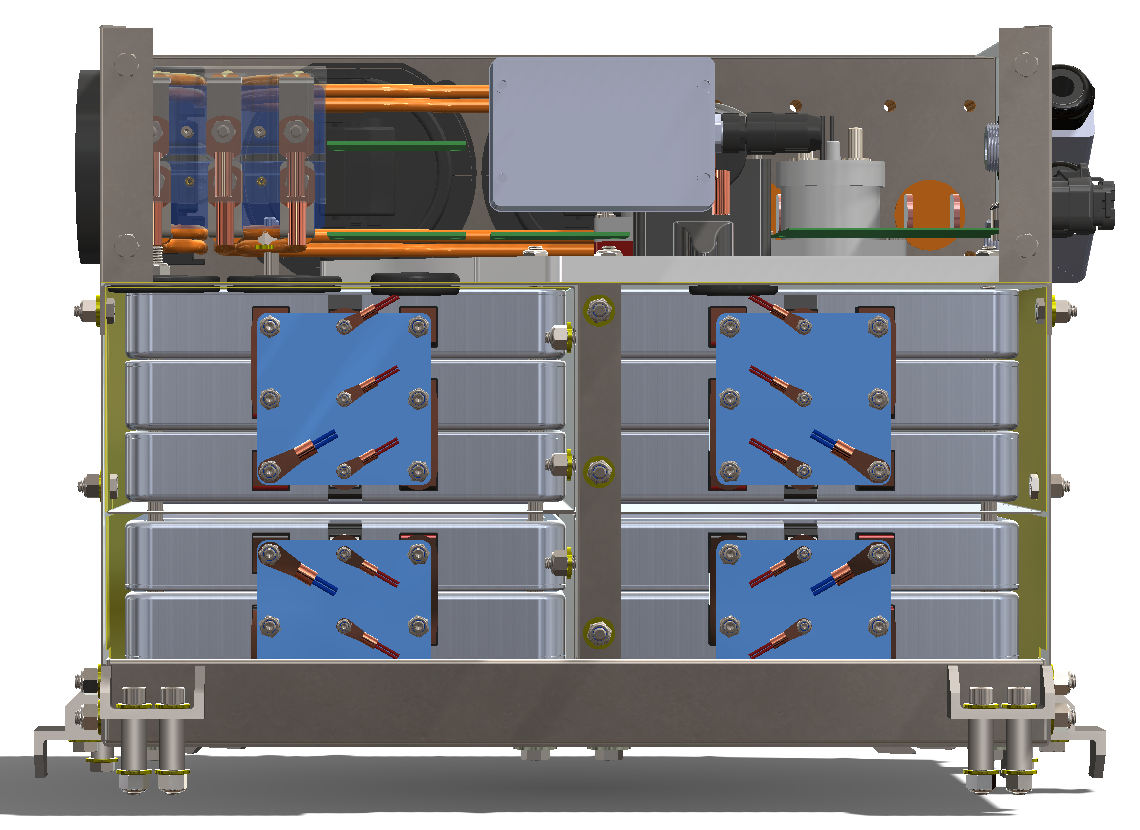
\includegraphics[width = 0.8 \textwidth]{accumulator_frontview}
            \caption{Accumulator, Rear View}
            \label{CADaccumtop}
        \end{figure}

    The AMS monitors 6 groups of cells in series. Each module contains 4 cells, 2 series x 2 parallel, so each AMS monitors 3 modules, or 12 cells (6 series x 2 parallel). There are 4 AMS boards. Each AMS board is coupled to a cell breakout board, which includes 4 thermistors and bolts to the power terminals of three modules, as shown in Figure \ref{CADaccumtop} (blue circuit boards) and described in section \ref{celltopsection}. The purpose of the cell breakout boards is to help manage wiring inside the accumulator. The cell breakout boards will have compression limiting copper pads at the terminal bolts and will be spaced above the bus bars using copper washers. The cell top schematics and PCB CAD are shown in figures \ref{celltopschem} and \ref{celltopboard}.

    The AMS shunts 3 A when the cell gets above the maximum cell voltage. The AMS opens a relay in line with the shutdown circuit if any cell drops below the minimum cell voltage. The AMS opens a relay in line with the shutdown circuit if any cell gets above 60 \degree C (not datasheet value). Please see figure \ref{shutdownschem} for a schematic of the shutdown circuit's relays.

    CAN communication from the board is isolated via a TI ISO1050DUBR (isolated CAN transceiver), with board cutouts to maintain proper clearance and creepage. Only CAN communication is used to have the information from each AMS relayed to the rest of the system, and the boards are otherwise independent of each other. On each cell-top board, there are 7 surface mount Bel C1Q 3 A fuses. (Lowest voltage reference, and top voltage of each of 6 cells.) The relays which allow the AMS to control the shutdown circuit provide isolation between the AMS and the GLV system, as well as the isolated CAN transceivers. Please see Figure \ref{amsschem} on the following page for the schematic of one of the battery management system boards, and the circuitry it has to measure the relative voltage, shunt, and input the data of voltage and temperature to a ATmega16M1 chip (which communicates to the CAN system). Note that the AMS relays are located on neither the cell top board or the AMS boards, but is included in the AIR control board, which controls the power to the AIRs and the precharge/discharge circuitry. The AIR control board is shown in figure \ref{AIRcntrlspacing}, for the pcb spacings. %Its schematic is found in figure \ref{aircntrlschem}

    %SHould I include AIR cntrl??

        \begin{figure}[H]
            \centering
            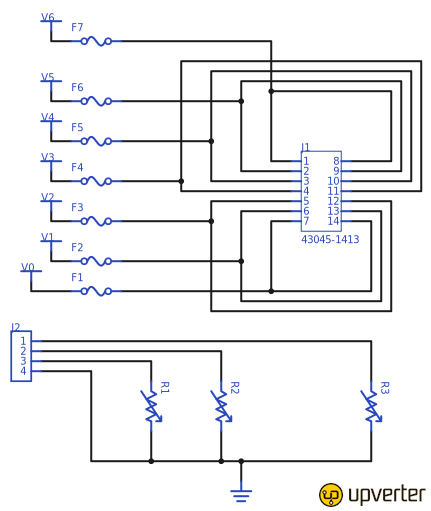
\includegraphics[width = 0.4 \textwidth]{celltopschem}
            \caption{Schematic of the cell-top board}
            \label{celltopschem}
        \end{figure}

        \begin{figure}[H]
            \centering
            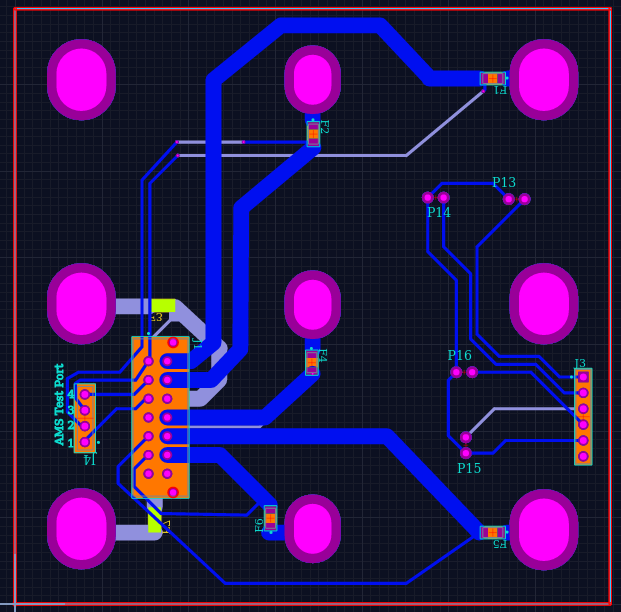
\includegraphics[width = 0.8 \textwidth]{Cell-Top_Boards.png}
            \caption{PCB CAD of the cell-top board}
            \label{celltopboard}
        \end{figure}

                \begin{sidewaysfigure}[p]
                    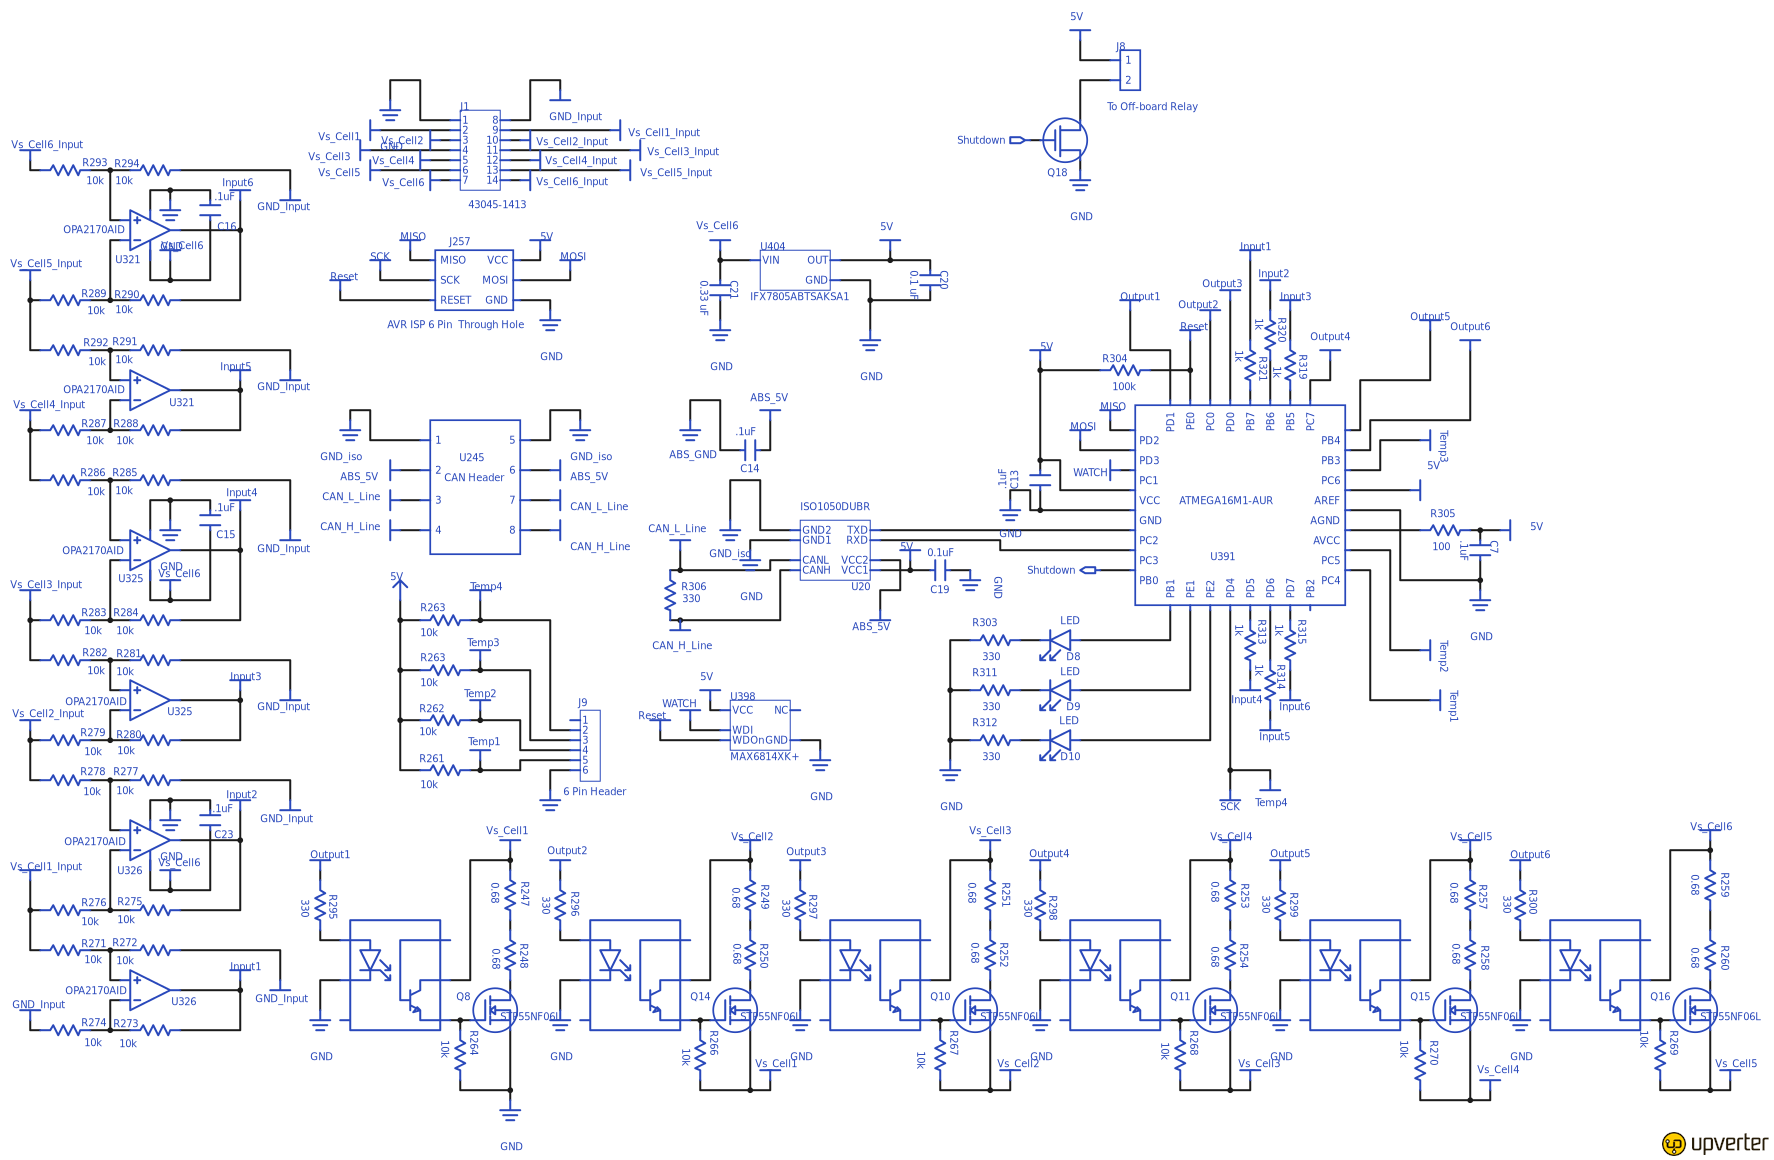
\includegraphics[width=\textheight]{bmsschem}
                    \caption{Accumulator Management System schematic}
                    \label{amsschem}
                \end{sidewaysfigure}

                % \begin{sidewaysfigure}[p]
                %     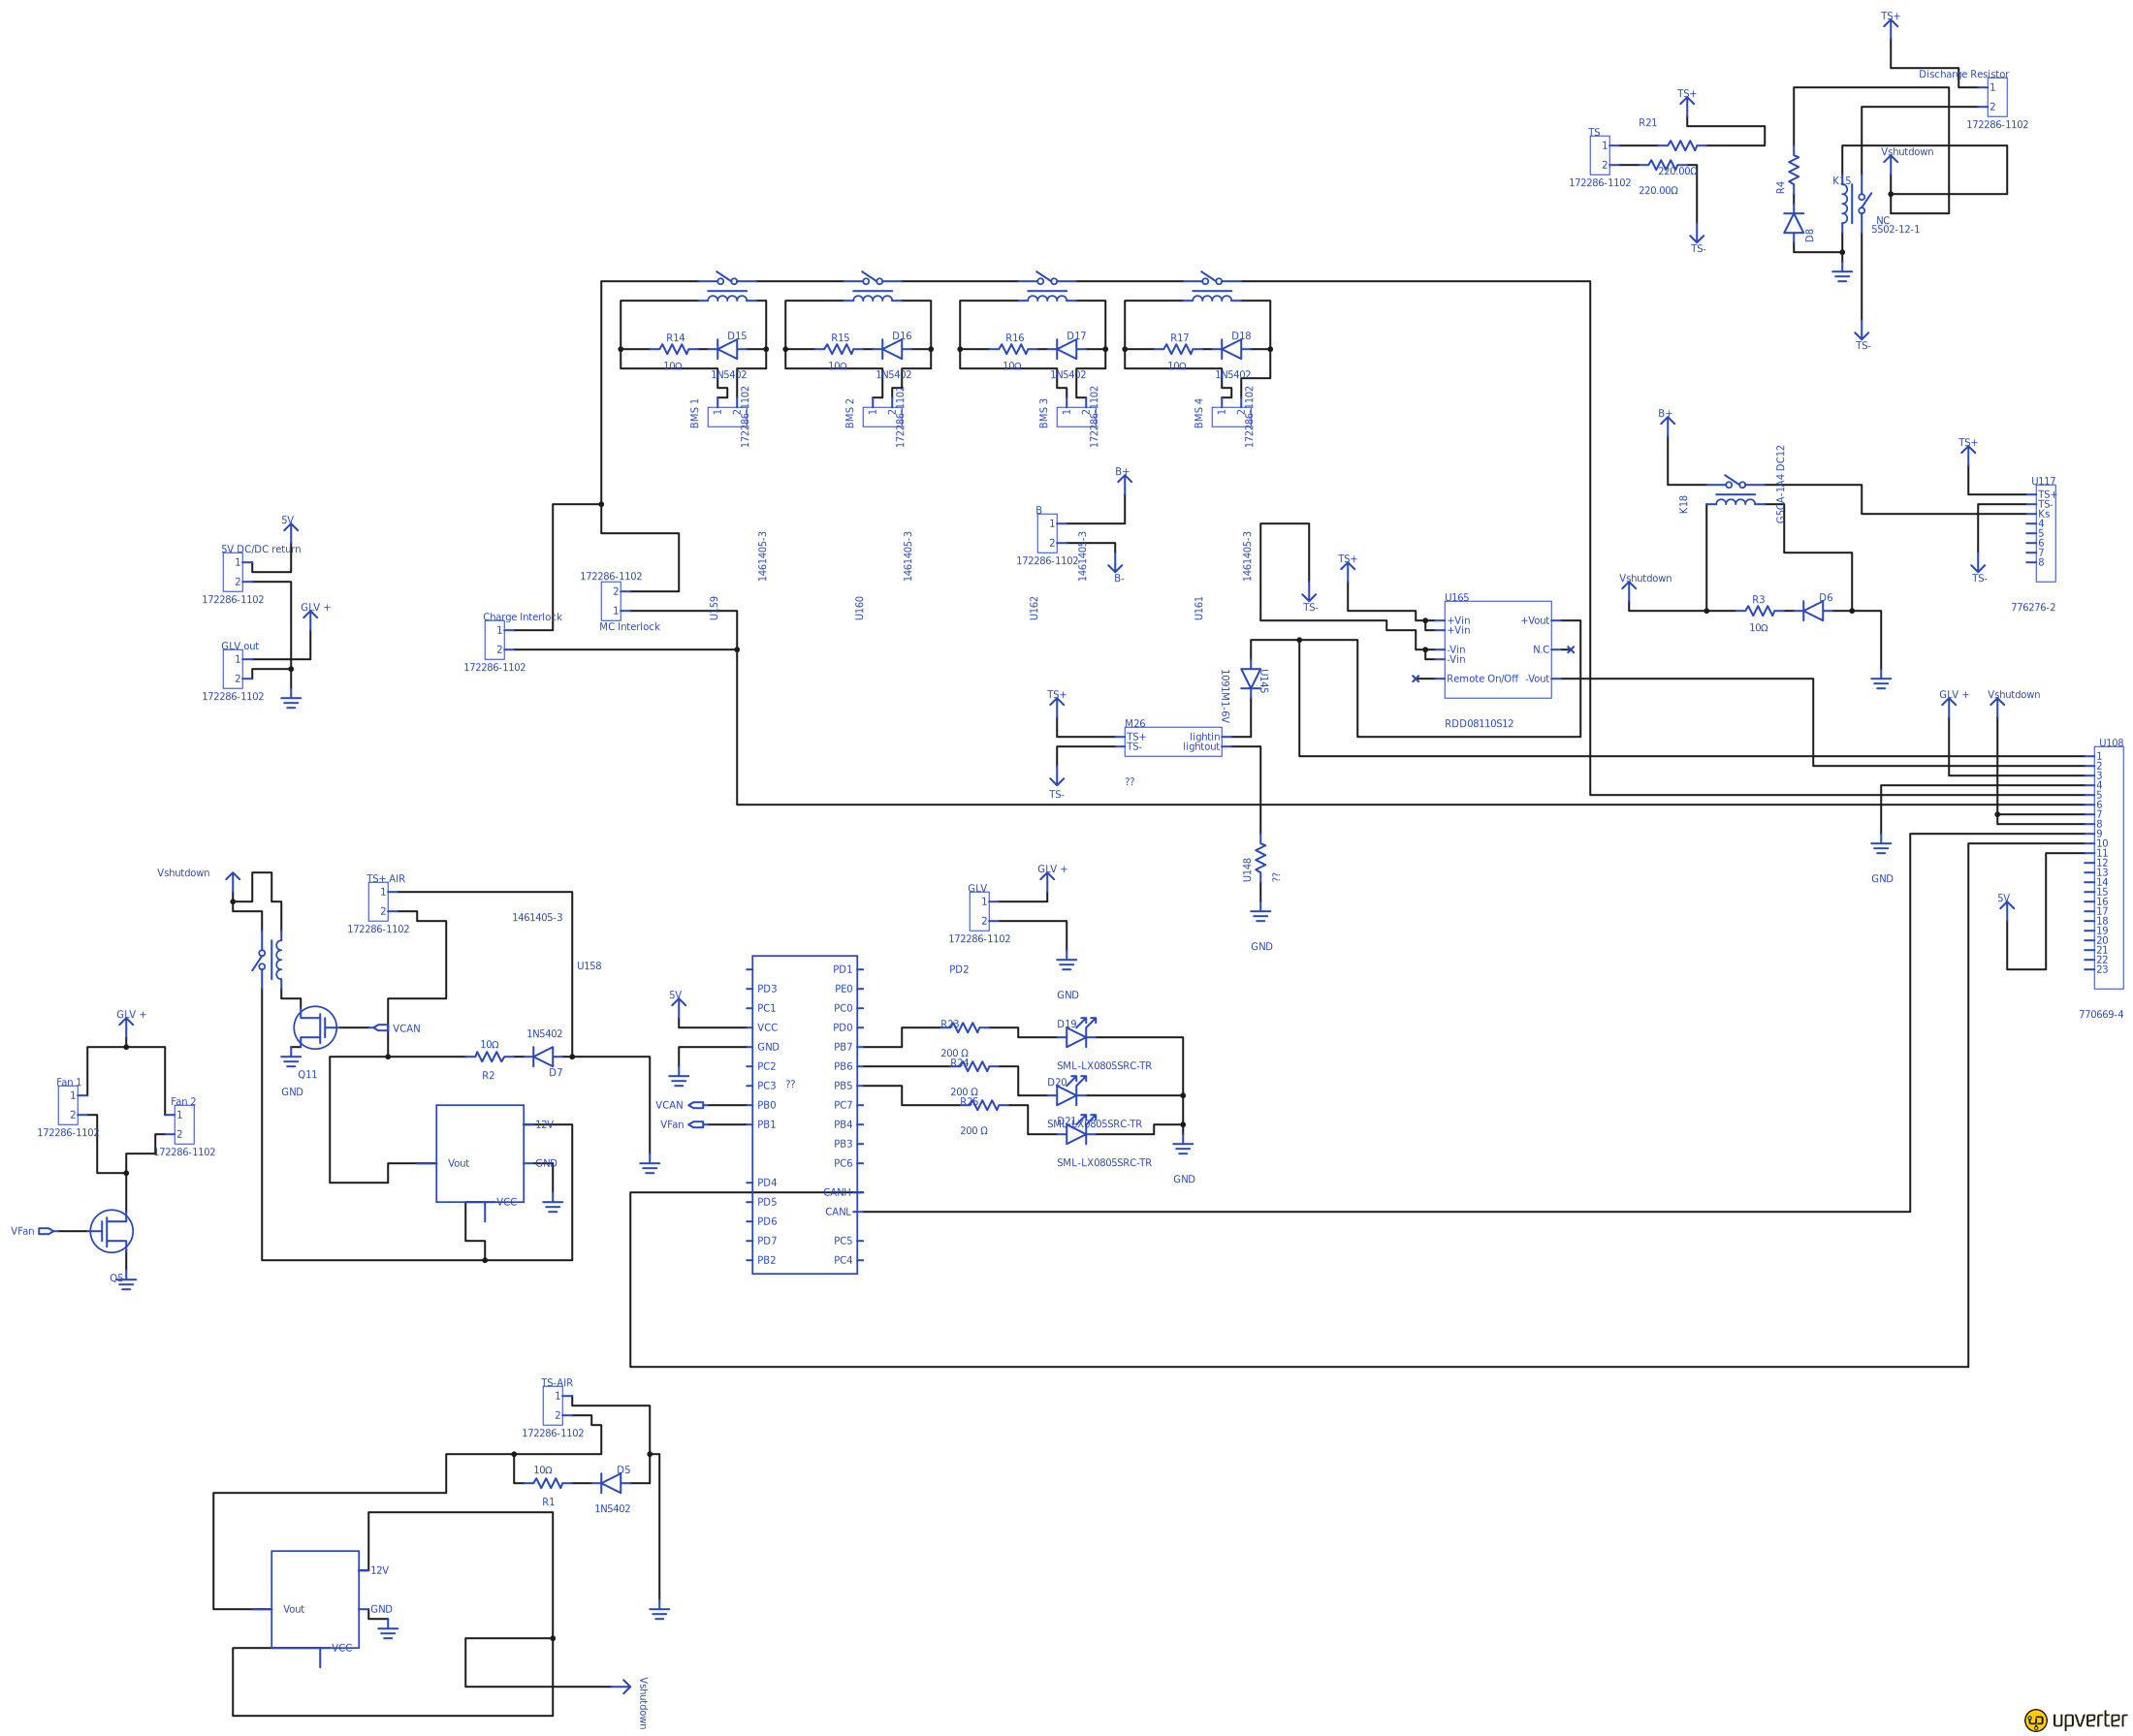
\includegraphics[width=\textheight]{aircntrlschem}
                %     \caption{AIR control board schematic}
                %     \label{aircntrlschem}
                % \end{sidewaysfigure}

\newpage

\subsection{Accumulator Wiring, Cables, Current Calculations}

    \textit{Describe internal wiring with schematics if appropriate. Provide calculations for currents and voltages and show data regarding the cables and connectors used. Discuss maximum expected current, DC and AC, and duration. Compare the maximum values to nominal currents.}

        \begin{figure}[H]
            \centering
            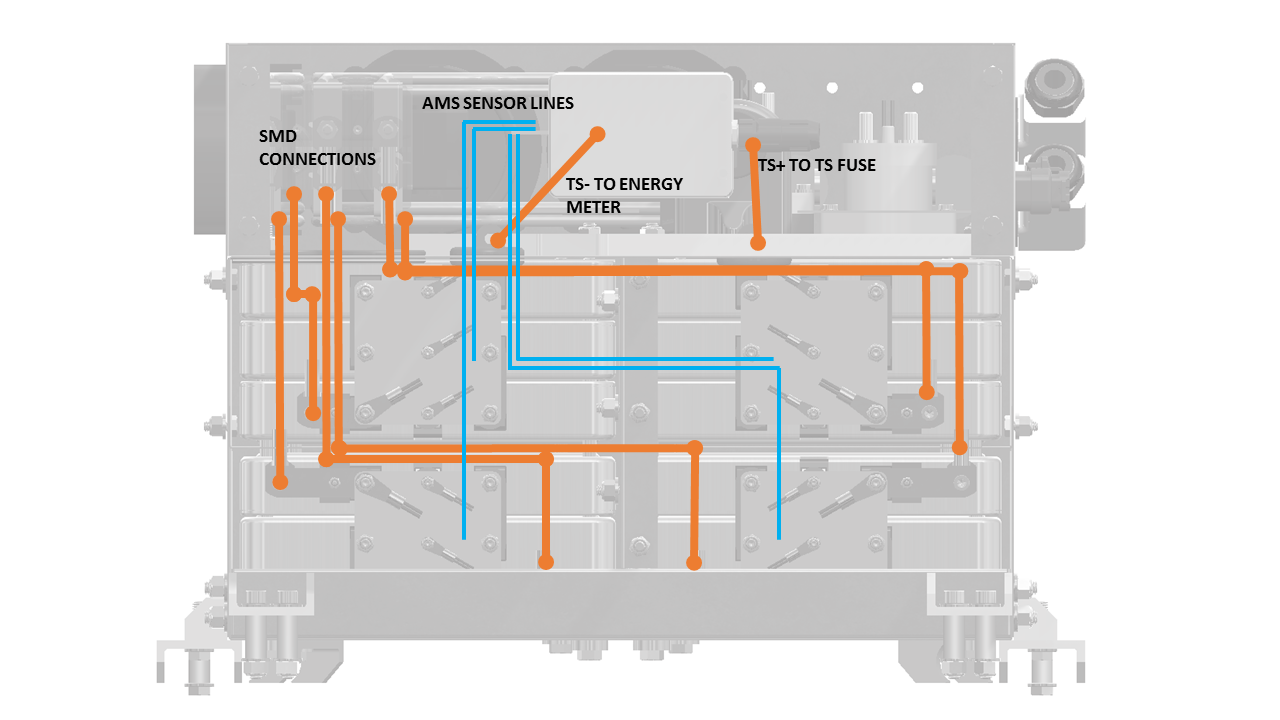
\includegraphics[width = 0.9 \textwidth]{ACCUMULATOR_WIRING_SIDE}
            \caption{Side view of accumulator wiring: All wiring passes through grommeted holes to the top of the pack. Modules within segments are connected using copper bus bars. Cell top boards allow connection of the AMS to individual modules.}
            \label{ACCUMULATOR_WIRING_SIDE}
        \end{figure}

        \begin{figure}[H]
            \centering
            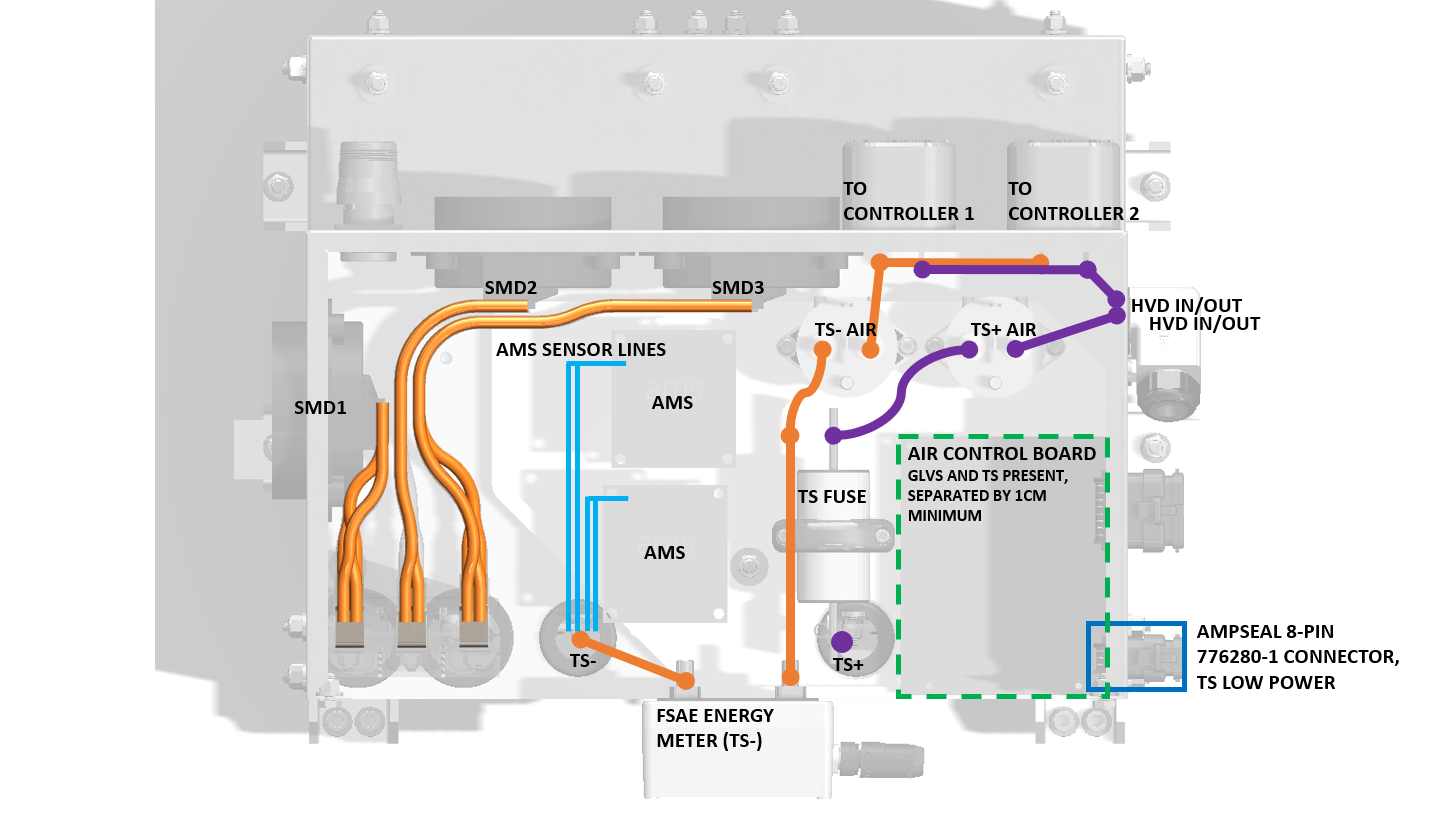
\includegraphics[width = 0.9 \textwidth]{ACCUMULATOR_WIRING_TOP}
            \caption{Top view of accumulator wiring: TS wiring is routed through 3 SMDs in order to segment the accumulator. The pack is fused before the Ts+ AIR then connected to the HVD. The high voltage line is split within the accumulator for the two independent motor controllers. The AMS is located in the center of the pack and monitors cell health during driving and charging. The AIR control Board links the shutdown circuit to the AIRs and is externally connected with AMPSEAL connectors.}
            \label{ACCUMULATOR_WIRING_SIDE}
        \end{figure}

    %10C version - 660 or 650 A is max expected current

\subsection{Accumulator Indicator}

    \textit{If accumulator container is removable, describe the indicator, including indicating voltage range}

        \begin{figure}[H]
            \centering
            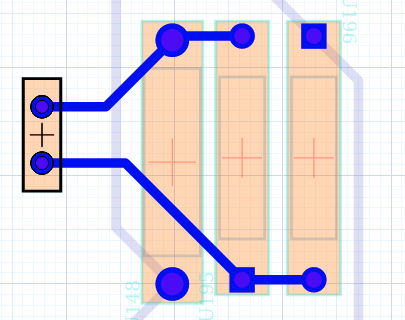
\includegraphics[width = 0.3 \textwidth]{accuindicator}
            \caption{Zoom in on the section of the PCB containing the accumulator indicator (the AIR control board)}
            \label{aindicatorPCB}
        \end{figure}

    The accumulator will be removable and removed each time for the charging process. The accumulator indicator is a small light within the accumulator that can be seen from the outside, and \textcolor{red}{it is powered by a DC-DC converter that is powered by the tractive system}.

\subsection{Charging}

\textit{Describe how the accumulator will be charged. How will the charger be connected? How is the accumulator to be supervised during charging?}

The accumulator will be charged using a Delta Q Technologies QioQ 1000 Series charger (UL listed). This charger has a custom charging process for the accumulator. The charging process is a constant current at 17.0A until the battery voltage reaches 4.15Vpc, and then constant voltage at 4.15Vpc until the current tapers to 2.0A. When charging, the accumulator will be located on a hand cart, with a charging interlock, AMS, emergency stop button, and IMD. These components will make up a small version of the shutdown system in order to protect the accumulator. The charger will connect to the charging connector on the accumulator, and will go through the TS side of the AIRs, connecting to the TS. Therefore, the AMS's, IMD and E-stop will all be able to open the AIRs in the case of an emergency. Also, a person with knowledge of the charging process will stay with the accumulator at all times.

\begin{figure}[H]
    \centering
    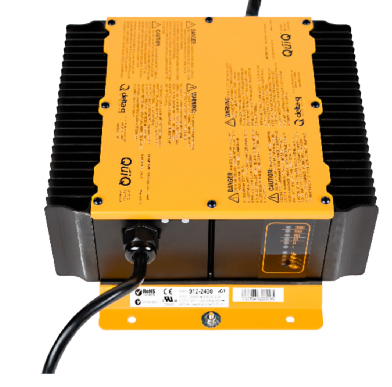
\includegraphics[width = 0.7 \textwidth]{chargepic}
    \caption{Visual of the inteded charger from the Delta Q Technologies QioQ 1000 Series}
    \label{chargepic}
\end{figure}

\begin{table}[H]
\centering
\begin{tabular}{|l|l|}
\hline
Charger Manufacturer and Model & Delta Q Technologies QioQ 1000 Series \\ \hline
Maximum charging power & 70.55 W \\ \hline
% Isolation & Yes/No \\ Yes\hline
% UL Certification & Yes/No \\ Yes\hline
Isolation & Yes \\ \hline
UL Certification & Yes \\ \hline
\begin{tabular}[c]{@{}l@{}}Do you have a waiver from the \\ FH rules committee?\end{tabular} & N/A \\ \hline
Maximum charging voltage & 4.15 V \\ \hline
Maximum charging current & 17.0 A \\ \hline
Interface with accumulator & Connector with interlock \\ \hline
Input voltage & 125VAC or 250VAC \\ \hline
Input current & 13A@125VAC or 10A@250VAC \\ \hline
\end{tabular}
\caption{Charger data}
\label{chargertable}
\end{table}

\subsection{Accumulator Container/Housing}

\textit{Describe the design of the accumulator container. Include the housing material specifications and construction methods. Include data sheets for insulating materials.  Include information documenting compliance with UL94-V0, FAR25 or equivalent.
If the housing is made of conductive material, include information on how the poles of the accumulators are insulated and/or separated from the housing, and describe where and how the container is grounded to the chassis.
Include additional photographs if required to comply with rule EV3.2.
Show how the cells are mounted, use CAD-Renderings, and include calculations showing compliance with FH Rules EV3.4.}

The accumulator is comprised of flanged 403 stainless steel sheetmetal panels, meeting the material and fastener requirements set by Formula SAE Electric rule EV 3.4.6. This rule specifies that the minimum sheet thickness for the floor is 0.049" steel and 0.035" steel for vertical and internal walls. The panels are fastened together using a minimum of three 1/4" SAE Grade 5 at any joint, except at the intersection of internal walls. These intersections, highlighted in gold in Figure \ref{acc_frame}, will be spot welded in at least three places. We will also be conducting a pull-test of test parts to ensure our spot welding settings are correct for full penetration. The Nissan modules are isolated by an additional layer of G10/FR4 Garolite, a fiberglass-cloth with a flame-retardant resin. G10/FR4 meets MIL-I-24768/27 and UL94-V0 for flame retardance (Mcmaster-Carr P/N 8667K55). These barriers do not create electrical insulation, which is performed internal to each module. We have insulation ratings between the Nissan module case and the cell terminals, but this information is under NDA. G10/FR4 panels are highlighted in Figure \ref{acc_iso} in yellow. Please note that not all G10/FR4 panels are not present in our CAD model.

\begin{figure}[H]
    \centering
    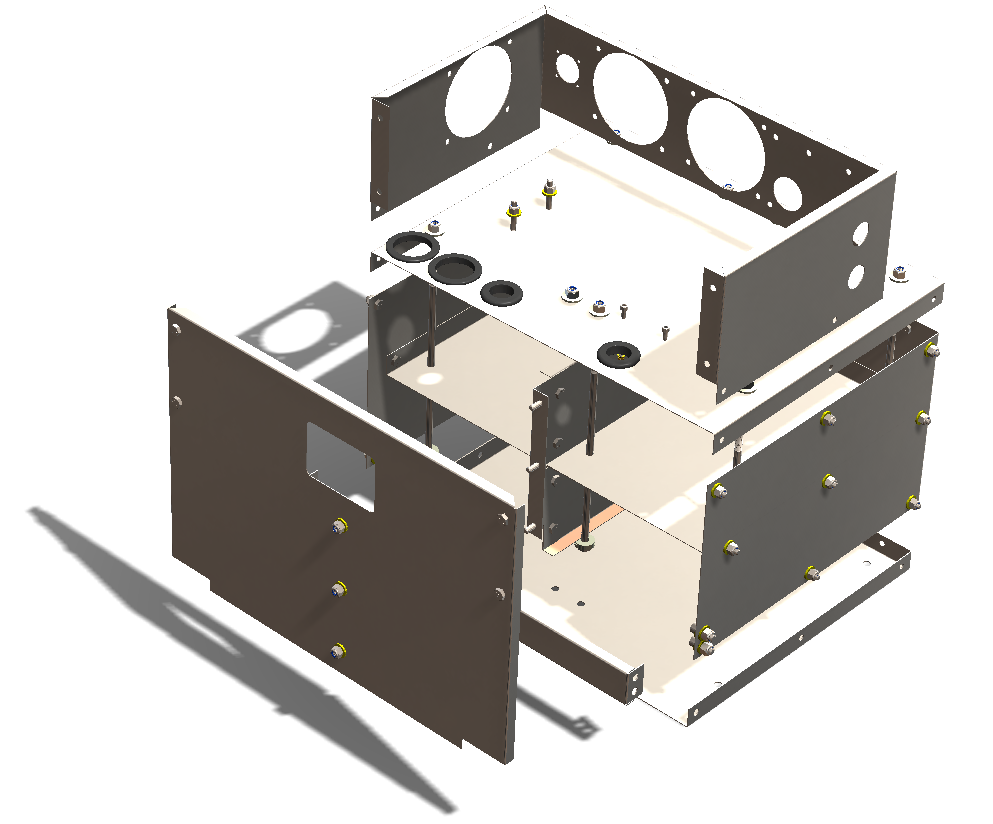
\includegraphics[width = 0.7 \textwidth]{accumulator_frame}
    \caption{Accumulator Frame Exploded View}
    \label{acc_frame}
\end{figure}

\begin{figure}[H]
    \centering
    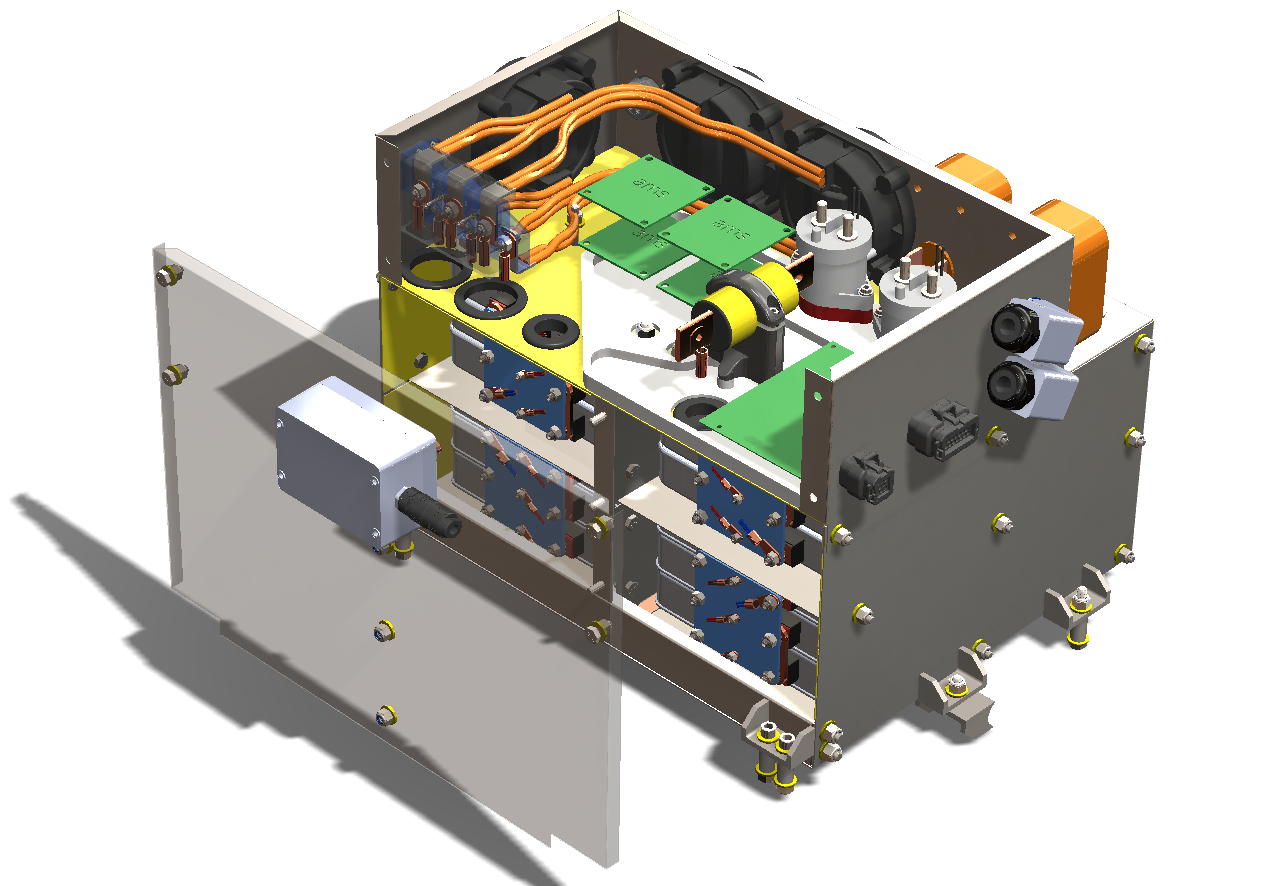
\includegraphics[width = 0.7 \textwidth]{accumulator_isoview}
    \caption{Accumulator, Isometric}
    \label{acc_iso}
\end{figure}

\section{Safety Controls and Indicators}

Person primarily responsible for this section:
    \begin{table}[H]
        \centering
        \label{responsible6}
        \begin{tabular}{lr}
        Name: & Lisa Hachmann \\ \hline
        e-mail: & Lisa.Hachmann@students.olin.edu \\ \hline
        \end{tabular}
    \end{table}

\subsection{Shutdown circuit}

\textit{Include a schematic of the shutdown circuit for your vehicle including all major components in the loop}

%schematic here
Please see figure \ref{shutdownschem} for the shutdown schematic, on the next page.

        \begin{sidewaysfigure}[p]
            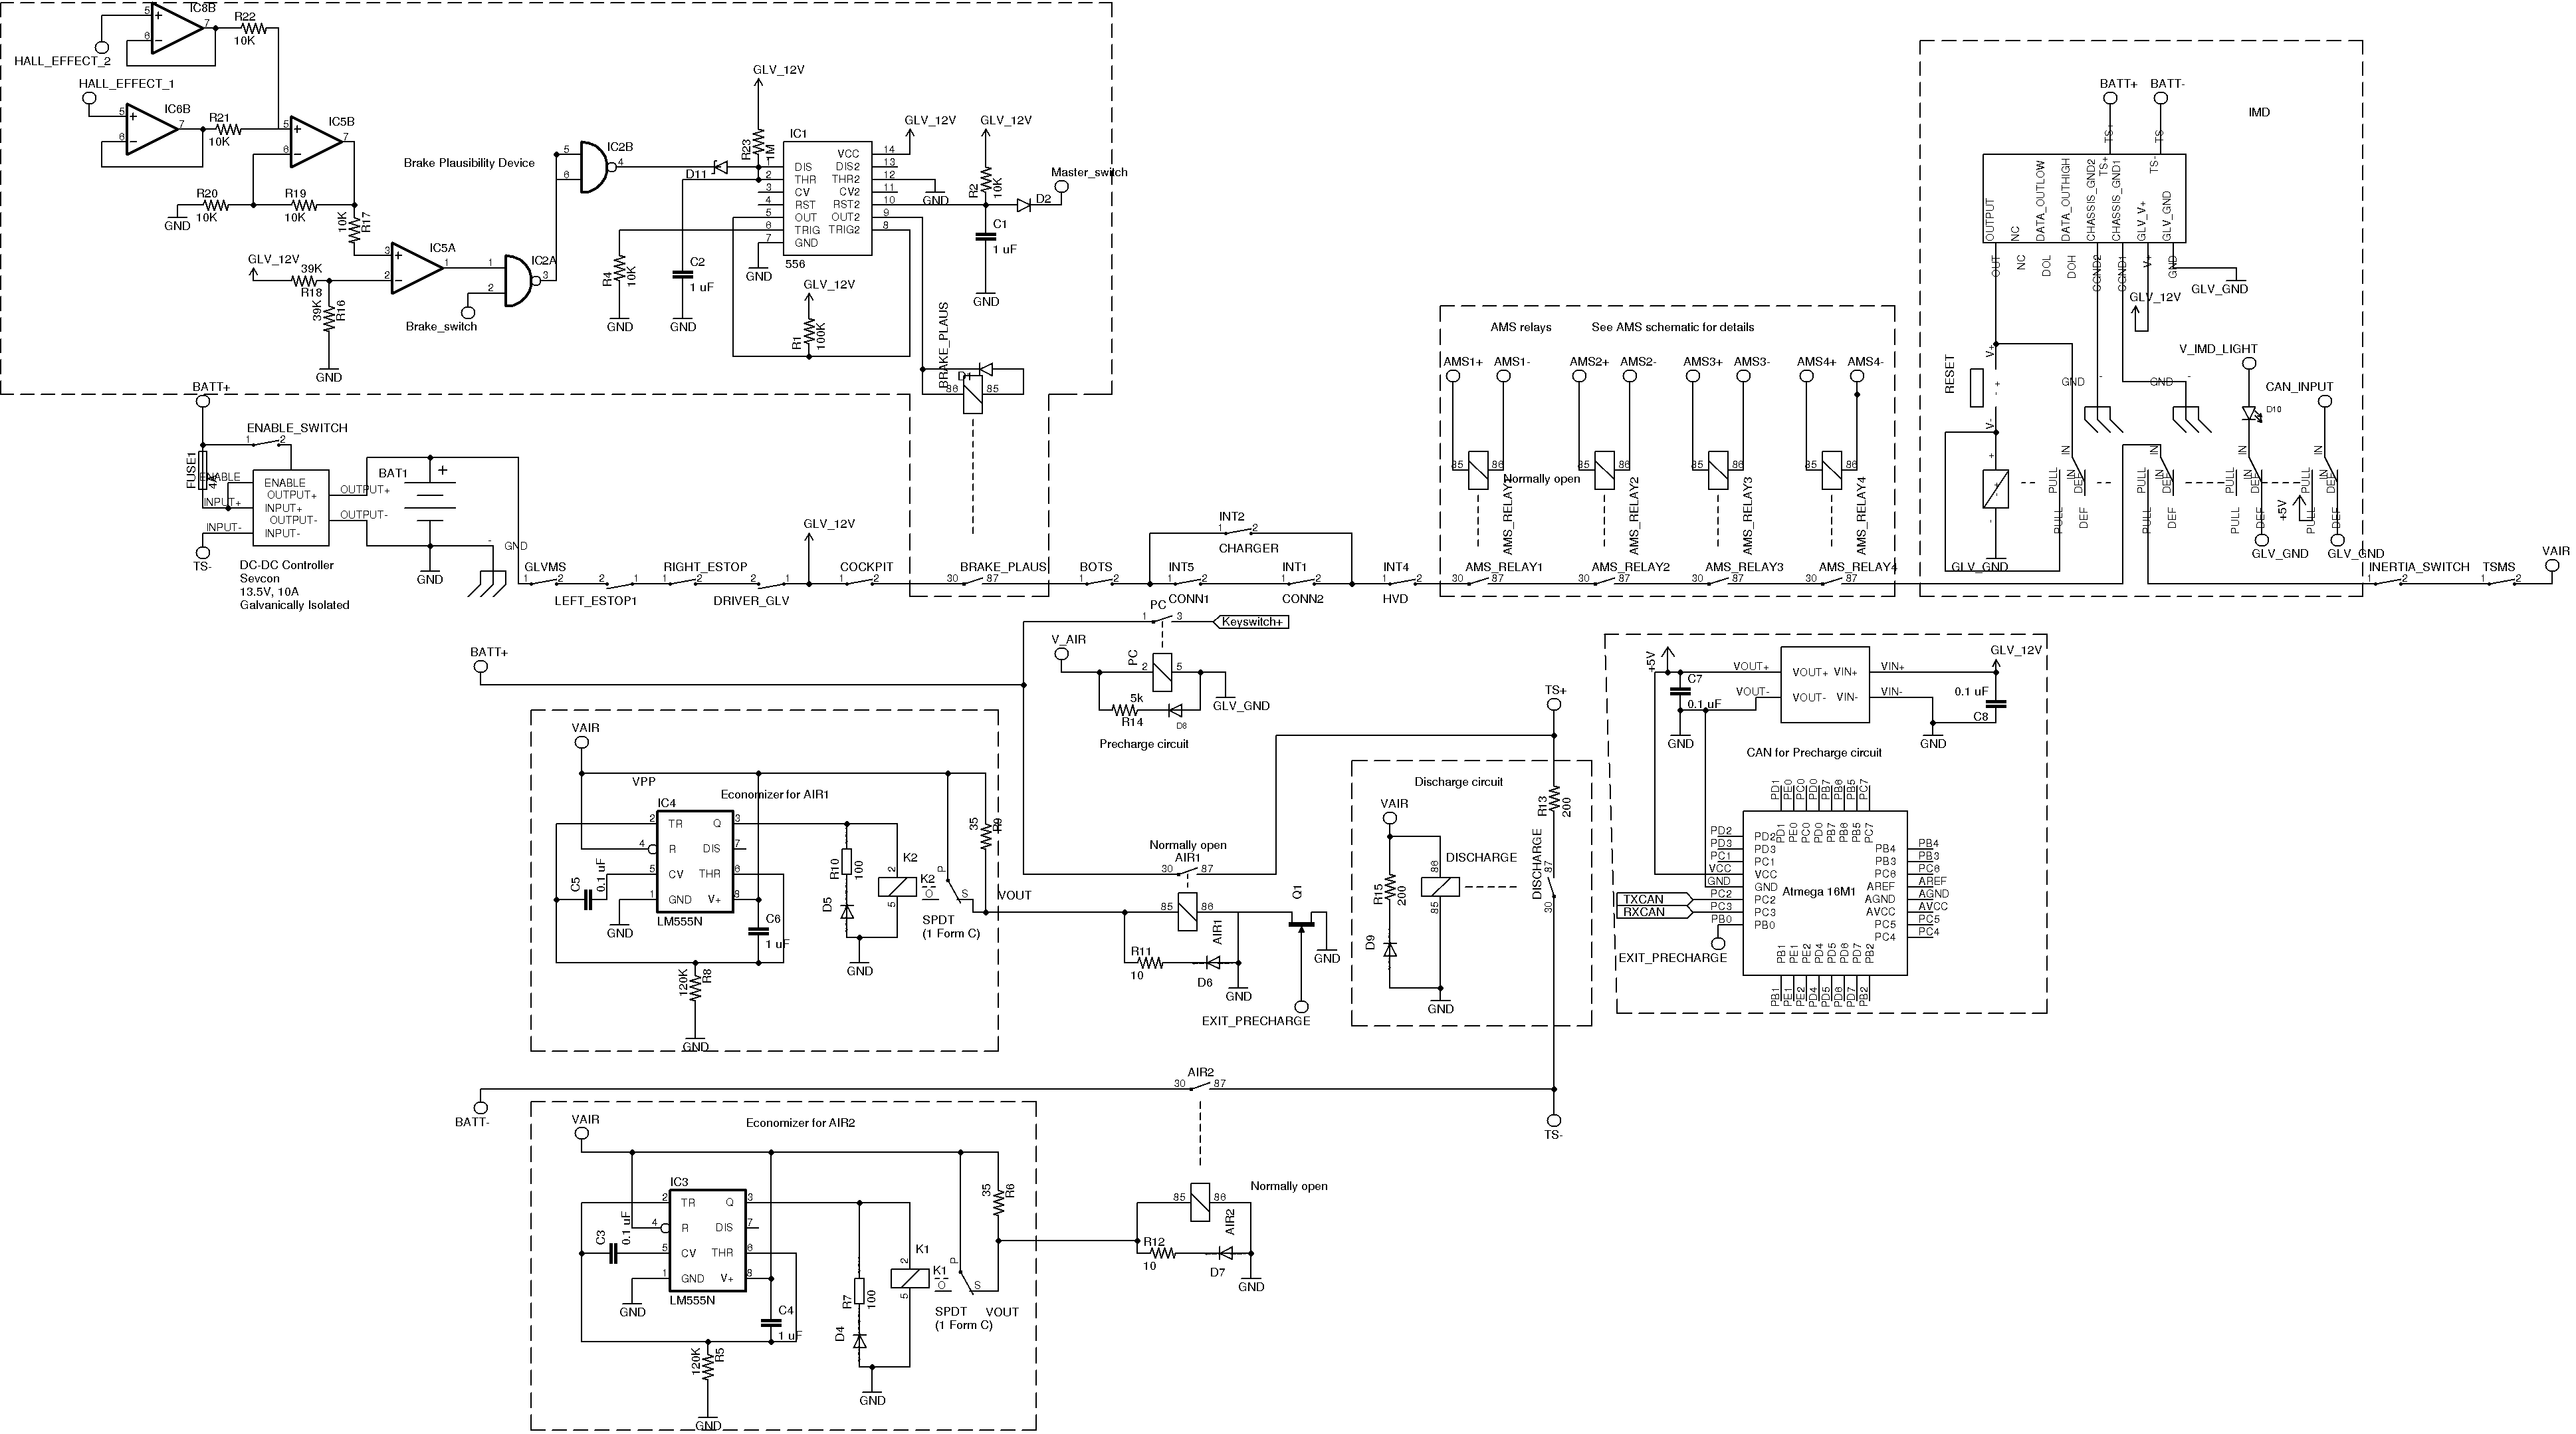
\includegraphics[width=\textheight]{shutdownsystem}
            \caption{Shutdown system schematic}
            \label{shutdownschem}
        \end{sidewaysfigure}


\textit{Describe the method of operation of your shutdown circuit, including the master switches, shut down buttons, brake over-travel switch, etc. Also complete the following table}

The shutdown circuit is a circuit, carrying the power of the AIR all in series. The shutdown circuit utilizes a broad range of sensors for vehicle and driver safety.
The brake over travel switch is a single pole switch that is located behind the brake, and in the event it over-travels, it will open the shutdown circuit.\\

The master switches are single pole switches that must be manually closed in order to close the shutdown system. The keys for the master switches are kept in the active Electrical Safety Officer's possession at all times. When disconnected from the vehicle, the keys are also padlocked to each other, thus disabling closing both switches simultaneously due to the physical separation of the switches and ensuring safety even if the ESO loses possesion of the keys. This ensures that a driver can only operate the vehicle, under the supervision of the ESO.\\

The shutdown buttons are emergency stop buttons that are normally closed and single pole. In the event of the emergency, the three buttons (located in the cockpit, right back and left back of the vehicle) can be pushed and then open the shutdown circuit.\\

The AMS also has relays that carry the power in the shutdown circuit. They are powered by CAN nodes, and are normally open single pole relays. The switch closes the shutdown circuit unless there is a anomaly in the cell voltage or temperature.\\

The IMD constantly checks for ground faults, and has a high output when there is no ground fault. With a high ground fault, if the IMD reset button is pressed, the IMD relay can latch and close the shutdown circuit. \\

Also involved in the shutdown system is a brake over travel switch. This circuitry is built to the FSAE Electric competition rules, and aims to check if there is current flowing from the motor controller while the brake is being pressed (hard). The circuitry cannot include software, so a 555 timer and hall effect sensors are used.\\

The economizer circuitry for the AIRs (in parallel), carry the shutdown circuit and control the AIRs current draw. The economizer is required circuitry by the AIRs used, and lower the continuous current draw through switching.

A switch for GLV power is given to the driver for the ability to see the error messages from CAN. The master switch for the GLV will still need to be closed in order for the driver to be able to gain GLV power.

\begin{table}[H]
\centering
\begin{tabular}{|l|l|}
\hline
Part & \begin{tabular}[c]{@{}l@{}}Function \\ (Momentary, Normally Open or Normally Closed)\end{tabular} \\ \hline
\begin{tabular}[c]{@{}l@{}}Main Switch (for control and \\ tractive-system; CSMS, TSMS)\end{tabular} & Normally Open (x2) \\ \hline
Brake over-travel switch (BOTS) & Normally Closed \\ \hline
Shutdown Buttons (BRB) & Normally Closed (x3) \\ \hline
Insulation Monitoring Device (IMD) & Normally Open \\ \hline
Battery Management System (AMS) & Normally Open (x4) \\ \hline
Interlocks (if used) & Normally Open \\ \hline
GLV switch for the driver & Normally Closed \\ \hline
\end{tabular}
\caption{Switches and devices in the shutdown circuit}
\label{shutdowndevicestable}
\end{table}

\textit{Describe wiring and additional circuitry controlling AIRs. Write a functional description of operation}

The power to the AIRs is all in series until the economizers for each AIR and the AIRs are in parallel. All wiring is 22 AWG and the GLV system is fused to 4A. The shutdown system communicates with the CAN system to ensure simple debugging and software control where permitted.

%table of Shutdown circuit Current Draw
\begin{table}[H]
\centering
\begin{tabular}{|l|l|}
\hline
Total Number of AIRS & 2 \\ \hline
Coil holding current per AIR & \begin{tabular}[c]{@{}l@{}}3.8A until\\ 150 ms passed, \\ then 0.4 A\end{tabular} \\ \hline
\begin{tabular}[c]{@{}l@{}}Current drawn by other components\\ wired in parallel with the AIRs\end{tabular} & 0.5 A \\ \hline
\end{tabular}
\caption{Shutdown circuit current draw}
\label{shutdowncurrenttable}
\end{table}

%CAN x 5 = 250 mA
%555 timers = ~ 50mA
%Hall effect = 12mA*2  = ~25 mA
%Econ relay = 91 mA
%Estimated... 0.5A

\textit{Provide CAD-renderings showing the shutdown circuit parts. Mark the parts in the renderings}

\begin{figure}[H]
    \centering
    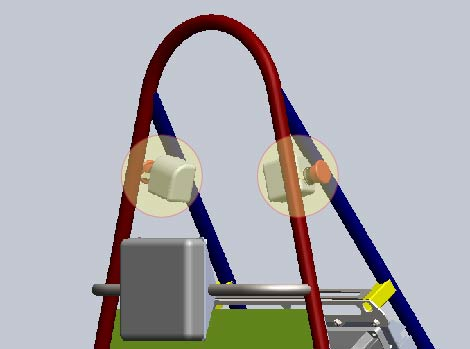
\includegraphics[width = 0.6 \textwidth]{SideMountedShutdownButtons}
    \caption{Side Mounted Shutdown Buttons: Easily visible and accessible for E-Stop rescue scenarios}
    \label{sideshutdown}
\end{figure}

\begin{figure}[H]
    \centering
    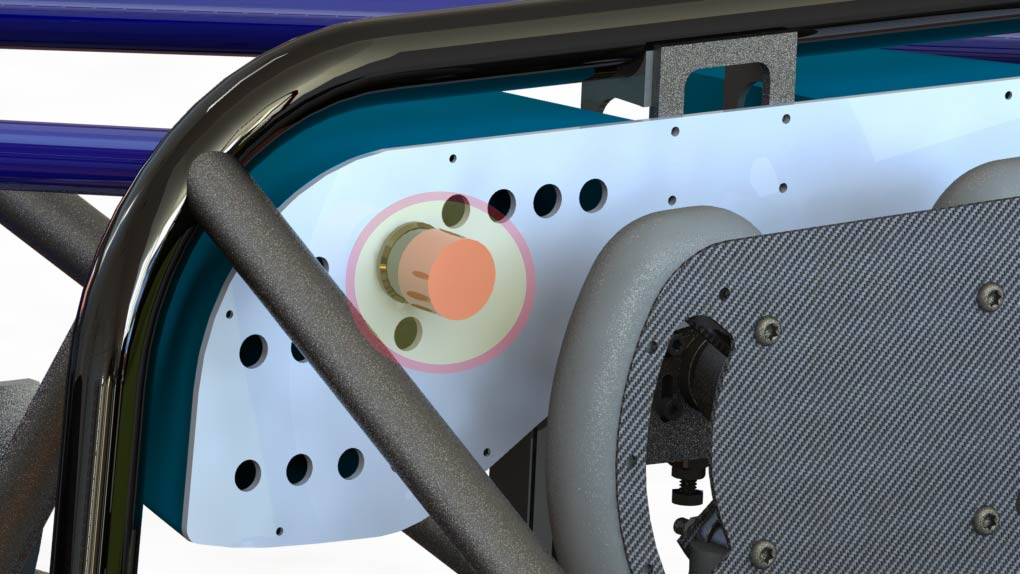
\includegraphics[width = 0.6 \textwidth]{CockpitShutdownButton}
    \caption{Cockpit Shutdown Butto: Large E-Stop button for driver controlled shutdown}
    \label{CockpitShutdownButton}
\end{figure}

\begin{figure}[H]
    \centering
    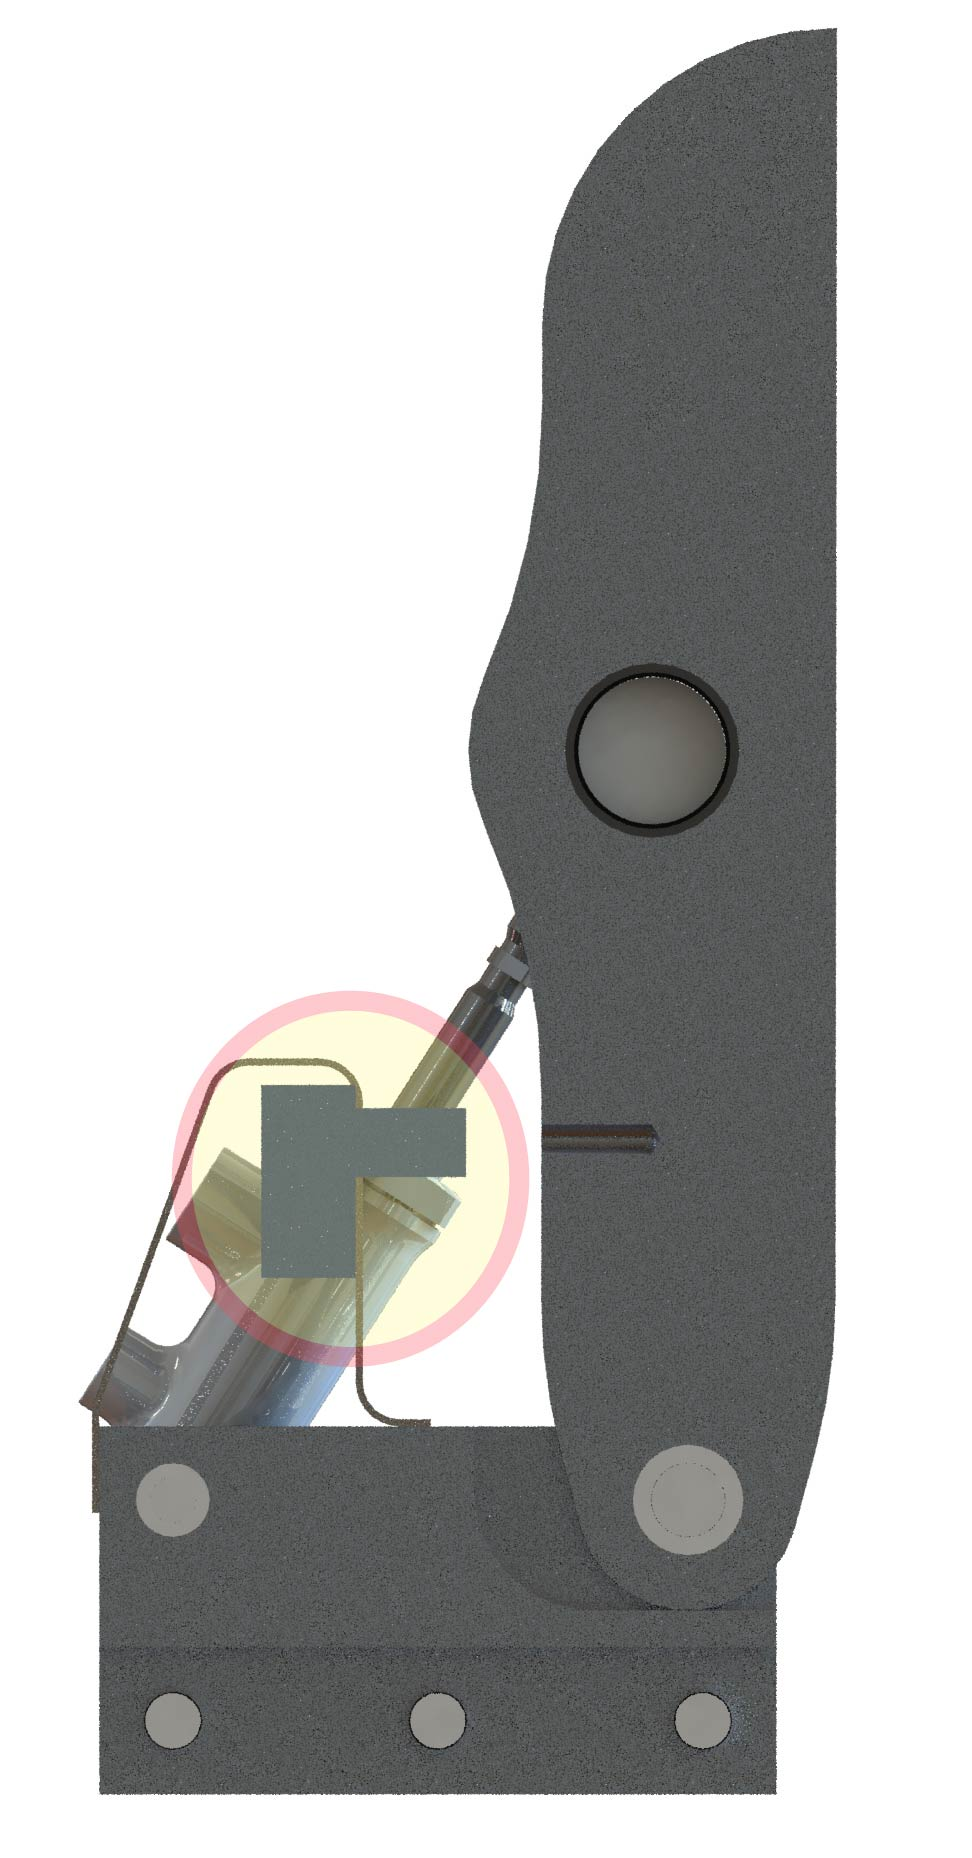
\includegraphics[width = 0.4 \textwidth]{BOTS}
    \caption{Brake Over-travel Switch: The BOTS is mounted to a sheet metal container which is mounted to the pedal assembly. An aluminum nut threaded over the BOTS acts as the positive stop for the pedal, transmitting the pedal load into the sheet metal rather than the switch itself.}
    \label{BOTS}
\end{figure}

\begin{figure}[H]
    \centering
    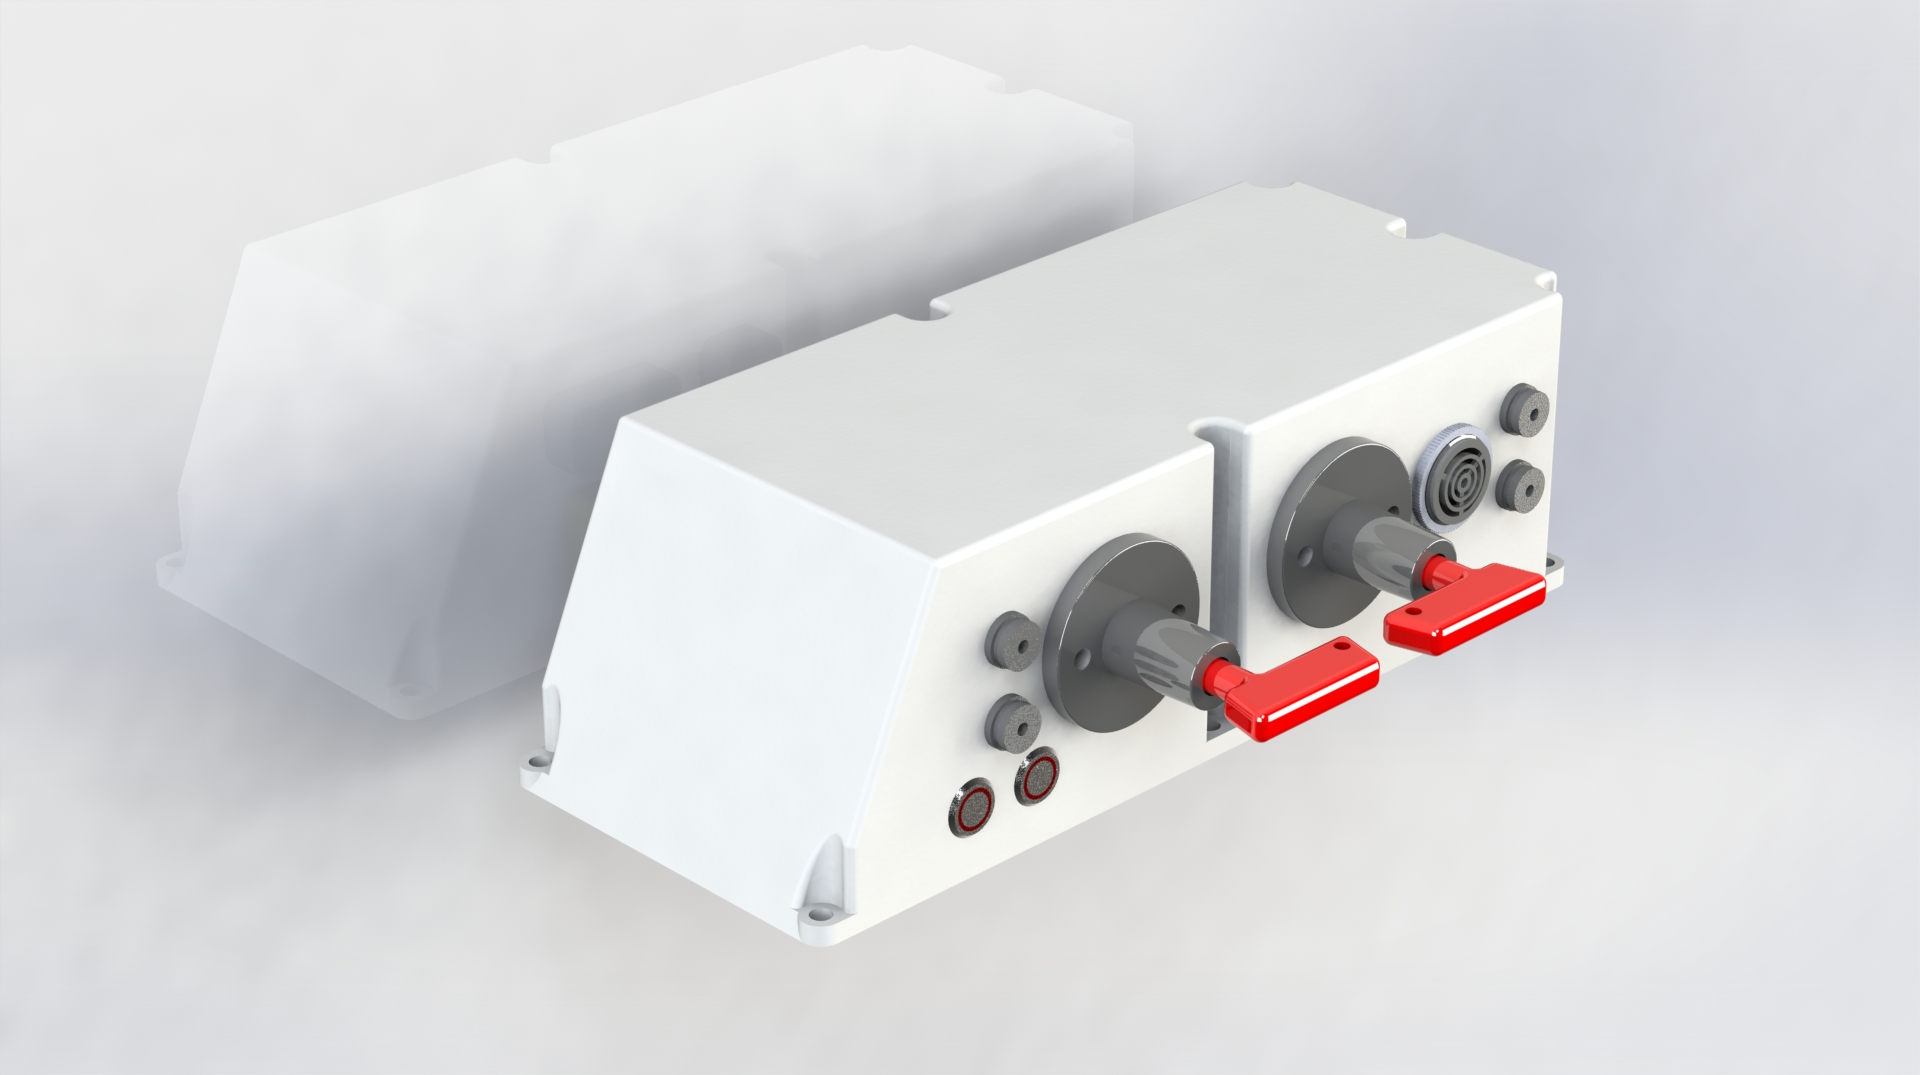
\includegraphics[width = 0.6 \textwidth]{TSMPcontainer1}
    \caption{TSMP Container Front View: The TSMP Container houses the IMD, TSMS, and GLVMS of the shutdown circuit.}
    \label{TSMPcontainer1}
\end{figure}

\begin{figure}[H]
    \centering
    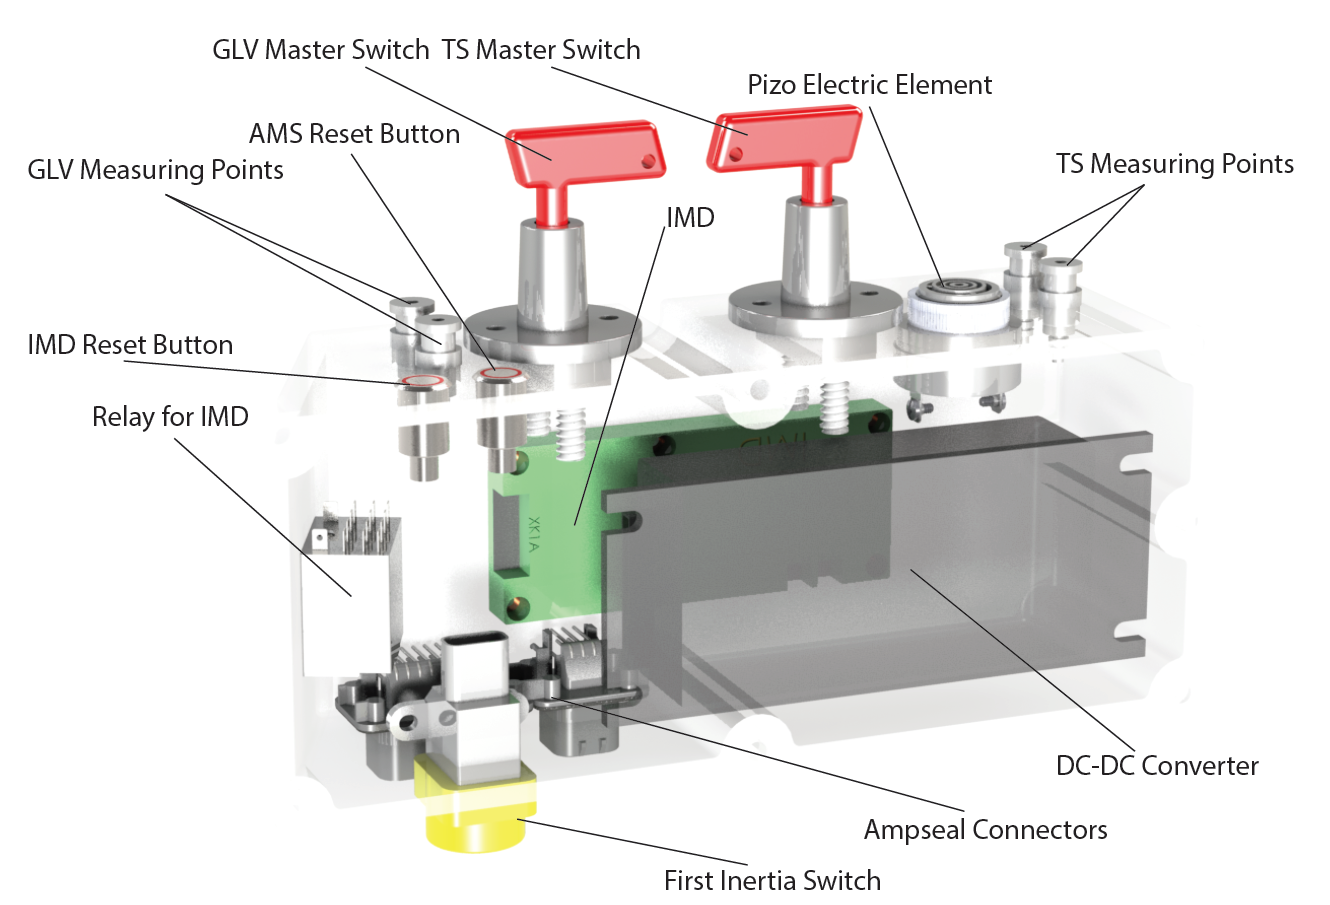
\includegraphics[width = 0.75 \textwidth]{TSMPcontainer2}
    \caption{TSMP Container Top View: The TSMP Container contains TS and GLV systems. Therefore spacing of at least 1 cm is maintained between the two systems at all times. This design is not yet finalized.}
    \label{TSMPcontainer1}
\end{figure}

The physical location of the AMS is pictured and discussed in Figure \ref{ACCUMULATOR_WIRING_SIDE}.

\subsection{IMD}

\textit{Describe the IMD used and use a table for the common operation parameters, like supply voltage, temperature, etc. Describe how the IMD indicator light is wired. Complete the following table. Describe IMD wiring with schematics.}

\begin{figure}[H]
    \centering
    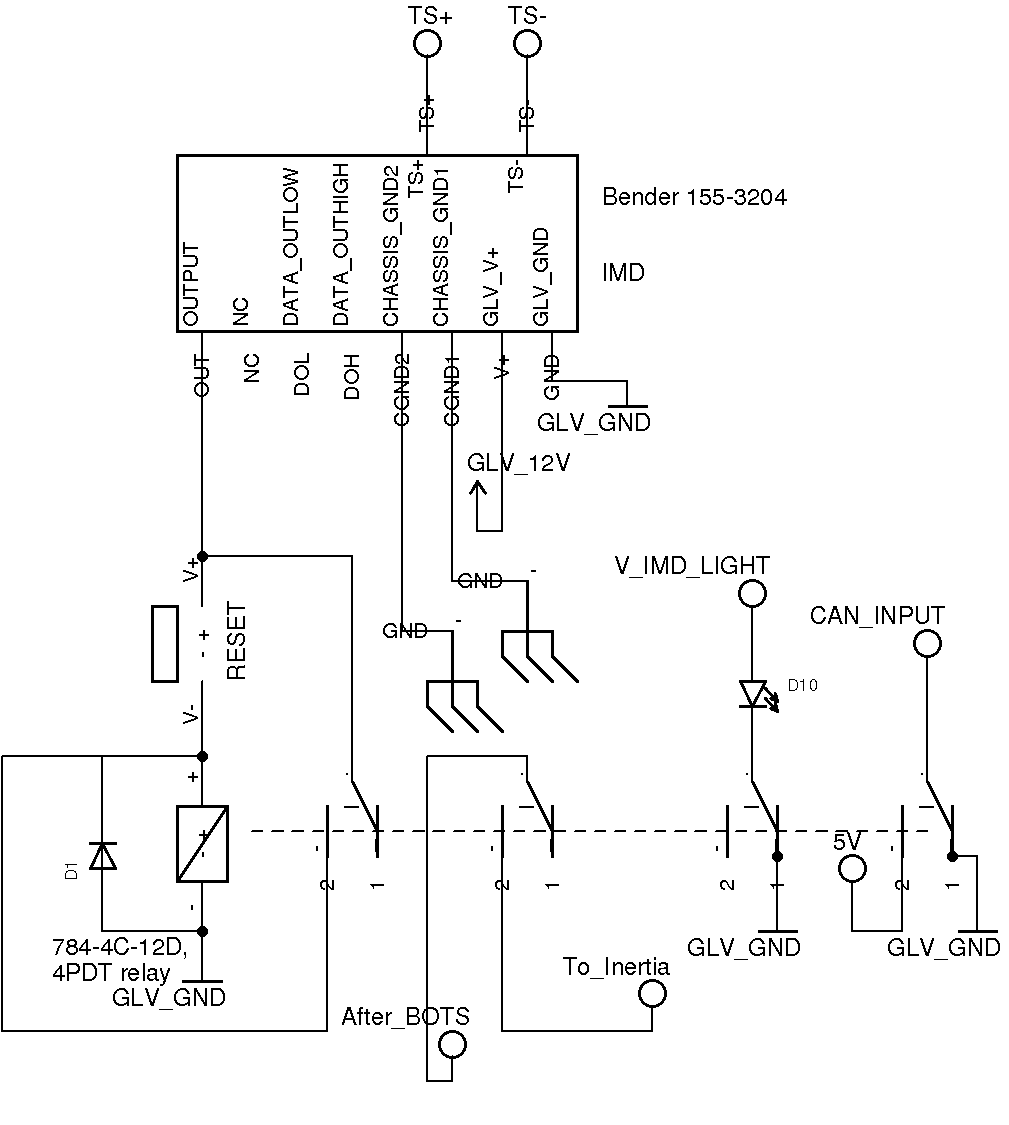
\includegraphics[width = 0.6 \textwidth]{IMDonly}
    \caption{Schematic of the IMD}
    \label{imdschem}
\end{figure}

The IMD will have a high output as long as a there is no ground fault detected. The high output will not power the relay until the reset button is pressed. Pressing the IMD will "latch" it into its state (by using the first switch) until the output goes low from a ground fault. The relay's coil pulls all 4 of the double pole switches to their active states. Therefore, with a latched coil, the switch in the shutdown circuit is closed, the IMD light in the cockpit is not receiving power, and the CAN node input is high.

\begin{table}[H]
\centering
\begin{tabular}{|l|l|}
\hline
MFR/Model & Bender ISOMETER IR155-3204 \\ \hline
Set Response Value & 50 k\ohm \\ \hline
\end{tabular}
\caption{Parameters of the IMD}
\label{IMDtable}
\end{table}

Referred from section \ref{latching} (Reset/Latching for IMD and AMS)

\subsection{Reset / Latching for IMD and AMS} \label{latching}

\textit{Describe the functioning and circuitry of the latching/reset system for a tripped IMD or AMS. Describe wiring, provide schematics.}

If the AMS detects a fault. It opens the shutdown circuit, and latches into that state. When the AMS reset switch, located in the side panel housing, is pressed, the nearby CAN node passes a ”Reset” CAN message to the AMS boards. If the accumulator is within safe electrical and temperature operating limits the AMS closes the shutdown circuit. Figure \ref{amsreset} demonstrates the relevant circuitry of the AMS reset switch and side panel CAN node, which also will be wired to shutdown components.

\begin{figure}[H]
    \centering
    \includegraphics[width = 0.7 \textwidth]{amsreset}
    \caption{Schematic for the AMS reset button and latching}
    \label{amsreset}
\end{figure}

To reset the IMD an operator other than the driver must push the IMD reset button located on the outside of the car on a panel next to the TSMPs, master switches and E-stops. \textcolor{red}{If the output of the IMD is high because there is no ground fault, the reset button will activate the coil and close the shutdown circuit.}

Please see figure \ref{imdschem} for the latching of the IMD circuit. The push button labelled "RESET" is the form of latching for the IMD- pressing the reset button will energize the relay's coil and allow it to self-energize for the remainder of the time that its output is high (true). The IMD reset button must be pressed in order for the shutdown circuit to be closed (assuming the IMD does not find a ground fault).

\subsection{Shutdown System Interlocks}

\textit{(If used) describe the functioning and circuitry of the Shutdown System Interlocks. Describe wiring, provide schematics.}

The shutdown system does employ interlocks on the main battery connectors, and the HVD. The charger's interlock will replace the two main connectors' (to the motor controllers) interlock when the accumulator is charging. All of the interlocks will be fit in their respective high voltage connectors, and be in series with the shutdown circuit, besides the charger interlock being in parallel with the two main connections (referenced as CONN in figure \ref{interlocks}).

\begin{figure}[H]
    \centering
    \includegraphics{interlocks}
    \caption{Schematic of the interlocks as a part of the shutdown circuit}
    \label{interlocks}
\end{figure}

\subsection{Tractive System Energized Light (TSEL)}

\textit{Describe the tractive system energized light components and method of operation. Describe location and wiring, provide schematics. See EV4.10}

\begin{figure}[H]
    \centering
    \includegraphics[width = 0.7 \textwidth]{tsel_fh}
    \caption{Schematic of the TSEL}
    \label{tselschem}
\end{figure}

The TSEL will be located directly under the main roll hoop. It is powered with GLV voltage taken from right before the AIR coils. When 12V is present there, it will close a photomosfet and allow power to pass on the TSAL side.

\subsection{Tractive System Voltage Present light (TSVP)}

\textit{Describe the tractive system voltage present light components and method of operation. Describe location and wiring, provide schematics. See EV4.12}

The TSVPs will be red lights mounted on opposite sides of the roll bar. They are powered when the TS system is over 33VDC, which is 1/3 of the maximum 100V of the TS system. The zener diode circuitry shown in figure \ref{tsvpschem} is used because the breakdown voltage of the zener will power the photo-mosfet when the TS system is over 33VDC, and not before. The lights themselves will be powered off 12V from a DC-DC converter specific to the TS system, which is grounded to the chassis.

\begin{figure}[H]
    \centering
    \includegraphics[width = 0.5 \textwidth]{tsvp_fh}
    \caption{Schematic of the TSVPs}
    \label{tsvpschem}
\end{figure}

\subsection{Ready-To-Drive-Sound (RTDS)}

\textit{Describe your design for the RTDS system. See EV4.11}

The Ready to Drive sound includes a buzzer \href{http://www.mouser.com/ProductDetail/Mallory-Sonalert/SC648ANR/?qs=sGAEpiMZZMsK322k1rNFfUHVVB8ZIcIhitNEhItROC4\%3d}{Mallory Sonalert SC648ANR} (link), a CAN node, and a relay. The buzzer automatically makes a noise when given power, with the loudness proportional to the voltage. The last step in the start-up up sequence will notify the CAN system it is time for the ready to drive sound. Then the corresponding node on the buzzer will close a relay between TS+, after a 2.6 k\ohm resistor (5 Watts), and the buzzer for two seconds, at 95 dB at 2ft. The resistor limits the voltage over the buzzer to 48V and the current to 20 mA.

\begin{figure}[H]
    \centering
    \includegraphics{R2Dsoundbuzzerschem}
    \caption{Schematic for the Ready to Drive Sound}
    \label{r2dschem}
\end{figure}

\section{GLV system}
Person primarily responsible for this section:

    \begin{table}[H]
        \centering
        \label{responsible7}
        \begin{tabular}{lr}
        Name: & Byron Wasti \\ \hline
        e-mail: & Byron.wasti@students.olin.edu \\ \hline
        \end{tabular}
    \end{table}

\subsection{GLV System Data}

\textit{Provide a brief description of the GLV system and complete the following table}\\

\textnormal{The GLV system consists of nine separate CAN nodes and all peripheral sensors. There will be a 12V line, 5V line, CAN High and CAN Low going along the car in order to power different components and to allow communications.}

\begin{table}[H]
\centering
\begin{tabular}{|l|l|}
\hline
GLV System Voltage & 12V \\ \hline
GLV Main Fuse Rating & 4A \\ \hline
Is a Li-Ion GLV battery used? & No \\ \hline
If Yes, is a firewall provided per T4.5.1? & N/A \\ \hline
Is a DC-DC converter used from TSV? & Yes \\ \hline
Is the GLV system grounded to the chassis? & Yes \\ \hline
Does the design comply with EV1.2.7? & Yes \\ \hline
\end{tabular}
\caption{GLV System Data}
\label{glvtable}
\end{table}

\section{Appendices}

Include only highly-relevant data. A link to a web document in the ESF text is often more convenient for the reviewer.

\textcolor{red}{The specification section of the accumulator data sheet, and sections used for determining accumulator capacity (FH Rules Appendix A) should be included here.}

% Maybe consider adding some sort of intro or something here

%The specification section of the accumulator data sheet, and sections used for determining accumulator capacity (FH Rules Appendix A) should be included here.
%secret blue cursor
%Who are you
%I love you blue cursor  Plus I can move you around wherever I want! Haha! You're under my control no w  woooo yeah look at me moving your cursor around yeah blue cursor you go where I tell you to go suck on that

%\includepdf[pages=-]{GMNissanInfo.pdf}

\includepdf[pages=-]{LiMn2O4_MSDS.pdf}

\includepdf[pages=-]{LiMn2O4_MSDS.pdf}

%MSDS Sheets must be included for the accumulator cells

\begin{figure}[H]
    \centering
    \includegraphics[width = 0.7 \textwidth]{appendixa}
    \caption{Selection of Appendix A used to determine accumulator capacity}
    \label{appendixa}
\end{figure}

\href{http://delta-q.com/product/quiq-1000-industrial-battery-charger/}{Charger (QuiQ 1000 Series, Delta Q Technologies, specifications }

\end{document}
